
%%%%%%%%%%%%%%%%%%%%%%%%%%%%%%%%%%%%%%%%%%%%%%%%%%%%%%%%
%
% Copyright (c) 2003-2011 by University of Queensland
% Earth Systems Science Computational Center (ESSCC)
% http://www.uq.edu.au/esscc
%
% Primary Business: Queensland, Australia
% Licensed under the Open Software License version 3.0
% http://www.opensource.org/licenses/osl-3.0.php
%
%%%%%%%%%%%%%%%%%%%%%%%%%%%%%%%%%%%%%%%%%%%%%%%%%%%%%%%%

\documentclass{esysdoc}
%%% Table of contents to list down to subsections and no further
\setcounter{tocdepth}{3}
%%% Number down to subsubsections only
\setcounter{secnumdepth}{3}
% grab the handy definitions and \usepackage statements etc

%%%%%%%%%%%%%%%%%%%%%%%%%%%%%%%%%%%%%%%%%%%%%%%%%%%%%%%%%%%%%%%%%%%%%%%%%%%%%%
% Copyright (c) 2003-2017 by The University of Queensland
% http://www.uq.edu.au
%
% Primary Business: Queensland, Australia
% Licensed under the Apache License, version 2.0
% http://www.apache.org/licenses/LICENSE-2.0
%
% Development until 2012 by Earth Systems Science Computational Center (ESSCC)
% Development 2012-2013 by School of Earth Sciences
% Development from 2014 by Centre for Geoscience Computing (GeoComp)
%
%%%%%%%%%%%%%%%%%%%%%%%%%%%%%%%%%%%%%%%%%%%%%%%%%%%%%%%%%%%%%%%%%%%%%%%%%%%%%%

\usepackage{subfigure}
\usepackage{epsfig}

\usepackage{graphicx,color}
% \usepackage[pdftex]{graphicx,color}
\usepackage{makeidx}  % handle the index properly
\usepackage{xspace}   % handle spaces after commands more nicely
% use the ams math stuff, as it makes the maths easier to code, and
% nicer output than the standard LaTeX stuff
\usepackage{amsmath,amsfonts,amssymb} % this is handy for mathematicians and physici % see http://www.ams.org/tex/amslatex.html
\usepackage{alltt}   % handy verbatim stuff
\usepackage{textcomp}
\usepackage{setspace}
%\usepackage{movie15}
% Special Formatting Packages
% Colour Package
\usepackage[usenames,dvipsnames]{xcolor}
% Assignm Colour Names and import hyperlinks.
\usepackage{float}
%\usepackage[unicode,colorlinks=true,linkcolor=NavyBlue,citecolor=OliveGreen,urlcolor=Plum]{hyperref}

% Fancy Verb


\usepackage[numbers]{natbib}
\usepackage{chapterbib}
\renewcommand{\bibname}{References}

%\doublespacing

%% Python listing setup
% from http://blog.miliauskas.lt/2008/09/python-syntax-highlighting-in-latex.html

\usepackage{color}
\usepackage[procnames]{listings}
\usepackage{textcomp}
\usepackage{setspace}
\usepackage{palatino}
\renewcommand{\lstlistlistingname}{Code Listings}
\renewcommand{\lstlistingname}{Code Listing}
\definecolor{gray}{gray}{0.5}
\definecolor{green}{rgb}{0,0.5,0}
\definecolor{lightgreen}{rgb}{0,0.7,0}
\definecolor{purple}{rgb}{0.5,0,0.5}
\definecolor{darkred}{rgb}{0.5,0,0}
\definecolor{orange}{rgb}{1.0,0.4,0.1}
\lstnewenvironment{python}[1][]{
\lstset{
language=python,
basicstyle=\ttfamily\small\setstretch{1},
stringstyle=\color{green},
showstringspaces=false,
alsoletter={1234567890},
otherkeywords={\ , \}, \{},
keywordstyle=\color{blue},
emph={access,and,as,break,class,continue,def,del,elif,else,%
except,exec,finally,for,from,global,if,import,in,is,%
lambda,not,or,pass,print,raise,return,try,while,assert},
emphstyle=\color{orange}\bfseries,
emph={[2]self},
emphstyle=[2]\color{gray},
emph={[4]ArithmeticError,AssertionError,AttributeError,BaseException,%
DeprecationWarning,EOFError,Ellipsis,EnvironmentError,Exception,%
False,FloatingPointError,FutureWarning,GeneratorExit,IOError,%
ImportError,ImportWarning,IndentationError,IndexError,KeyError,%
KeyboardInterrupt,LookupError,MemoryError,NameError,None,%
NotImplemented,NotImplementedError,OSError,OverflowError,%
PendingDeprecationWarning,ReferenceError,RuntimeError,RuntimeWarning,%
StandardError,StopIteration,SyntaxError,SyntaxWarning,SystemError,%
SystemExit,TabError,True,TypeError,UnboundLocalError,UnicodeDecodeError,%
UnicodeEncodeError,UnicodeError,UnicodeTranslateError,UnicodeWarning,%
UserWarning,ValueError,Warning,ZeroDivisionError,abs,all,any,apply,%
basestring,bool,buffer,callable,chr,classmethod,cmp,coerce,compile,%
complex,copyright,credits,delattr,dict,dir,divmod,enumerate,eval,%
execfile,exit,file,filter,float,frozenset,getattr,globals,hasattr,%
hash,help,hex,id,input,int,intern,isinstance,issubclass,iter,len,%
license,list,locals,long,map,max,min,object,oct,open,ord,pow,property,%
quit,range,raw_input,reduce,reload,repr,reversed,round,set,setattr,%
slice,sorted,staticmethod,str,sum,super,tuple,type,unichr,unicode,%
vars,xrange,zip},
emphstyle=[4]\color{purple}\bfseries,
upquote=true,
morecomment=[s][\color{lightgreen}]{"""}{"""},
commentstyle=\color{red}\slshape,
literate={>>>}{\textbf{\textcolor{darkred}{>{>}>}}}3%
         {...}{{\textcolor{gray}{...}}}3,
procnamekeys={def,class},
procnamestyle=\color{blue}\textbf,
%framexleftmargin=1mm, framextopmargin=1mm, frame=box,
%rulesepcolor=\color{gray},#1
}}{}



%%%%%%%%%%%%%%%%%%%%%%%%%%%%%%%%%%%%%%%%%%%%%%%%%%%%%%%%%%%%%%%%%%%%%%%%%%%%%%
% Copyright (c) 2003-2015 by University of Queensland
% http://www.uq.edu.au
%
% Primary Business: Queensland, Australia
% Licensed under the Open Software License version 3.0
% http://www.opensource.org/licenses/osl-3.0.php
%
% Development until 2012 by Earth Systems Science Computational Center (ESSCC)
% Development 2012-2013 by School of Earth Sciences
% Development from 2014 by Centre for Geoscience Computing (GeoComp)
%
%%%%%%%%%%%%%%%%%%%%%%%%%%%%%%%%%%%%%%%%%%%%%%%%%%%%%%%%%%%%%%%%%%%%%%%%%%%%%%

\usepackage{listing}
% defines the colour for the background of code examples
\definecolor{LightGrey}{gray}{0.9}

%Some colour definitions added to keep pdflatex happy
%I make no claim that these values are particularly good
\definecolor{Purple}{rgb}{0.7, 0, 0.6}
\definecolor{Tan}{rgb}{0.5,0.5,0.5}
\definecolor{BrickRed}{rgb}{0.7, 0.2, 0.2}
\definecolor{Black}{rgb}{0, 0, 0}

% All the \color{x} used to be \color[named]{x}
%end color defs

\lstdefinestyle{myC++}{%
language=C++,
showstringspaces=false,
basicstyle=\small\ttfamily,
commentstyle=\color{BrickRed}\ttfamily,
keywordstyle=\color{Purple}\ttfamily,
%identifierstyle=\color{Blue}\ttfamily,
%functionstyle=\color{Blue}\ttfamily,
%typestyle=\color{ForestGreen}\ttfamily,
stringstyle=\color{Tan}\ttfamily,%
morekeywords={,complex,}%
frame=none,%
backgroundcolor=\color{LightGrey}%
}

\lstdefinestyle{myMatlab}{%
language=Matlab,
showstringspaces=false,
basicstyle=\small\ttfamily,
commentstyle=\color{BrickRed}\ttfamily,
keywordstyle=\color{Purple}\ttfamily,
%identifierstyle=\color{Blue}\ttfamily,
%functionstyle=\color{Blue}\ttfamily,
%typestyle=\color{ForestGreen}\ttfamily,
stringstyle=\color{Tan}\ttfamily,%
frame=none,%
backgroundcolor=\color{LightGrey}%
}

\lstdefinestyle{myScilab}{%
language=Scilab,
showstringspaces=false,
basicstyle=\small\ttfamily,
commentstyle=\color{BrickRed}\ttfamily,
keywordstyle=\color{Purple}\ttfamily,
%identifierstyle=\color{Blue}\ttfamily,
%functionstyle=\color{Blue}\ttfamily,
%typestyle=\color{ForestGreen}\ttfamily,
stringstyle=\color{Tan}\ttfamily,%
frame=none,%
backgroundcolor=\color{LightGrey}%
}

\lstdefinestyle{myShell}{%
language=ksh,
showstringspaces=false,
basicstyle=\small\ttfamily,
commentstyle=\color{Black}\ttfamily,
keywordstyle=\color{Black}\ttfamily,
%identifierstyle=\color{Blue}\ttfamily,
%functionstyle=\color{Blue}\ttfamily,
%typestyle=\color{ForestGreen}\ttfamily,
stringstyle=\color{Black}\ttfamily,%
frame=none,%
backgroundcolor=\color{LightGrey}%
}

\lstdefinestyle{myPython}{%
language=python,
showstringspaces=false,
basicstyle=\small\ttfamily,
commentstyle=\color{BrickRed}\ttfamily,
keywordstyle=\color{Purple}\ttfamily,
%identifierstyle=\color{Blue}\ttfamily,
%functionstyle=\color{Blue}\ttfamily,
%typestyle=\color{ForestGreen}\ttfamily,
stringstyle=\color{Tan}\ttfamily,%
frame=none,%
%backgroundcolor=\color{LightGrey}%
}

\lstdefinestyle{myhtml}{%
language=xml,
showstringspaces=false,
basicstyle=\small\ttfamily,
commentstyle=\color{BrickRed}\ttfamily,
keywordstyle=\color{Purple}\ttfamily,
%identifierstyle=\color{Blue}\ttfamily,
%functionstyle=\color{Blue}\ttfamily,
%typestyle=\color{ForestGreen}\ttfamily,
stringstyle=\color{Tan}\ttfamily,
morekeywords={,simulation,prop_dim,error_check,stochastic,%
  globals,field,dimensions,lattice,domains,samples,vector,%
  components,fourier_space,sequence,integrate,algorithm,%
  interval,k_operators,constant,operator_names,vectors,%
  output,filename,group,sampling,moments,benchmark,use_double,%
  use_wisdom,use_prefs,binary_output,cycles,filter,post_propagation,%
  default_value,argv,arg,iterations,cross_propagation,%
  use_mpi,paths,seed,noises,author,description,name,type,%
}
frame=none,%
%framerule=2pt,%
backgroundcolor=\color{LightGrey}%
}


% this implements producing nice code blocks
% it also saves time, typing and
% *should* reduce errors in the text by removing doubling up of code
\lstnewenvironment{xmdsCode}[1][]{\lstset{style=myhtml}\lstset{#1}}{}

% this implements nicely formatted shell code
\lstnewenvironment{shellCode}[1][]{\lstset{style=myShell}\lstset{#1}}{}

% this implements nicely formatted Perl code
\lstnewenvironment{perlCode}[1][]{\lstset{style=myPerl}\lstset{#1}}{}

% this implements nicely formatted Python code
\lstnewenvironment{python}[1][]{\lstset{style=myPython}\lstset{#1}}{}

% this implements nicely formatted C++ code
\lstnewenvironment{CCode}{\lstset{style=myC++}}{}

% this implements nicely formatted matlab code
\lstnewenvironment{matlabCode}{\lstset{style=myMatlab}}{}

% this implements nicely formatted scilab code
\lstnewenvironment{scilabCode}{\lstset{style=myScilab}}{}



%Ensures that latex doesn't have an error if we don't specify the version
\providecommand{\RepVersion}{Unknown\xspace}

%Tony's Commands
\newcommand{\editor}[1] {\textit{EDITORIAL: {#1}}}
\newcommand{\fileex}[1]{\module{examples\textbackslash {#1}}\xspace}
\newcommand{\TODO}[1]{\textbf{TODO}:\xspace\textit{#1} } 
\newcommand{\TBA}[1]{\textbf{TO BE ADDED: \begin{enumerate} {#1} \end{enumerate}}}
%\newcommand{\eqref}[1] {(\ref{#1})}

% text names
\newcommand{\esys}{\textit{esys}\xspace}
\newcommand{\pyt}{\textit{python}\xspace}
\newcommand{\esc}{\textit{escript}\xspace}
\newcommand{\FINLEY}{\textit{finley}\xspace}
\newcommand{\ripley}{\textit{ripley}\xspace}
\newcommand{\speckley}{\textit{speckley}\xspace}
\newcommand{\exf}{\textit{doc/examples/cookbook/}\xspace}
\newcommand{\mayavi}{\textit{Mayavi2}\xspace}

%referencing
\newcommand{\reffig}[1]{Figure~(\ref{#1})}
\newcommand{\refeq}[1]{equation~(\ref{#1})}
\newcommand{\refEq}[1]{Equation~(\ref{#1})}
\newcommand{\refCh}[1]{Chapter~\ref{#1}}
\newcommand{\refSec}[1]{Section~\ref{#1}}


%modules
\newcommand{\modesys}{\module{esys}\xspace}
\newcommand{\modescript}{\module{esys.escript}\xspace}
\newcommand{\modLPDE}{\module{esys.escript.LinearPDEs}\xspace}
\newcommand{\modfinley}{\module{esys.finley}\xspace}
\newcommand{\modpycad}{\module{esys.pycad}\xspace}
\newcommand{\modvtk}{\module{vtk}\xspace}
\newcommand{\modnumpy}{\module{numpy}\xspace}
\newcommand{\modmpl}{\module{matplotlib}\xspace}
\newcommand{\pycad}{\module{esys.pycad}\xspace}
\newcommand{\gmsh}{\module{esys.pycad.gmsh}\xspace}
\newcommand{\pylab}{\module{pylab}\xspace}
\newcommand{\mpl}{\module{matplotlib}\xspace}
\newcommand{\numpy}{\module{numpy}\xspace}
\newcommand{\weipa}{\module{esys.weipa}\xspace}

%list scripts
\newcommand{\sslist}[1]{\textbf{The scripts referenced in this section are; #1} \newline \newline}


\ifpdf
\pdfinfo {
/Author (Antony Hallam and Lutz Gross)
/Title (esys-Escript COOKBOOK)
/Keywords (escript, PDEs)
}
\fi


% title, author, etc stuff
\title{The \textit{escript} COOKBOOK}



\author{Antony Hallam, Lutz Gross, et al.}
\authoraddress{
Earth Systems Science Computational Centre (ESSCC) \\
School of Earth Sciences \\
The University of Queensland \\
Brisbane, Australia \\
Email: \email{esys@esscc.uq.edu.au}
}                                                                                         
\date{\today}      
\release{3.2.1}
% \setreleaseinfo{\\(r\RepVersion)}
% \setshortversion{}

\makeindex

\begin{document}

\maketitle

% This must come after maketitle or you'll get latex in the pdf title
\ifpdf
\pdfinfo {
/Author (Antony Hallam and Lutz Gross)
/Title (escript COOKBOOK)
/Keywords (escript, PDEs)
}
\fi

% $Id$

Copyright \copyright{} 2004, ACcESS MNRF.
All rights reserved.


\begin{abstract}
\esc is a \pyt based environment that has been developed to solve complex mathematical models, particularly coupled, non-linear and time-dependent partial differential equations. The intention of this cookbook is to introduce new users to \esc and provide a set of examples which demonstrate the major concepts and can be adapted to new problems. Although most of the examples in this cookbook are focused on the disciplines of geophysics and geology, they provide a solid introduction to \esc and its capabilities.
\end{abstract}
\vbox{}
\vfill
\begin{center}
\textbf{\Large Researchers and Developers}
\vspace{0.5cm}

Escript is the product of years of work by many people.
The active researchers for the current release series (3.X) are listed here in alphabetical order.
While development is collaborative, each person is listed with some of their major contributions --- this list is not exhaustive.
Personnel for previous release series are listed in an appendix of the user guide.

\vspace{1cm}
\hrule
\vspace{1cm}
\begin{description}
\item[Cihan Altinay] \texttt{esys.weipa} visualisation package, SCons build system rework.
\item[Artak Amirbekyan] Solvers, OSX work.
\item[Joel Fenwick] Lazy evaluation, maintenance of escript module, release wrangler.
\item[Lin Gao] Performance analysis.
\item[Lutz Gross] Patriarch, technical lead, solvers, large chunks of the original code.
\end{description}
\end{center}
\vfill
\pagebreak



\cleardoublepage\pdfbookmark[0]{Contents}{contents}%
\tableofcontents

\newpage

\chapter{Introduction}
 \label{CHAP INTRO}
 %%%%%%%%%%%%%%%%%%%%%%%%%%%%%%%%%%%%%%%%%%%%%%%%%%%%%%%%
%
% Copyright (c) 2003-2012 by University of Queensland
% Earth Systems Science Computational Center (ESSCC)
% http://www.uq.edu.au/esscc
%
% Primary Business: Queensland, Australia
% Licensed under the Open Software License version 3.0
% http://www.opensource.org/licenses/osl-3.0.php
%
%%%%%%%%%%%%%%%%%%%%%%%%%%%%%%%%%%%%%%%%%%%%%%%%%%%%%%%%

\chapter{Introduction}
This document describes how to install \emph{esys-Escript}\footnote{For the rest of the document we will drop the \emph{esys-}} on your computer.
To learn how to use \esfinley please see the Cookbook, User's guide or the API documentation.
If you use the Debian or Ubuntu packages to install then the documentation will be available in
\file{/usr/share/doc/escript}, otherwise (if you haven't done so already) you can download the documentation bundle 
from launchpad.

\esfinley is primarily developed on Linux desktop, SGI ICE and \macosx systems.
It is distributed in two forms:
\begin{enumerate}
  \item Binary bundles -- these are great for first time users or for those who want to start using 
    \esfinley immediately.
      Bundles are available for:
      \begin{itemize}
	  \item Debian and Ubuntu Linux distributions ($32$/$64$-bit i686) (.deb package)
	  \item Linux desktop systems with gcc (stand-alone bundle)
	  \item \macosx Leopard systems (also tested on Lion) with gcc (stand-alone bundle)
	  \item $32$bit Windows (requires some other packages to be installed).
      \end{itemize}    
    Please see Chapter~\ref{chap:bin} for instructions on how to install the binary bundles \esfinley.
  \item Source bundles -- these require compilation and should be used if the binary bundles 
    don't work on the target machine or if extra functionality is required such as \mpi parallelisation.
    See Chapter~\ref{chap:compiler} for detailed instructions.
\end{enumerate}

See the site \url{https://answers.launchpad.net/escript-finley} for online help.

\section{Significant changes since version 3.3}
\begin{itemize}
 \item \texttt{SymPy} is now required to compile or run \escript. 
    This means you will need to download sympy in addition to the support bundle from previous releases.
 \item The minimum Python version is now $2.6$.
\end{itemize}

% \noindent If you choose to compile from source your options are to
% \begin{itemize}
%     \item install dependencies (e.g. using your package manager) and only compile \esfinley, OR
%     \item compile everything from source.
% \end{itemize}
% Either way, please see Chapter~\ref{chap:compiler} for a discussion of compiler features.
% Compiling \esfinley when its dependencies are already installed is discussed in Chapter~\ref{chap:essrc}.
% To compile \esfinley and all dependencies from source please see Chapter~\ref{chap:allsrc}.
% The latter option takes a significant amount of time and is only required if the versions of the dependent libraries available on your system do not work with \esfinley.
% 
% Once everything is installed you can test your installation using the Python scripts in \file{examples.zip} or \file{examples.tar.gz}\footnote{These should either be in \file{escript.d/release/doc} or in the case of Debian, in \file{/usr/share/doc/escript}.}.
% Unpack the examples and try to run the following from a terminal:
% \begin{shellCode}
%  run-escript poission.py
% \end{shellCode}
% If this produces a VTK file called \file{u.vtu} then you are likely to have a functional \esfinley installation.
% You can try and visualize the VTK data or delete the file.
% For visualization we suggest using \file{VisIt}\footnote{\url{https://wci.llnl.gov/codes/visit/}} or \file{MayaVi}\footnote{\url{http://mayavi.sourceforge.net}} which are both freely available.






% % % % 
\chapter{Getting Started with Heat Diffusion}
 \label{CHAP HEAT DIFF}
 We start by examining a simple one dimensional heat diffusion equation. This
 problem provides a good starting example to build our knowledge of \esc and
 demonstrate how to solve simple partial differential equations
 (PDEs)\footnote{Wikipedia provides an excellent and comprehensive
 introduction to \textit{Partial Differential Equations}
 \url{http://en.wikipedia.org/wiki/Partial_differential_equation}, however
 their relevance to \esc and implementation should become much clearer as we
 develop our understanding further into the cookbook.}
 
%%%%%%%%%%%%%%%%%%%%%%%%%%%%%%%%%%%%%%%%%%%%%%%%%%%%%%%%
%
% Copyright (c) 2003-2010 by University of Queensland
% Earth Systems Science Computational Center (ESSCC)
% http://www.uq.edu.au/esscc
%
% Primary Business: Queensland, Australia
% Licensed under the Open Software License version 3.0
% http://www.opensource.org/licenses/osl-3.0.php
%
%%%%%%%%%%%%%%%%%%%%%%%%%%%%%%%%%%%%%%%%%%%%%%%%%%%%%%%%

\begin{figure}[h!]
\centerline{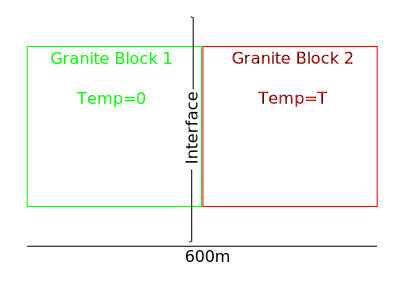
\includegraphics[width=4.in]{figures/onedheatdiff001}}
\caption{Example 1: Temperature differential along a single interface between
two granite blocks.}
\label{fig:onedgbmodel}
\end{figure}

\section{Example 1: One Dimensional Heat Diffusion in Granite}
\label{Sec:1DHDv00}

The first model consists of two blocks of isotropic material, for instance
granite, sitting next to each other.
Initial temperature in \textit{Block 1} is \verb|T1| and in \textit{Block 2} is
\verb|T2|.
We assume that the system is insulated.
What would happen to the temperature distribution in each block over time? 
Intuition tells us that heat will be transported from the hotter block to the
cooler one until both
blocks have the same temperature.

\subsection{1D Heat Diffusion Equation}
We can model the heat distribution of this problem over time using the one
dimensional heat diffusion equation\footnote{A detailed discussion on how the
heat diffusion equation is derived can be found at
\url{
http://online.redwoods.edu/instruct/darnold/DEProj/sp02/AbeRichards/paper.pdf}};
which is defined as:
\begin{equation}
\rho c\hackscore p \frac{\partial T}{\partial t} - \kappa \frac{\partial^{2}
T}{\partial x^{2}} = q\hackscore H 
\label{eqn:hd}
\end{equation}
where $\rho$ is the material density, $c\hackscore p$ is the specific heat and
$\kappa$ is the thermal 
conductivity\footnote{A list of some common thermal conductivities is available
from Wikipedia
\url{http://en.wikipedia.org/wiki/List_of_thermal_conductivities}}. Here we
assume that these material 
parameters are \textbf{constant}. 
The heat source is defined by the right hand side of \refEq{eqn:hd} as
$q\hackscore{H}$; this can take the form of a constant or a function of time and
space. For example $q\hackscore{H} = q\hackscore{0}e^{-\gamma t}$ where we have
the output of our heat source decaying with time. There are also two partial
derivatives in \refEq{eqn:hd}; $\frac{\partial T}{\partial t}$ describes the
change in temperature with time while $\frac{\partial ^2 T}{\partial x^2}$ is
the spatial change of temperature. As there is only a single spatial dimension
to our problem, our temperature solution $T$ is only dependent on the time $t$
and our signed distance from the block-block interface $x$.

\subsection{PDEs and the General Form}
It is possible to solve PDE \refEq{eqn:hd} analytically and obtain an exact
solution to our problem. However, it is not always practical to solve the
problem this way. Alternatively, computers can be used to find the solution. To
do this, a numerical approach is required to discretise 
the PDE \refEq{eqn:hd} across time and space, this reduces the problem to a
finite number of equations for a finite number of spatial points and time steps.
These parameters together define the model. While discretisation introduces
approximations and a degree of error, a sufficiently sampled model is generally
accurate enough to satisfy the accuracy requirements for the final solution.

Firstly, we discretise the PDE \refEq{eqn:hd} in time. This leaves us with a
steady linear PDE which involves spatial derivatives only and needs to be solved
in each time step to progress in time. \esc can help us here.

For time discretisation we use the Backward Euler approximation
scheme\footnote{see \url{http://en.wikipedia.org/wiki/Euler_method}}. It is
based on the approximation 
\begin{equation}
\frac{\partial T(t)}{\partial t} \approx \frac{T(t)-T(t-h)}{h}
\label{eqn:beuler}
\end{equation}
for  $\frac{\partial T}{\partial t}$  at time $t$ 
where $h$ is the time step size. This can also be written as;
\begin{equation}
\frac{\partial T}{\partial t}(t^{(n)}) \approx \frac{T^{(n)} - T^{(n-1)}}{h}
\label{eqn:Tbeuler}
\end{equation}
where the upper index $n$ denotes the n\textsuperscript{th} time step. So one
has
\begin{equation}
\begin{array}{rcl}
t^{(n)} & = & t^{(n-1)}+h \\
T^{(n)} & = & T(t^{(n-1)}) \\ 
\end{array}
\label{eqn:Neuler}
\end{equation}
Substituting \refEq{eqn:Tbeuler} into \refEq{eqn:hd} we get;
\begin{equation}
\frac{\rho c\hackscore p}{h} (T^{(n)} - T^{(n-1)}) - \kappa \frac{\partial^{2}
T^{(n)}}{\partial x^{2}} = q\hackscore H 
\label{eqn:hddisc}
\end{equation}
Notice that we evaluate the spatial derivative term at the current time
$t^{(n)}$ - therefore the name \textbf{backward Euler} scheme. Alternatively,
one can evaluate the spatial derivative term at the previous time $t^{(n-1)}$.
This approach is called the \textbf{forward Euler} scheme. This scheme can
provide some computational advantages, which
are not discussed here. However, the \textbf{forward Euler} scheme has a major
disadvantage. Namely, depending on the 
material parameters as well as the domain discretization of the spatial
derivative term, the time step size $h$ needs to be chosen sufficiently small to
achieve a stable temperature when progressing in time. Stability is achieved if
the temperature does not grow beyond its initial bounds and becomes
non-physical. 
The backward Euler scheme, which we use here, is unconditionally stable meaning
that under the assumption of a
physically correct problem set-up the temperature approximation remains physical
for all time steps. 
The user needs to keep in mind that the discretisation error introduced by
\refEq{eqn:beuler} 
is sufficiently small, thus a good approximation of the true temperature is
computed. It is therefore very important that any results are viewed with
caution. For example, one may compare the results for different time and
spatial step sizes.

To get the temperature $T^{(n)}$ at time $t^{(n)}$ we need to solve the linear 
differential equation \refEq{eqn:hddisc} which only includes spatial
derivatives. To solve this problem we want to use \esc. 

In \esc any given PDE can be described by the general form. For the purpose of
this introduction we illustrate a simpler version of the general form for full
linear PDEs which is available in the \esc user's guide. A simplified form that
suits our heat diffusion problem\footnote{The form in the \esc users guide which
uses the Einstein convention is written as 
$-(A\hackscore{jl} u\hackscore{,l})\hackscore{,j}+D u =Y$}
is described by;
\begin{equation}\label{eqn:commonform nabla}
-\nabla\cdot(A\cdot\nabla u) + Du = f
\end{equation}
where $A$, $D$ and $f$ are known values and $u$ is the unknown solution. The
symbol $\nabla$ which is called the \textit{Nabla operator} or \textit{del
operator} represents
the spatial derivative of its subject - in this case $u$. Lets assume for a
moment that we deal with a one-dimensional problem then ;
\begin{equation}
\nabla = \frac{\partial}{\partial x}
\end{equation}
and we can write \refEq{eqn:commonform nabla} as;
\begin{equation}\label{eqn:commonform}
-A\frac{\partial^{2}u}{\partial x^{2}} + Du = f
\end{equation}
if $A$ is constant. To match this simplified general form to our problem
\refEq{eqn:hddisc} 
we rearrange \refEq{eqn:hddisc};
\begin{equation}
\frac{\rho c\hackscore p}{h} T^{(n)} - \kappa \frac{\partial^2 T^{(n)}}{\partial
x^2} = q\hackscore H +  \frac{\rho c\hackscore p}{h} T^{(n-1)}
\label{eqn:hdgenf}
\end{equation}
The PDE is now in a form that satisfies \refEq{eqn:commonform nabla} which is
required for \esc to solve our PDE. This can be done by generating a solution
for successive increments in the time nodes $t^{(n)}$ where 
$t^{(0)}=0$ and  $t^{(n)}=t^{(n-1)}+h$ where $h>0$ is the step size and assumed
to be constant. 
In the following the upper index ${(n)}$ refers to a value at time $t^{(n)}$.
Finally, by comparing \refEq{eqn:hdgenf} with \refEq{eqn:commonform} one can see
that;
\begin{equation}\label{ESCRIPT SET}
u=T^{(n)}; 
A = \kappa; D = \frac{\rho c \hackscore{p}}{h}; f = q \hackscore{H} + \frac{\rho
c\hackscore p}{h} T^{(n-1)}
\end{equation}

\subsection{Boundary Conditions}
\label{SEC BOUNDARY COND}
With the PDE sufficiently modified, consideration must now be given to the
boundary conditions of our model. Typically there are two main types of boundary
conditions known as \textbf{Neumann} and \textbf{Dirichlet} boundary
conditions\footnote{More information on Boundary Conditions is available at
Wikipedia \url{http://en.wikipedia.org/wiki/Boundary_conditions}},
respectively. 
A \textbf{Dirichlet boundary condition} is conceptually simpler and is used to
prescribe a known value to the unknown solution (in our example the temperature)
on parts of the boundary or on the entire boundary of the region of interest. 
We discuss the Dirichlet boundary condition in our second example presented in
Section~\ref{Sec:1DHDv0}.

However, for this example we have made the model assumption that the system is
insulated, so we need to add an appropriate boundary condition to prevent
any loss or inflow of energy at the boundary of our domain. Mathematically this
is expressed by prescribing
the heat flux $\kappa \frac{\partial T}{\partial x}$  to zero. In our simplified
one dimensional model this is expressed
in the form;
\begin{equation}
\kappa \frac{\partial T}{\partial x}  = 0 
\end{equation}
or in a more general case as
\begin{equation}\label{NEUMAN 1}
\kappa \nabla T \cdot n  = 0 
\end{equation}
where $n$  is the outer normal field \index{outer normal field} at the surface
of the domain. 
The $\cdot$ (dot) refers to the dot product of the vectors $\nabla T$ and $n$.
In fact, the term $\nabla T \cdot n$ is the normal derivative of 
the temperature $T$. Other notations used here are\footnote{The \esc notation
for the normal
derivative is $T\hackscore{,i} n\hackscore i$.};
\begin{equation}
\nabla T \cdot n  = \frac{\partial T}{\partial n} \; .
\end{equation}
A condition of the type \refEq{NEUMAN 1} defines a \textbf{Neumann boundary
condition} for the PDE. 

The PDE \refEq{eqn:hdgenf} 
and the Neumann boundary condition~\ref{eqn:hdgenf} (potentially together with
the Dirichlet boundary conditions)  define a \textbf{boundary value problem}. 
It is the nature of a boundary value problem to allow making statements about
the solution in the
interior of the domain from information known on the boundary only. In most
cases we use the term partial differential equation but in fact it is a
boundary value problem. 
It is important to keep in mind that boundary conditions need to be complete and
consistent in the sense that 
at any point on the boundary either a Dirichlet or a Neumann boundary condition
must be set.

Conveniently, \esc makes a default assumption on the boundary conditions which
the user may modify where appropriate. 
For a problem of the form in~\refEq{eqn:commonform nabla} the default
condition\footnote{In the \esc user guide which uses the Einstein convention
this is written as 
$n\hackscore{j}A\hackscore{jl} u\hackscore{,l}=0$.} is;
\begin{equation}\label{NEUMAN 2}
-n\cdot A \cdot\nabla u = 0 
\end{equation}
which is used everywhere on the boundary. Again $n$ denotes the outer normal
field. 
Notice that the coefficient $A$ is the same as in the \esc
PDE~\ref{eqn:commonform nabla}. 
With the settings for the coefficients we have already identified in
\refEq{ESCRIPT SET} this
condition translates into 
\begin{equation}\label{NEUMAN 2b}
\kappa \frac{\partial T}{\partial x} = 0 
\end{equation}
for the boundary of the domain. This is identical to the Neumann boundary
condition we want to set. \esc will take care of this condition for us. We
discuss the Dirichlet boundary condition later.

\subsection{Outline of the Implementation}
\label{sec:outline}
To solve the heat diffusion equation (\refEq{eqn:hd}) we write a simple \pyt
script. At this point we assume that you have some basic understanding of the
\pyt programming language. If not, there are some pointers and links available
in Section \ref{sec:escpybas}. The script (discussed in \refSec{sec:key}) has
four major steps. Firstly, we need to define the domain where we want to 
calculate the temperature. For our problem this is the joint blocks of granite
which has a rectangular shape. Secondly, we need to define the PDE to solve in
each time step to get the updated temperature. Thirdly, we need to define the
coefficients of the PDE and finally we need to solve the PDE. The last two steps
need to be repeated until the final time marker has been reached. The work flow
is described in \reffig{fig:wf}.
% \begin{enumerate}
%  \item create domain
%  \item create PDE
%  \item while end time not reached:
% \begin{enumerate}
%  \item set PDE coefficients
%  \item solve PDE
%  \item update time marker
% \end{enumerate}
% \item end of calculation
% \end{enumerate}

\begin{figure}[h!]
 \centering
   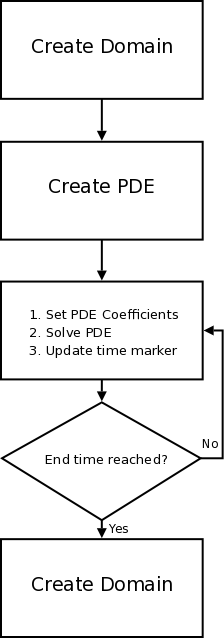
\includegraphics[width=1in]{figures/workflow.png}
   \caption{Workflow for developing an \esc model and solution}
   \label{fig:wf}
\end{figure}

In the terminology of \pyt, the domain and PDE are represented by
\textbf{objects}. The nice feature of an object is that it is defined by its
usage and features
rather than its actual representation. So we will create a domain object to
describe the geometry of the two
granite blocks. Then we define PDEs and spatially distributed values such as the
temperature 
on this domain. Similarly, to define a PDE object we use the fact that one needs
only to define the coefficients of the PDE and solve the PDE. The PDE object has
advanced features, but these are not required in simple cases.


\begin{figure}[t]
 \centering
   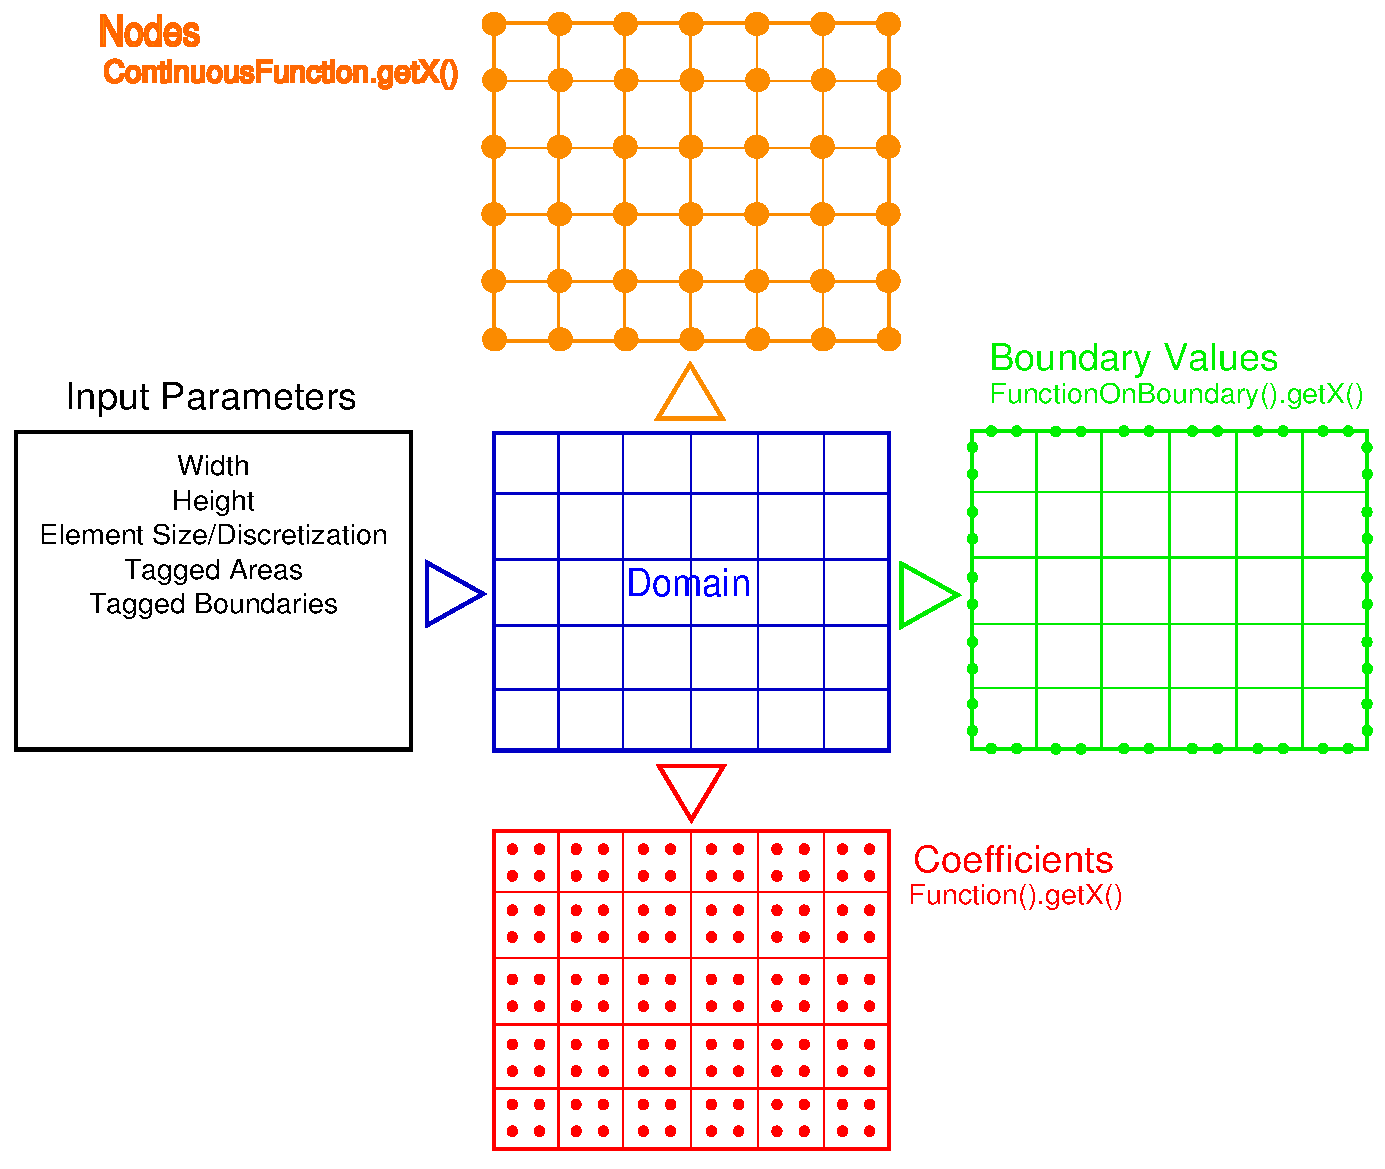
\includegraphics[width=6in]{figures/functionspace.pdf}
   \caption{\esc domain construction overview}
   \label{fig:fs}
\end{figure}

\subsection{The Domain Constructor in \esc}
\label{ss:domcon}
Whilst it is not strictly relevant or necessary, a better understanding of
how values are spatially distributed (\textit{e.g.} Temperature) and how PDE
coefficients are interpreted in \esc can be helpful.

There are various ways to construct domain objects. The simplest form is a
rectangular shaped region with a length and height. There is
a ready to use function for this named \verb rectangle(). Besides the spatial
dimensions this function requires to specify the number of
elements or cells to be used along the length and height, see \reffig{fig:fs}.
Any spatially distributed value 
and the PDE is represented in discrete form using this element
representation\footnote{We use the finite element method (FEM), see
\url{http://en.wikipedia.org/wiki/Finite_element_method} for details.}.
Therefore we will have access to an approximation of the true PDE solution
only. 
The quality of the approximation depends - besides other factors - mainly on the
number of elements being used. In fact, the 
approximation becomes better when more elements are used. However, computational
cost grows with the number of
elements being used. It is therefore important that you find the right balance
between the demand in accuracy and acceptable resource usage.

In general, one can think about a domain object as a composition of nodes and
elements. 
As shown in \reffig{fig:fs}, an element is defined by the nodes that are used to
describe its vertices. 
To represent spatially distributed values the user can use 
the values at the nodes, at the elements in the interior of the domain or at the
elements located on the surface of the domain. 
The different approach used to represent values is called \textbf{function
space} and is attached to all objects
in \esc representing a spatially distributed value such as the solution of
a PDE. The three function spaces we use at the moment are;
\begin{enumerate}
\item the nodes, called by \verb|ContinuousFunction(domain)| ;
\item the elements/cells, called by \verb|Function(domain)| ; and
\item the boundary, called by \verb|FunctionOnBoundary(domain)|.
\end{enumerate}
A function space object such as \verb|ContinuousFunction(domain)| has the method
\verb|getX| attached to it. This method returns the
location of the so-called \textbf{sample points} used to represent values of the
particular function space. So the
call \verb|ContinuousFunction(domain).getX()| will return the coordinates of the
nodes used to describe the domain while
\verb|Function(domain).getX()| returns the coordinates of numerical
integration points within elements, see \reffig{fig:fs}. 

This distinction between different representations of spatially distributed
values 
is important in order to be able to vary the degrees of smoothness in a PDE
problem. 
The coefficients of a PDE do not need to be continuous, thus this qualifies as a
\verb|Function()| type. 
On the other hand a temperature distribution must be continuous and needs to be
represented with a \verb|ContinuousFunction()| function space.
An influx may only be defined at the boundary and is therefore a
\verb|FunctionOnBoundary()| object.  
\esc allows certain transformations of the function spaces. A
\verb|ContinuousFunction()| can be transformed into a
\verb|FunctionOnBoundary()| or \verb|Function()|. On the other hand there is
not enough information in a \verb|FunctionOnBoundary()| to transform it to a
\verb|ContinuousFunction()|.
These transformations, which are called \textbf{interpolation} are invoked
automatically by \esc if needed.

Later in this introduction we discuss how
to define specific areas of geometry with different materials which are
represented by different material coefficients such as the
thermal conductivities $\kappa$. A very powerful technique to define these types
of PDE 
coefficients is tagging. Blocks of materials and boundaries can be named and
values can be defined on subregions based on their names.
This is a method for simplifying PDE coefficient and flux definitions. It makes
scripting much easier and we will discuss this technique in
Section~\ref{STEADY-STATE HEAT REFRACTION}.


\subsection{A Clarification for the 1D Case}
\label{SEC: 1D CLARIFICATION}
It is necessary for clarification that we revisit our general PDE from
\refeq{eqn:commonform nabla} for a two dimensional domain. \esc is inherently
designed to solve problems that are multi-dimensional and so
\refEq{eqn:commonform nabla} needs to be read as a higher dimensional problem.
In the case of two spatial dimensions the \textit{Nabla operator} has in fact
two components $\nabla = (\frac{\partial}{\partial x}, \frac{\partial}{\partial
y})$. Assuming the coefficient $A$ is constant, the \refEq{eqn:commonform nabla}
takes the following form;
\begin{equation}\label{eqn:commonform2D}
-A\hackscore{00}\frac{\partial^{2}u}{\partial x^{2}} 
-A\hackscore{01}\frac{\partial^{2}u}{\partial x\partial y} 
-A\hackscore{10}\frac{\partial^{2}u}{\partial y\partial x} 
-A\hackscore{11}\frac{\partial^{2}u}{\partial y^{2}} 
+ Du = f
\end{equation}
Notice that for the higher dimensional case $A$ becomes a matrix. It is also
important to notice that the usage of the Nabla operator creates
a compact formulation which is also independent from the spatial dimension. 
To make the general PDE \refEq{eqn:commonform2D} one dimensional as
shown in \refEq{eqn:commonform} we need to set
\begin{equation}
A\hackscore{00}=A; A\hackscore{01}=A\hackscore{10}=A\hackscore{11}=0
\end{equation}


\subsection{Developing a PDE Solution Script}
\label{sec:key}
\sslist{example01a.py}
We write a simple \pyt script which uses the \modescript, \modfinley and \modmpl
modules. 
By developing a script for \esc, the heat diffusion equation can be solved at
successive time steps for a predefined period using our general form
\refEq{eqn:hdgenf}. Firstly it is necessary to import all the
libraries\footnote{The libraries contain predefined scripts that are required to
solve certain problems, these can be simple like sine and cosine functions or
more complicated like those from our \esc library.} 
that we will require.
\begin{python}
from esys.escript import *
# This defines the LinearPDE module as LinearPDE
from esys.escript.linearPDEs import LinearPDE 
# This imports the rectangle domain function from finley.
from esys.finley import Rectangle 
# A useful unit handling package which will make sure all our units
# match up in the equations under SI.
from esys.escript.unitsSI import * 
\end{python}
It is generally a good idea to import all of the \modescript library, although
if the functions and classes required are known they can be specified
individually. The function \verb|LinearPDE| has been imported explicitly for
ease of use later in the script. \verb|Rectangle| is going to be our type of
domain. The module \verb|unitsSI| provides support for SI unit definitions with
our variables.

Once our library dependencies have been established, defining the problem
specific variables is the next step. In general the number of variables needed
will vary between problems. These variables belong to two categories. They are
either directly related to the PDE and can be used as inputs into the \esc
solver, or they are script variables used to control internal functions and
iterations in our problem. For this PDE there are a number of constants which
need values. Firstly, the domain upon which we wish to solve our problem needs
to be defined. There are different types of domains in \modescript which we
demonstrate in later tutorials but for our granite blocks, we simply use a
rectangular domain. 

Using a rectangular domain simplifies our granite blocks (which would in reality
be a \textit{3D} object) into a single dimension. The granite blocks will have a
lengthways cross section that looks like a rectangle.  As a result we do not
need to model the volume of the block due to symmetry. There are four arguments
we must consider when we decide to create a rectangular domain, the domain
\textit{length}, \textit{width} and \textit{step size} in each direction. When
defining the size of our problem it will help us determine appropriate values
for our model arguments. If we make our dimensions large but our step sizes very
small we increase the accuracy of our solution. Unfortunately we also increase
the number of calculations that must be solved per time step. This means more
computational time is required to produce a solution. In this \textit{1D}
problem, the bar is defined as being 1 metre long. An appropriate step size
\verb|ndx| would be 1 to 10\% of the length. Our \verb|ndy| needs only be 1,
this is because our problem stipulates no partial derivatives in the $y$
direction.
Thus the temperature does not vary with $y$. Hence, the model parameters can be
defined as follows; note we have used the \verb|unitsSI| convention to make sure
all our input units are converted to SI.
\begin{python}
mx = 500.*m #meters - model length
my = 100.*m #meters - model width
ndx = 50 # mesh steps in x direction 
ndy = 1 # mesh steps in y direction
boundloc = mx/2 # location of boundary between the two blocks
\end{python}
The material constants and the temperature variables must also be defined. For
the granite in the model they are defined as:
\begin{python}
#PDE related
rho = 2750. *kg/m**3 #kg/m^{3} density of iron
cp = 790.*J/(kg*K) # J/Kg.K thermal capacity
rhocp = rho*cp 
kappa = 2.2*W/m/K   # watts/m.Kthermal conductivity
qH=0 * J/(sec*m**3) # J/(sec.m^{3}) no heat source
T1=20 * Celsius # initial temperature at Block 1
T2=2273. * Celsius # base temperature at Block 2
\end{python}
Finally, to control our script we will have to specify our timing controls and
where we would like to save the output from the solver. This is simple enough:
\begin{python}
t=0 * day  #our start time, usually zero
tend=1. * day # - time to end simulation
outputs = 200 # number of time steps required.
h=(tend-t)/outputs #size of time step
#user warning statement
print "Expected Number of time outputs is: ", (tend-t)/h
i=0 #loop counter
\end{python}
Now that we know our inputs we will build a domain using the
\verb|Rectangle()| function from \FINLEY. The four arguments allow us to
define our domain \verb|model| as:
\begin{python}
#generate domain using rectangle
blocks = Rectangle(l0=mx,l1=my,n0=ndx, n1=ndy)
\end{python}
\verb|blocks| now describes a domain in the manner of Section \ref{ss:domcon}.

With a domain and all the required variables established, it is now possible to
set up our PDE so that it can be solved by \esc. The first step is to define the
type of PDE that we are trying to solve in each time step. In this example it is
a single linear PDE\footnote{in contrast to a system of PDEs which we discuss
later.}. We also need to state the values of our general form variables.
\begin{python}
mypde=LinearPDE(blocks)
A=zeros((2,2)))
A[0,0]=kappa
mypde.setValue(A=A, D=rhocp/h)
\end{python}
In many cases it may be possible to decrease the computational time of the
solver if the PDE is symmetric. 
Symmetry of a PDE is defined by;
\begin{equation}\label{eqn:symm}
A\hackscore{jl}=A\hackscore{lj}
\end{equation}
Symmetry is only dependent on the $A$ coefficient in the general form and the
other coefficients $D$ as well as the right hand side $Y$. From the above
definition we can see that our PDE is symmetric. The \verb|LinearPDE| class
provides the method \method{checkSymmetry} to check if the given PDE is
symmetric. As our PDE is symmetrical we enable symmetry via;
\begin{python}
myPDE.setSymmetryOn()
\end{python}
Next we need to establish the initial temperature distribution \verb|T|. We need
to 
assign the value \verb|T1| to all sample points left to the contact interface at
$x\hackscore{0}=\frac{mx}{2}$
and the value \verb|T2| right to the contact interface. \esc
provides the \verb|whereNegative| function to construct this. More
specifically, \verb|whereNegative| returns the value $1$ at those sample points
where the argument has a negative value. Otherwise zero is returned.
If \verb|x| are the $x\hackscore{0}$ 
coordinates of the sample points used to represent the temperature distribution 
then \verb|x[0]-boundloc| gives us a negative value for 
all sample points left to the interface and non-negative value to 
the right of the interface. So with;
\begin{python}
# ... set initial temperature ....
T= T1*whereNegative(x[0]-boundloc)+T2*(1-whereNegative(x[0]-boundloc))
\end{python}
we get the desired temperature distribution. To get the actual sample points
\verb|x| we use the \verb|getX()| method of the function space
\verb|Solution(blocks)| which is used to represent the solution of a PDE;
\begin{python}
x=Solution(blocks).getX()
\end{python}
As \verb|x| are the sample points for the function space
\verb|Solution(blocks)| 
the initial temperature \verb|T| is using these sample points for
representation.
Although \esc is trying to be forgiving with the choice of sample points and to
convert
where necessary the adjustment of the function space is not always possible. So
it is advisable to make a careful choice on the function space used.  

Finally we initialise an iteration loop to solve our PDE for all the time steps
we specified in the variable section. As the right hand side of the general form
is dependent on the previous values for temperature \verb T  across the bar this
must be updated in the loop. Our output at each time step is \verb T  the heat
distribution and \verb totT  the total heat in the system.
\begin{python}
while t < tend:
	i+=1 #increment the counter
	t+=h #increment the current time
	mypde.setValue(Y=qH+rhocp/h*T) # set variable PDE coefficients
	T=mypde.getSolution() #get the PDE solution
	totE = integrate(rhocp*T) #get the total heat (energy) in the system
\end{python}
The last statement in this script calculates the total energy in the system as
the volume integral of $\rho c\hackscore{p} T$ over the block.
As the blocks are insulated no energy should be lost or added. 
The total energy should stay constant for the example discussed here.

\subsection{Running the Script} 
The script presented so far is available under 
\verb|example01a.py|. You can edit this file with your favourite text editor. 
On most operating systems\footnote{The \texttt{run-escript} launcher is not
supported under {\it MS Windows} yet.} you can use the
\program{run-escript} command 
to launch {\it escript} scripts. For the example script use;
\begin{verbatim}
run-escript example01a.py
\end{verbatim}
The program will print a progress report. Alternatively, you can use 
the python interpreter directly;
\begin{verbatim}
python example01a.py
\end{verbatim}
if the system is configured correctly (please talk to your system
administrator).

\begin{figure}
\begin{center}
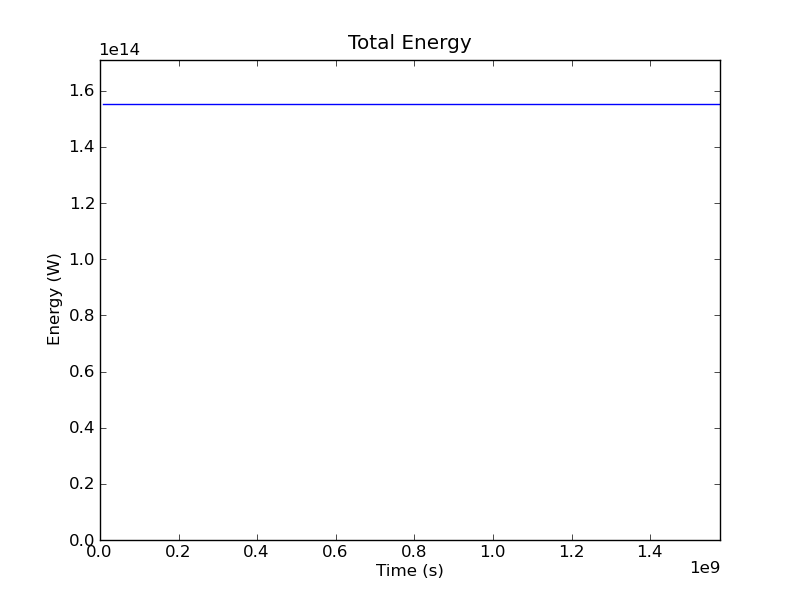
\includegraphics[width=4in]{figures/ttblockspyplot150}
\caption{Example 1b: Total Energy in the Blocks over Time (in seconds)}
\label{fig:onedheatout1} 
\end{center}
\end{figure}

\subsection{Plotting the Total Energy} 
\sslist{example01b.py}

\esc does not include its own plotting capabilities. However, it is possible to
use a variety of free \pyt packages for visualisation.
Two types will be demonstrated in this cookbook;
\mpl\footnote{\url{http://matplotlib.sourceforge.net/}} and 
\verb|VTK|\footnote{\url{http://www.vtk.org/}}. 
The \mpl package is a component of SciPy\footnote{\url{http://www.scipy.org}}
and is good for basic graphs and plots. 
For more complex visualisation tasks, in particular two and three dimensional
problems we recommend the use of more advanced tools. For instance,  \mayavi
\footnote{\url{http://code.enthought.com/projects/mayavi/}}
which is based upon the \verb|VTK| toolkit. The usage of \verb|VTK| based 
visualisation is discussed in Chapter~\ref{Sec:2DHD} which focuses on a two
dimensional PDE. 

For our simple granite block problem, we have two plotting tasks. Firstly, we
are interested in showing the
behaviour of the total energy over time and secondly, how the temperature
distribution within the block is developing over time.
Let us start with the first task.

The idea is to create a record of the time marks and the corresponding total
energies observed.
\pyt provides the concept of lists for this. Before 
the time loop is opened we create empty lists for the time marks \verb|t_list|
and the total energies \verb|E_list|. 
After the new temperature has been calculated by solving the PDE we append the
new time marker and the total energy value for that time
to the corresponding list using the \verb|append| method. With these
modifications our script looks as follows:
\begin{python}
t_list=[]
E_list=[]
# ... start iteration:
while t<tend:
      t+=h
      mypde.setValue(Y=qH+rhocp/h*T) # set variable PDE coefficients
      T=mypde.getSolution() #get the PDE solution
      totE=integrate(rhocp*T) 
      t_list.append(t)   # add current time mark to record
      E_list.append(totE) # add current total energy to record
\end{python}
To plot $t$ over $totE$ we use \mpl a module contained within \pylab which needs
to be loaded before use;
\begin{python}
import pylab as pl # plotting package.
\end{python}
Here we are not using \verb|from pylab import *| in order to avoid name
clashes for function names within \esc. 

The following statements are added to the script after the time loop has been
completed;
\begin{python}
pl.plot(t_list,E_list)
pl.title("Total Energy")
pl.axis([0,max(t_list),0,max(E_list)*1.1])
pl.savefig("totE.png")
\end{python}
The first statement hands over the time marks and corresponding total energies
to the plotter.
The second statement sets the title for the plot. The third statement
sets the axis ranges. In most cases these are set appropriately by the plotter.
 
The last statement generates the plot and writes the result into the file
\verb|totE.png| which can be displayed by (almost) any image viewer. 
As expected the total energy is constant over time, see
\reffig{fig:onedheatout1}.

\subsection{Plotting the Temperature Distribution}
\label{sec: plot T}
\sslist{example01c.py}
For plotting the spatial distribution of the temperature we need to modify the
strategy we have used for the total energy.
Instead of producing a final plot at the end we will generate a 
picture at each time step which can be browsed as a slide show or composed into
a movie.
The first problem we encounter is that if we produce an image at each time step
we need to make sure that the images previously generated are not overwritten.

To develop an incrementing file name we can use the following convention. It is
convenient to put all image files showing the same variable - in our case the
temperature distribution - into a separate directory.
As part of the \verb|os| module\footnote{The \texttt{os} module provides 
a powerful interface to interact with the operating system, see
\url{http://docs.python.org/library/os.html}.} \pyt 
provides the \verb|os.path.join| command to build file and directory names in a
platform independent way. Assuming that 
\verb|save_path| is the name of the directory we want to put the results in the
command is; 
\begin{python}
import os
os.path.join(save_path, "tempT%03d.png"%i )
\end{python}
where \verb|i| is the time step counter.
There are two arguments to the \verb|join| command. The \verb|save_path|
variable is a predefined string pointing to the directory we want to save our
data, for example a single sub-folder called \verb|data| would be defined by;
\begin{verbatim}
save_path = "data"
\end{verbatim}
while a sub-folder of \verb|data| called \verb|example01| would be defined by;
\begin{verbatim}
save_path = os.path.join("data","example01")
\end{verbatim}
The second argument of \verb|join| contains a string which is the file
name or subdirectory name. We can use the operator \verb|%| to use the value of
\verb|i| as part of our filename. The sub-string \verb|%03d| indicates that we
want to substitute a value into the name; 
\begin{itemize}
 \item \verb 0  means that small numbers should have leading zeroes;
 \item \verb 3  means that numbers should be written using at least 3 digits;
and
 \item \verb d  means that the value to substitute will be a decimal integer.
\end{itemize}
To actually substitute the value of \verb|i| into the name write \verb|%i| after
the string.
When done correctly, the output files from this command will be placed in the
directory defined by \verb save_path  as;
\begin{verbatim}
blockspyplot001.png
blockspyplot002.png
blockspyplot003.png
...
\end{verbatim}
and so on.

A sub-folder check/constructor is available in \esc. The command;
\begin{verbatim}
mkDir(save_path)
\end{verbatim}
will check for the existence of \verb save_path  and if missing, create the
required directories.

We start by modifying our solution script.
Prior to the \verb|while| loop we need to extract our finite solution
points to a data object that is compatible with \mpl. First we create the node
coordinates of the sample points used to represent
the temperature as a \pyt list of tuples or a \numpy array as requested by the
plotting function. 
We need to convert the array \verb|x| previously set as
\verb|Solution(blocks).getX()| into a \pyt list 
and then to a \numpy array. The $x\hackscore{0}$ component is then extracted via
an array slice to the variable \verb|plx|; 
\begin{python}
import numpy as np # array package.
#convert solution points for plotting
plx = x.toListOfTuples() 
plx = np.array(plx) # convert to tuple to numpy array
plx = plx[:,0] # extract x locations
\end{python}

\begin{figure}
\begin{center}
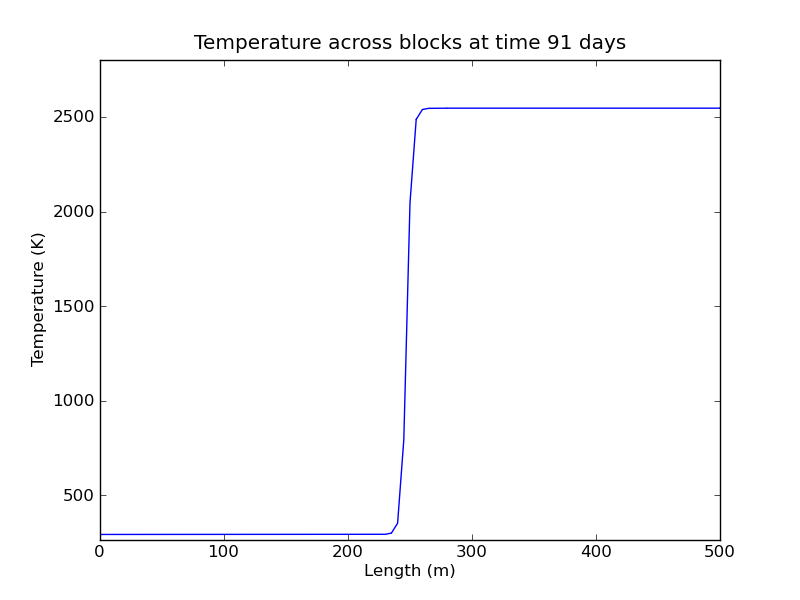
\includegraphics[width=4in]{figures/blockspyplot001}
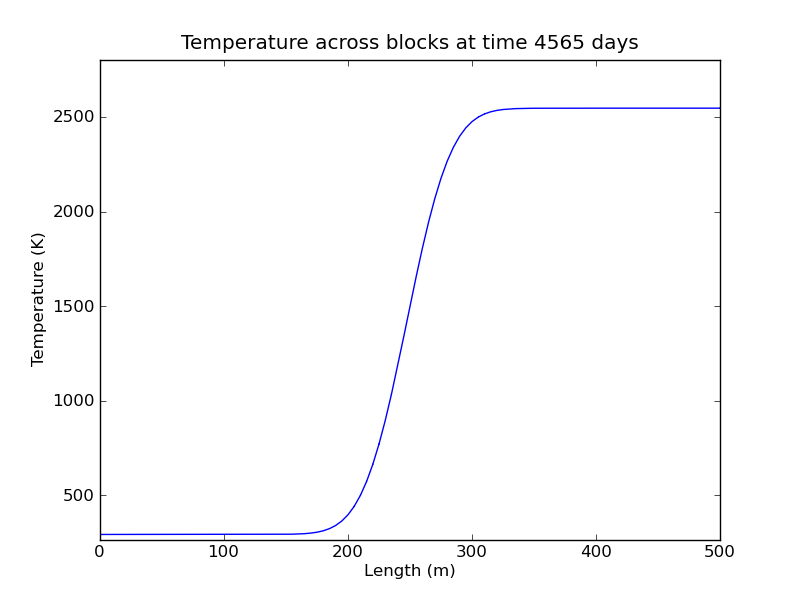
\includegraphics[width=4in]{figures/blockspyplot050}
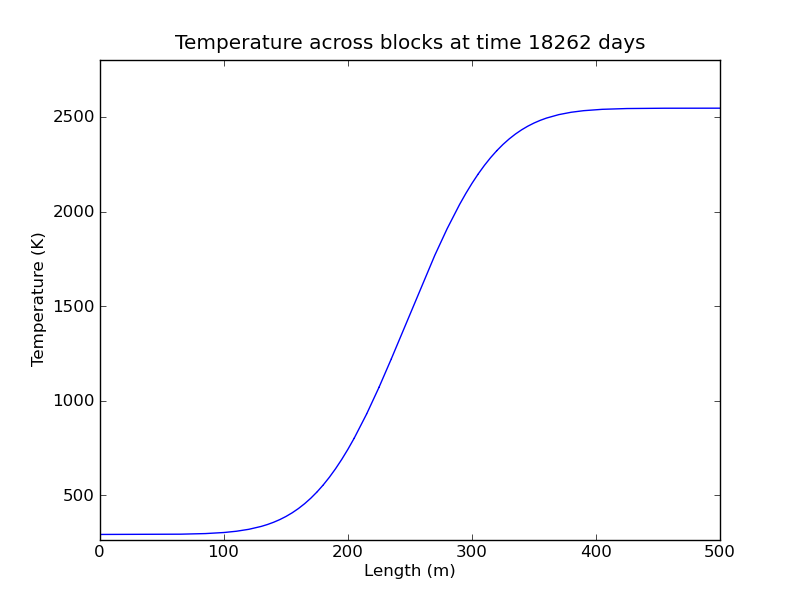
\includegraphics[width=4in]{figures/blockspyplot200}
\caption{Example 1c: Temperature ($T$) distribution in the blocks at time steps
$1$, $50$ and $200$}
\label{fig:onedheatout} 
\end{center}
\end{figure}

We use the same techniques provided by \mpl as we have used to plot the total
energy over time. 
For each time step we generate a plot of the temperature distribution and save
each to a file. 
The following is appended to the end of the \verb|while| loop and creates one
figure of the temperature distribution. We start by converting the solution to a
tuple and then plotting this against our \textit{x coordinates} \verb|plx| we
have generated before. We add a title to the diagram before it is rendered into
a file. 
Finally, the figure is saved to a \verb|*.png| file and cleared for the
following iteration.
\begin{python}
# ... start iteration:
while t<tend:
        ....
	T=mypde.getSolution() #get the PDE solution
        tempT = T.toListOfTuples() # convert to a tuple
        pl.plot(plx,tempT) # plot solution
	# set scale (Temperature should be between Tref and T0)
        pl.axis([0,mx,Tref*.9,T0*1.1])
        # add title
	pl.title("Temperature across the blocks at time %e minutes"%(t/day))
	#save figure to file
	pl.savefig(os.path.join(save_path,"tempT","blockspyplot%03d.png") %i)
\end{python}
Some results are shown in \reffig{fig:onedheatout}. 

\subsection{Making a Video} 
Our saved plots from the previous section can be cast into a video using the
following command appended to the end of the script. The \verb mencoder command
is not available on every platform, so some users need to use an alternative
video encoder.
\begin{python}
# compile the *.png files to create a *.avi video that shows T change
# with time. This operation uses Linux mencoder. For other operating 
# systems it is possible to use your favourite video compiler to
# convert image files to videos.

os.system("mencoder mf://"+save_path+"/tempT"+"/*.png -mf type=png:\
           w=800:h=600:fps=25 -ovc lavc -lavcopts vcodec=mpeg4 -oac copy -o \
           example01tempT.avi")
\end{python}
 

 
%%%%%%%%%%%%%%%%%%%%%%%%%%%%%%%%%%%%%%%%%%%%%%%%%%%%%%%%
%
% Copyright (c) 2003-2010 by University of Queensland
% Earth Systems Science Computational Center (ESSCC)
% http://www.uq.edu.au/esscc
%
% Primary Business: Queensland, Australia
% Licensed under the Open Software License version 3.0
% http://www.opensource.org/licenses/osl-3.0.php
%
%%%%%%%%%%%%%%%%%%%%%%%%%%%%%%%%%%%%%%%%%%%%%%%%%%%%%%%%
\begin{figure}[ht]
\centerline{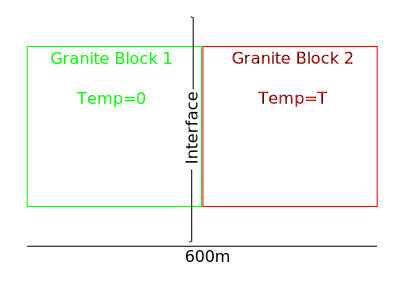
\includegraphics[width=4.in]{figures/onedheatdiff002}}
\caption{Example 2: One dimensional model of an Iron bar.}
\label{fig:onedhdmodel}
\end{figure}

\section{Example 2: One Dimensional Heat Diffusion in an Iron Rod}
\sslist{example02.py}
\label{Sec:1DHDv0}

Our second example is a cold iron bar at a constant temperature of $T\hackscore{ref}=20^{\circ} C$, see \reffig{fig:onedhdmodel}. The bar is perfectly insulated on all sides with a heating element at one end keeping the the temperature at a constant level $T\hackscore0=100^{\circ} C$.  As heat is applied; energy will disperse along the bar via conduction. With time the bar will reach a constant temperature equivalent to that of the heat source.

This problem is very similar to the example of temperature diffusion in granite blocks presented in the previous section~\ref{Sec:1DHDv00}. So we modify the script we have already developed for the granite blocks to adjust 
it to the iron bar problem.  
The obvious difference between the two problems are the dimensions of the domain and different materials involved. This will change the time scale of the model from years to hours. 
The new settings are;
\begin{python}
#Domain related.
mx = 1*m #meters - model length
my = .1*m #meters - model width
ndx = 100 # mesh steps in x direction 
ndy = 1 # mesh steps in y direction - one dimension means one element
#PDE related
rho = 7874. *kg/m**3 #kg/m^{3} density of iron
cp = 449.*J/(kg*K) # J/Kg.K thermal capacity
rhocp = rho*cp 
kappa = 80.*W/m/K   # watts/m.Kthermal conductivity
qH = 0 * J/(sec*m**3) # J/(sec.m^{3}) no heat source
Tref = 20 * Celsius  # base temperature of the rod
T0 = 100 * Celsius # temperature at heating element
tend= 0.5 * day # - time to end simulation
\end{python}
We also need to alter the initial value for the temperature. Now we need to set the 
temperature to $T\hackscore{0}$ at the left end of the rod where we have $x\hackscore{0}=0$ and 
$T\hackscore{ref}$ elsewhere. Instead of \verb|whereNegative| function we use now the 
\verb|whereZero| which returns the value one for those sample points where 
the argument (almost) equals zero and the value zero elsewhere. The initial
temperature is set to;
\begin{python}
# ... set initial temperature ....
T= T0*whereZero(x[0])+Tref*(1-whereZero(x[0]))
\end{python}

\subsection{Dirichlet Boundary Conditions}
In iron rod model  we want to keep the initial temperature $T\hackscore0$ on the left side of the domain over time. 
So when we solve the PDE~\refEq{eqn:hddisc} the solution must have the value $T\hackscore0$ on the left hand
side of the domain. As mentioned already in Section~\ref{SEC BOUNDARY COND} where we discussed
boundary condition this kind of condition are called a \textbf{Dirichlet boundary condition}. Some people also
use the term \textbf{constraint} for the PDE. 

To define a Dirichlet boundary condition we need to define where to apply the condition and what value the 
solution should have at these locations. In \esc we use $q$ and $r$ to define the Dirichlet boundary conditions
for a PDE. The solution $u$ of the PDE is set to $r$ for all sample points where $q$ has a positive value.
Mathematically this is expressed in the form;
\begin{equation}
  u(x) = r(x) \mbox{ for any } x \mbox{ with } q(x) > 0
\end{equation} 
In the case of the iron rod 
we can set;
\begin{python}
q=whereZero(x[0])
r=T0
\end{python}
to prescribe the value $T0$ for the temperature at the left end of the rod where $x\hackscore{0}=0$. 
Here we use the \verb|whereZero| function again which we have already used to set the initial value.
Notice that $r$ is set to the constant value $r$ for all sample points. In fact, 
values of $r$ are used only where $q$ is positive. Where $q$ is non-positive,
$r$ may have any value as these values are not used by the PDE solver. 

To set the Dirichlet boundary conditions for the PDE to be solved in each time step we need
to add some statements;
\begin{python}
mypde=LinearPDE(rod)
A=zeros((2,2)))
A[0,0]=kappa
q=whereZero(x[0])
mypde.setValue(A=A, D=rhocp/h, q=q, r=T0)
\end{python}
It is important to remark here that the Dirichlet condition \textbf{overwrites} any Neuman boundary 
condition \esc sets by default (or you may set).  

\begin{figure}
\begin{center}
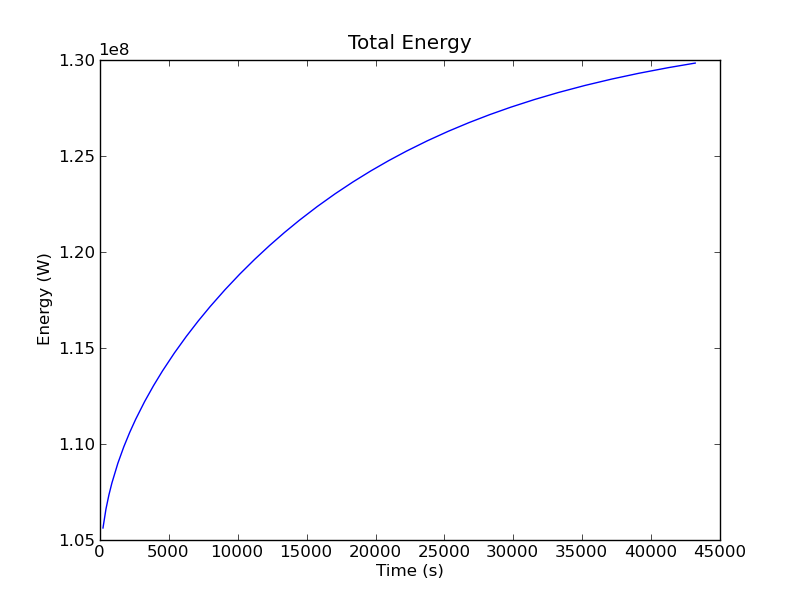
\includegraphics[width=4in]{figures/ttrodpyplot150}
\caption{Example 2: Total Energy in the Iron Rod over Time (in seconds).}
\label{fig:onedheatout1 002} 
\end{center}
\end{figure}

\begin{figure}
\begin{center}
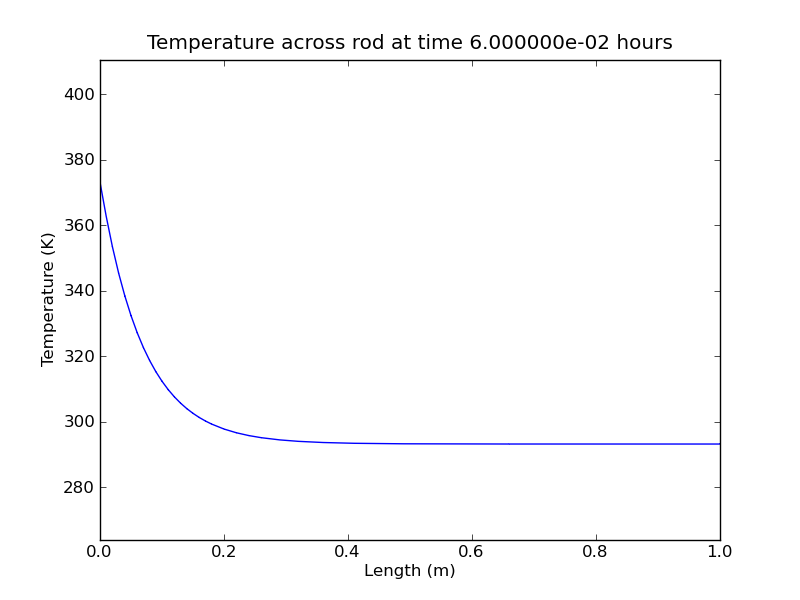
\includegraphics[width=4in]{figures/rodpyplot001}
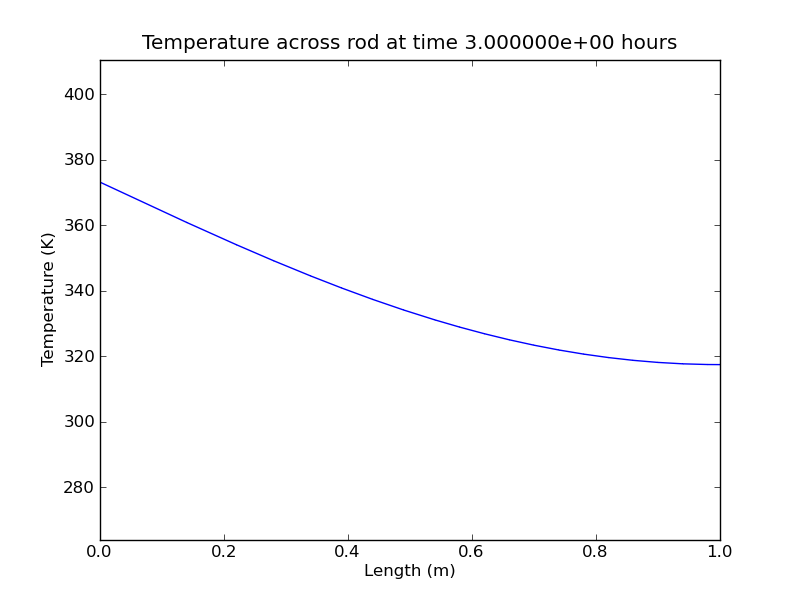
\includegraphics[width=4in]{figures/rodpyplot050}
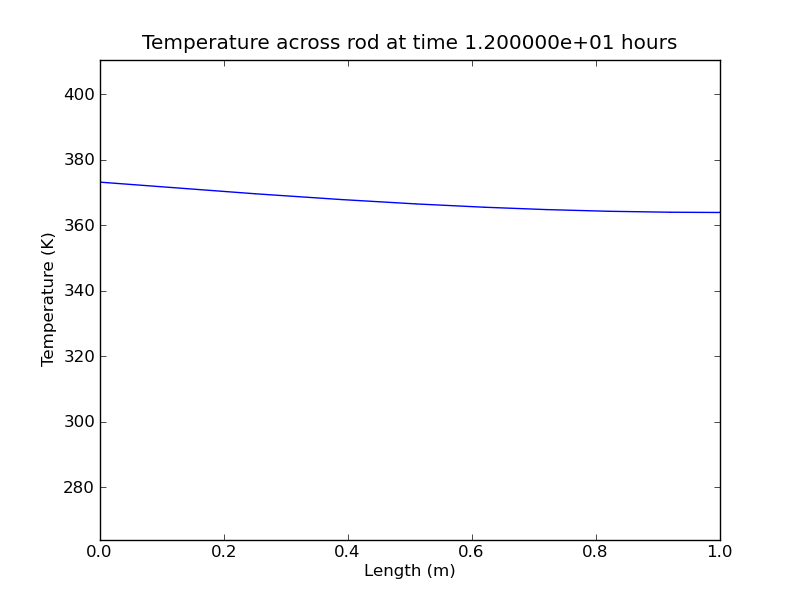
\includegraphics[width=4in]{figures/rodpyplot200}
\caption{Example 2: Temperature ($T$) distribution in the iron rod at time steps $1$, $50$ and $200$.}
\label{fig:onedheatout 002} 
\end{center}
\end{figure}

Besides some cosmetic modification this all we need to change. The total energy over time is shown in \reffig{fig:onedheatout1 002}. As heat
is transfered into the rod by the heater the total energy is growing over time but reaches a plateau 
when the temperature is constant is the rod, see \reffig{fig:onedheatout 002}. 
You will notice that the time scale of this model is several order of magnitudes faster than
for the granite rock problem due to the different length scale and material parameters. 
In practice it can take a few models run before the right time scale has been chosen\footnote{An estimate of the
time scale for a diffusion problem is given by the formula $\frac{\rho c\hackscore{p} L\hackscore{0}^2}{4 \kappa}$, see
\url{http://en.wikipedia.org/wiki/Fick\%27s_laws_of_diffusion}}.






\section{For the Reader}
\begin{enumerate}
 \item Move the boundary line between the two granite blocks to another part of the domain.
 \item Split the domain into multiple granite blocks with varying temperatures.
 \item Vary the mesh step size. Do you see a difference in the answers? What does happen with the compute time?
 \item Insert an internal heat source (Hint: The internal heat source is given by $q\hackscore{H}$.)
 \item Change the boundary condition for iron rod example such that the temperature 
 at the right end is kept at a constant level $T\hackscore{ref}$, which corresponds to the installation of a cooling element (Hint: Modify $q$ and $r$). 
\end{enumerate}


 % % % 
\chapter{Heat Diffusion in Two Dimensions}
 \label{CHAP HEAT 2a}
 
%%%%%%%%%%%%%%%%%%%%%%%%%%%%%%%%%%%%%%%%%%%%%%%%%%%%%%%%
%
% Copyright (c) 2003-2011 by University of Queensland
% Earth Systems Science Computational Center (ESSCC)
% http://www.uq.edu.au/esscc
%
% Primary Business: Queensland, Australia
% Licensed under the Open Software License version 3.0
% http://www.opensource.org/licenses/osl-3.0.php
%
%%%%%%%%%%%%%%%%%%%%%%%%%%%%%%%%%%%%%%%%%%%%%%%%%%%%%%%%

\begin{figure}[t]
\centerline{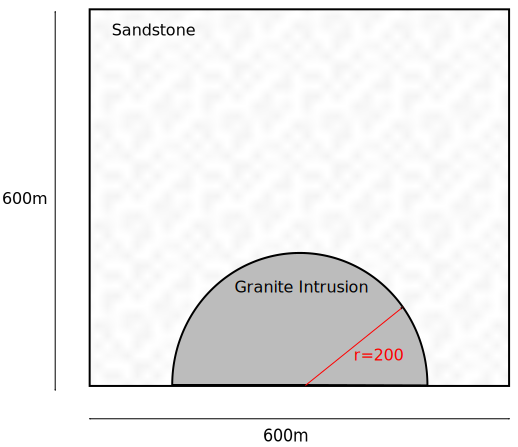
\includegraphics[width=4.in]{figures/twodheatdiff}}
\caption{Example 3: 2D model: granitic intrusion of sandstone country rock}
\label{fig:twodhdmodel}
\end{figure}

\sslist{example03a.py and cblib.py}

Building upon our success from the 1D models, it is now prudent to expand our
domain by another dimension. 
For this example we use a very simple magmatic intrusion as the basis for our
model. The simulation will be a single event where some molten granite has
formed a cylindrical dome at the base of some cold sandstone country rock.
Assuming that the cylinder is very long
we model a cross-section as shown in \reffig{fig:twodhdmodel}. We will implement
the same 
diffusion model as we have used for the granite blocks in \refSec{Sec:1DHDv00}
but will add the second spatial dimension and show how to define 
variables depending on the location of the domain. 
We use \file{onedheatdiff001b.py} as the starting point to develop this model. 

\section{Example 3: Two Dimensional Heat Diffusion for a basic Magmatic
Intrusion}
\label{Sec:2DHD}

To expand upon our 1D problem, the domain must first be expanded. In fact, we
have solved a two dimensional problem already but essentially ignored the second
dimension. In our definition phase we create a square domain in $x$ and
$y$\footnote{In \esc the notation
$x_{0}$ and $x_{1}$ is used for $x$ and $y$, respectively.}
that is $600$ meters along each side \reffig{fig:twodhdmodel}. Now we set the
number of discrete spatial cells to $150$ in both directions and the radius of
the intrusion to $200$ meters with the centre located at the $300$ meter mark
on the $x$-axis. Thus, the domain variables are;
\begin{python}
mx = 600*m #meters - model length
my = 600*m #meters - model width
ndx = 150 #mesh steps in x direction 
ndy = 150 #mesh steps in y direction
r = 200*m #meters - radius of intrusion
ic = [300*m, 0] #coordinates of the centre of intrusion (meters)
qH=0.*J/(sec*m**3) #our heat source temperature is zero
\end{python}
As before we use 
\begin{python}
model = Rectangle(l0=mx,l1=my,n0=ndx, n1=ndy)
\end{python}
to generate the domain. 

There are two fundamental changes to the PDE that we have discussed in
\refSec{Sec:1DHDv00}. Firstly,
because the material coefficients for granite and sandstone are different, we
need to deal with 
PDE coefficients which vary with their location in the domain. Secondly, we
need to deal with the second spatial dimension. We can investigate these two
modifications at the same time. 
In fact, the temperature model \refEq{eqn:hd} we utilised in
\refSec{Sec:1DHDv00} applied for the 
1D case with a constant material parameter only. For the more general case
examined in this chapter, the correct model equation is 
\begin{equation}
\rho c_p \frac{\partial T}{\partial t} -  \frac{\partial }{\partial x}
\kappa \frac{\partial T}{\partial x} -  \frac{\partial }{\partial y} \kappa
\frac{\partial T}{\partial y} = q_H 
\label{eqn:hd2}
\end{equation}
Notice that for the 1D case we have $\frac{\partial T}{\partial y}=0$ and
for the case of constant material parameters $\frac{\partial }{\partial x}
\kappa = \kappa  \frac{\partial }{\partial x}$ thus this new equation coincides
with a simplified model equation for this case. It is more convenient 
to write this equation using the $\nabla$ notation as we have already seen in
\refEq{eqn:commonform nabla};
\begin{equation}\label{eqn:Tform nabla}
\rho c_p \frac{\partial T}{\partial t} 
-\nabla \cdot \kappa \nabla T = q_H
\end{equation}
We can easily apply the backward Euler scheme as before to end up with 
\begin{equation}
\frac{\rho c_p}{h} T^{(n)} -\nabla \cdot \kappa \nabla T^{(n)}  =
q_H +  \frac{\rho c_p}{h} T^{(n-1)}
\label{eqn:hdgenf2}
\end{equation}
which is very similar to \refEq{eqn:hdgenf} used to define the temperature
update in the simple 1D case. 
The difference is in the second order derivative term
$\nabla \cdot \kappa \nabla T^{(n)}$. Under the light of the more general case
we need to revisit the \esc PDE form as shown in \ref{eqn:commonform2D}.
For the 2D case with variable PDE coefficients the form needs to be read as 
\begin{equation}\label{eqn:commonform2D 2}
-\frac{\partial }{\partial x} A_{00}\frac{\partial u}{\partial x} 
-\frac{\partial }{\partial x} A_{01}\frac{\partial u}{\partial y} 
-\frac{\partial }{\partial y} A_{10}\frac{\partial u}{\partial x} 
-\frac{\partial }{\partial x} A_{11}\frac{\partial u}{\partial y} 
+ Du = f
\end{equation}
So besides the settings $u=T^{(n)}$, $D = \frac{\rho c _{p}}{h}$ and
$f = q _{H} + \frac{\rho c_p}{h} T^{(n-1)}$ as we have used
before (see \refEq{ESCRIPT SET}) we need to set
\begin{equation}\label{eqn: kappa general}
A_{00}=A_{11}=\kappa; A_{01}=A_{10}=0
\end{equation}
The fundamental difference to the 1D case is that $A_{11}$ is not set
to zero but $\kappa$,
which brings in the second dimension. It is important to note that the
coefficients of the PDE may depend on their location in the domain which does
not influence the usage of the PDE form. This is very convenient as we can
introduce spatial dependence to the PDE coefficients without modification to
the way we call the PDE solver. 

A very convenient way to define the matrix $A$ in \refEq{eqn: kappa general}
can be carried out using the Kronecker $\delta$ symbol\footnote{see
\url{http://en.wikipedia.org/wiki/Kronecker_delta}}. The 
\esc function \verb|kronecker| returns this matrix;
\begin{equation}
\verb|kronecker(model)| = \left[ 
\begin{array}{cc}
 1 & 0 \\
 0 & 1 \\
\end{array}
\right]
\end{equation}
As the argument \verb|model| represents a two dimensional domain the matrix is
returned as a $2 \times 2$ matrix
(in the case of a three-dimensional domain a $3 \times 3$ matrix is returned).
The call 
\begin{python}
mypde.setValue(A=kappa*kronecker(model),D=rhocp/h)
\end{python}
sets the PDE coefficients according to \refEq{eqn: kappa general}.  

We need to check the boundary conditions before we turn to the question: how do
we set $\kappa$. As pointed out \refEq{NEUMAN 2} makes certain assumptions on
the boundary conditions. In our case these assumptions translate to;
\begin{equation}
-n \cdot \kappa \nabla T^{(n)} = 
-n_{0} \cdot \kappa \frac{\partial T^{(n)}}{\partial x} -
n_{1} \cdot  \kappa \frac{\partial T^{(n)}}{\partial y} = 0
\label{eq:hom flux}
\end{equation}
which sets the normal component of the heat flux $- \kappa \cdot (\frac{\partial
T^{(n)}}{\partial x}, \frac{\partial T^{(n)}}{\partial y})$ to zero. This means
that the region is insulated which is what we want. 
On the left and right face of the domain where we have
$(n_{0},n_{1} ) = (\mp 1,0)$ 
this means $\frac{\partial T^{(n)}}{\partial x}=0$ and on the top and bottom on
the domain 
where we have  $(n_{0},n_{1} ) = (\pm 1,0)$ this is
$\frac{\partial T^{(n)}}{\partial y}=0$. 

\section{Setting variable PDE Coefficients}
Now we need to look into the problem of how we define the material coefficients
$\kappa$ and $\rho c_p$ depending on their location in the domain. 
We can make use of the technique used in the granite block example in
\refSec{Sec:1DHDv00}
to set up the initial temperature. However,
the situation is more complicated here as we have to deal with a
curved interface between the two sub-domains.

Prior to setting up the PDE, the interface between the two materials must be
established. 
The distance $s\ge 0$ between two points $[x,y]$ and
$[x_{0},y_{0}]$ in Cartesian coordinates is defined as:
\begin{equation}
 (x-x_{0})^{2}+(y-y_{0})^{2} = s^{2}
\end{equation}
If we define the point $[x_{0},y_{0}]$ as $ic$ which denotes
the centre of the semi-circle of our intrusion, then for all the points $[x,y]$
in our model we can calculate a distance to $ic$. 
All the points that fall within the given radius $r$ of our intrusion will have
a corresponding 
value $s < r$ and all those belonging to the country rock will have a value $s >
r$. By subtracting $r$ from both of these conditions we find $s-r < 0$ for all
intrusion points and $s-r > 0$ for all country rock points. 
Defining these conditions within the script is quite simple and is done using
the following command:
\begin{python}
bound = length(x-ic)-r #where the boundary will be located
\end{python}
This definition of the boundary can now be used with the \verb|whereNegative|
command again to help define the material constants and temperatures in our
domain. 
If \verb|kappai| and \verb|kappac| are the 
thermal conductivities for the intrusion material granite and for the
surrounding sandstone, then we set; 
\begin{python}
x=Function(model).getX()
bound = length(x-ic)-r
kappa = kappai * whereNegative(bound) + kappac * (1-whereNegative(bound))
mypde.setValue(A=kappa*kronecker(model))
\end{python}
Notice that we are using the sample points of the \verb|Function| function space
as expected for the PDE coefficient \verb|A|\footnote{For the experienced user: use
\texttt{x=mypde.getFunctionSpace("A").getX()}.}.
The corresponding statements are used to set $\rho c_p$. 

Our PDE has now been properly established. The initial conditions for
temperature are set out in a similar manner:
\begin{python}
#defining the initial temperatures.
x=Solution(model).getX()
bound = length(x-ic)-r
T= Ti*whereNegative(bound)+Tc*(1-whereNegative(bound))
\end{python}
where \verb|Ti| and \verb|Tc| are the initial temperature in the regions of the
granite and surrounding sandstone, respectively. It is important to
notice that we reset \verb|x| and \verb|bound| to refer to the appropriate 
sample points of a PDE solution\footnote{For the experienced user: use
\texttt{x=mypde.getFunctionSpace("r").getX()}.}.

\begin{figure}[ht]
\centerline{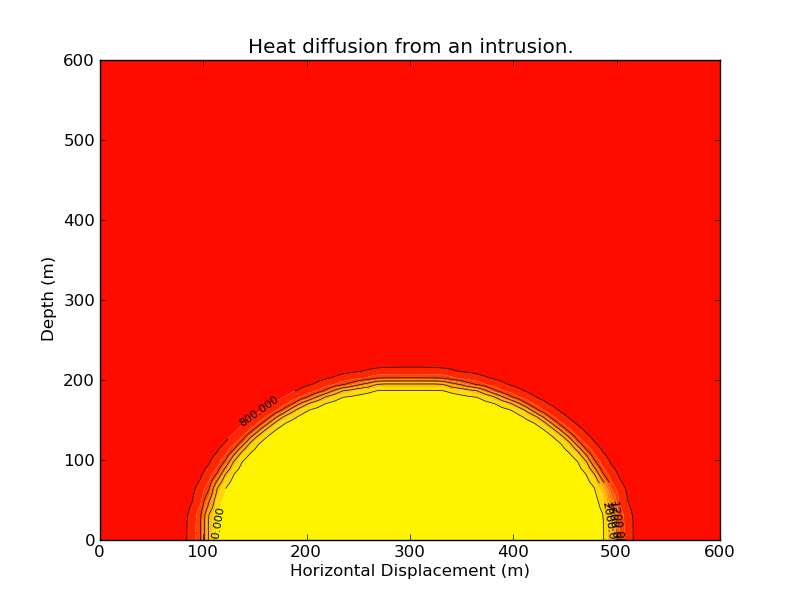
\includegraphics[width=4.in]{figures/heatrefraction001.png}}
\centerline{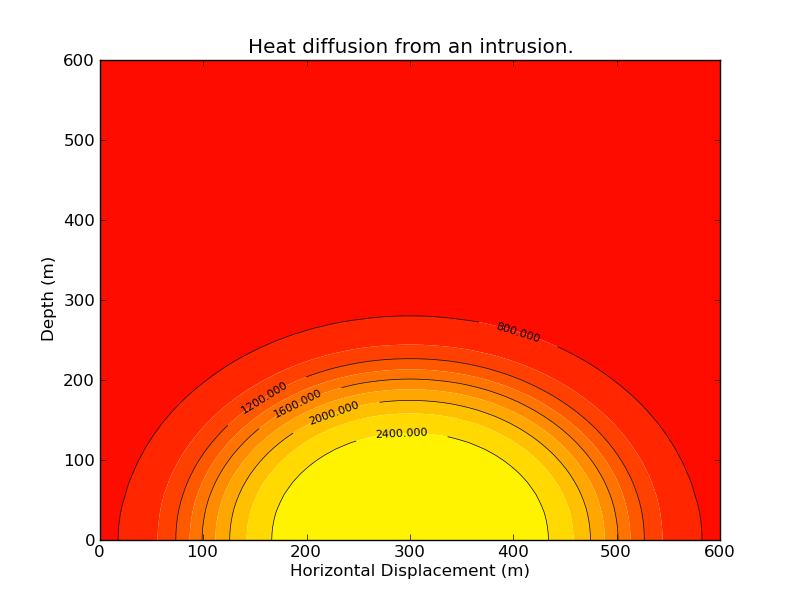
\includegraphics[width=4.in]{figures/heatrefraction030.png}}
\centerline{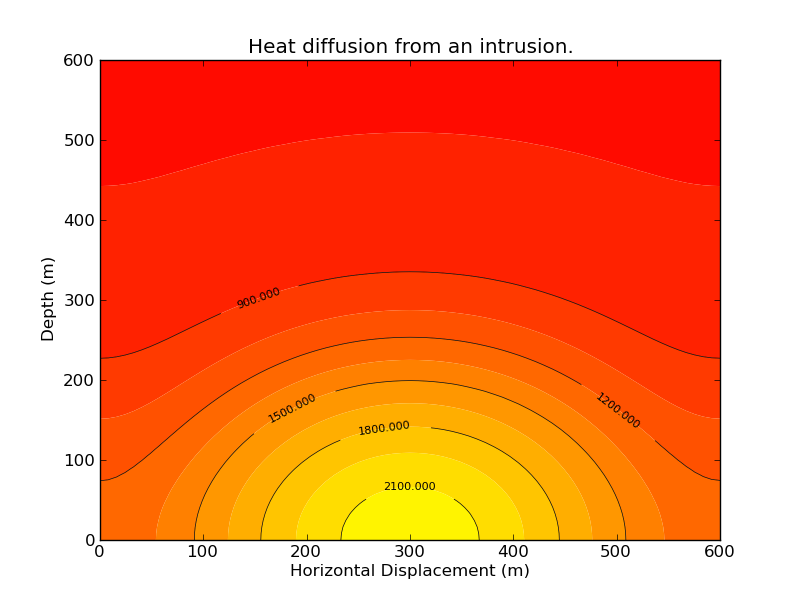
\includegraphics[width=4.in]{figures/heatrefraction200.png}}
\caption{Example 3a: 2D model: Total temperature distribution ($T$) at time step
$1$, $20$ and $200$. Contour lines show temperature.}
\label{fig:twodhdans}
\end{figure}

\section{Contouring \esc Data using \modmpl.}
\label{Sec:2DHD plot}
To complete our transition from a 1D to a 2D model we also need to modify the 
plotting procedure. As before we use \modmpl to do the plotting in this case a
contour plot. For 2D contour plots \modmpl expects that the data are regularly
gridded. We have no control over the location and ordering of the sample points
used to represent the solution. Therefore it is necessary to interpolate our
solution onto a regular grid.

In \refSec{sec: plot T} we have already learned how to extract the $x$
coordinates of sample points as 
\verb|numpy| array to hand the values to \modmpl. This can easily be extended
to extract both the $x$ and the $y$ coordinates;
\begin{python}
import numpy as np
def toXYTuple(coords):
    coords = np.array(coords.toListOfTuples()) #convert to Tuple
    coordX = coords[:,0] #X components.
    coordY = coords[:,1] #Y components.
    return coordX,coordY
\end{python}
For convenience we have put this function into \file{clib.py} so we can use
this function in other scripts more easily. 

We now generate a regular $100 \times 100$ grid over the domain ($mx$ and $my$ 
are the dimensions in the $x$ and $y$ directions) which is done using the
\modnumpy function \verb|linspace|.
\begin{python}
from clib import toXYTuple
# get sample points for temperature as  for contouring      
coordX, coordY = toXYTuple(T.getFunctionSpace().getX())
# create regular grid
xi = np.linspace(0.0,mx,75)
yi = np.linspace(0.0,my,75)
\end{python}
The values \verb|[xi[k], yi[l]]| are the grid points.

The remainder of our contouring commands resides within a \verb|while| loop so
that a new contour is generated for each time step. For each time step the
solution must be re-gridded for \modmpl using the \verb|griddata| function. This
function interprets irregularly located values \verb|tempT| at locations defined
by \verb|coordX| and \verb|coordY| as values at the new coordinates of a
rectangular grid defined by
\verb|xi| and \verb|yi|. The output is \verb|zi|. It is now possible to use the
\verb|contourf| function which generates colour filled contours. The colour
gradient of our plots is set via the command 
\verb|pl.matplotlib.pyplot.autumn()|, other colours are listed on the \modmpl web page\footnote{see
\url{http://matplotlib.sourceforge.net/api/}}. Our results are then contoured,
visually adjusted using the \modmpl functions and then saved to a file.
\verb|pl.clf()| clears the figure in readiness for the next time iteration.
\begin{python}
#grid the data.
zi = pl.matplotlib.mlab.griddata(coordX,coordY,tempT,xi,yi)
# contour the gridded data, plotting dots at the randomly spaced data points.
pl.matplotlib.pyplot.autumn()
pl.contourf(xi,yi,zi,10)
CS = pl.contour(xi,yi,zi,5,linewidths=0.5,colors='k')
pl.clabel(CS, inline=1, fontsize=8)
pl.axis([0,600,0,600])
pl.title("Heat diffusion from an intrusion.")
pl.xlabel("Horizontal Displacement (m)")
pl.ylabel("Depth (m)")
pl.savefig(os.path.join(save_path,"Tcontour%03d.png") %i)
pl.clf()        
\end{python}
The function \verb|pl.contour| is used to add labelled contour lines to the
plot. 
The results for selected time steps are shown in \reffig{fig:twodhdans}.


\section{Advanced Visualisation using VTK}

\sslist{example03b.py}
An alternative approach to \modmpl for visualisation is the usage of a package
which is based on the Visualization Toolkit (VTK) library\footnote{see \url{http://www.vtk.org/}}.
There is a variety of packages available. Here we use the package \mayavi\footnote{see
\url{http://code.enthought.com/projects/mayavi/}} as an example. 

\mayavi is an interactive, GUI driven tool which is 
really designed to visualise large three dimensional data sets where \modmpl 
is not suitable. But it is also very useful when it comes to two dimensional
problems. 
The decision of which tool is the best can be subjective and users should
determine which package they require and are most comfortable with. The main
difference between using \mayavi (or other VTK based tools) and \modmpl is that
the actual visualisation is detached from the calculation by writing the
results to external files and importing them into \mayavi. In 3D the best
camera position for rendering a scene is not obvious before the results are
available. Therefore the user may need to try different settings before the
best is found. Moreover, in many cases a 3D interactive visualisation is the
only way to really understand the results (e.g. using stereographic projection).

To write the temperatures at each time step to data files in the VTK file format
one needs to import \verb|saveVTK| from the \weipa module and call it:
\begin{python}
from esys.weipa import saveVTK
while t<=tend:
      i+=1 #counter
      t+=h #current time
      mypde.setValue(Y=qH+T*rhocp/h)
      T=mypde.getSolution()
      saveVTK(os.path.join(save_path,"data.%03d.vtu"%i, T=T)
\end{python}
The data files, e.g. \file{data.001.vtu}, contain all necessary information to 
visualise the temperature and can be directly processed by \mayavi. Note that
there is no re-gridding required. The file extension \file{.vtu} is
automatically added if not supplied to \verb|saveVTK|. 

\begin{figure}[ht]
\centerline{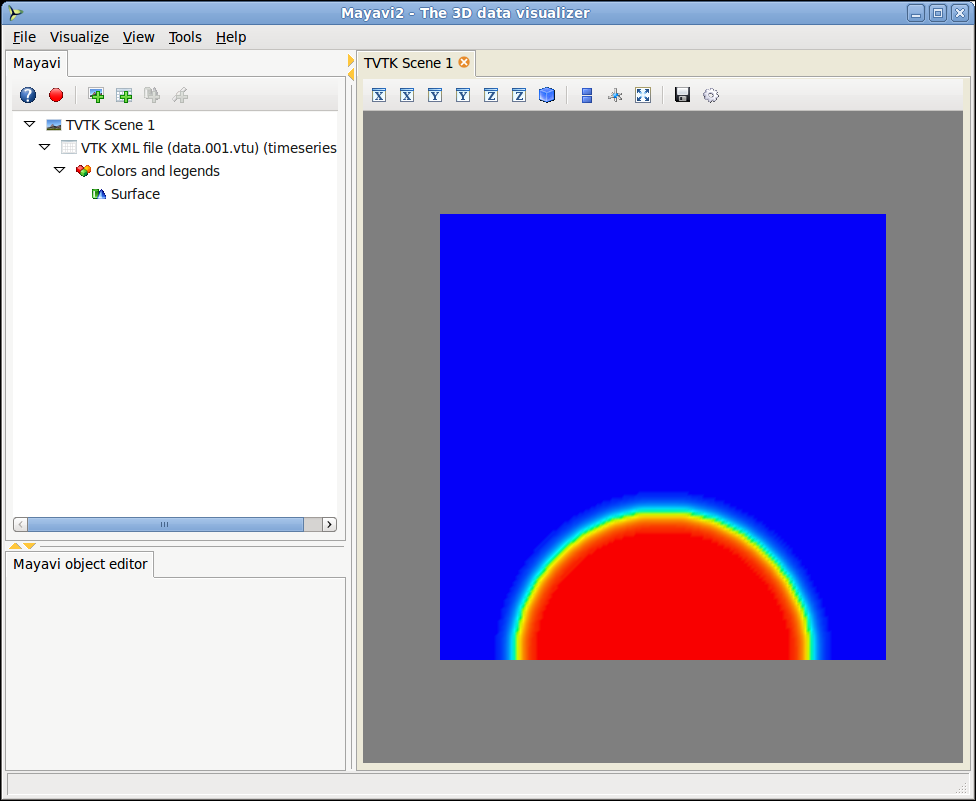
\includegraphics[width=4.in]{figures/ScreeshotMayavi2n1}}
\caption{Example 3b: \mayavi start up window}
\label{fig:mayavi window}
\end{figure}

\begin{figure}[ht]
\centerline{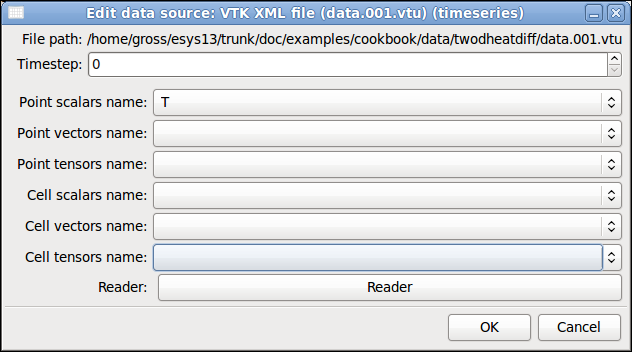
\includegraphics[width=4.in]{figures/ScreeshotMayavi2n2}}
\caption{Example 3b: \mayavi data control window}
\label{fig:mayavi window2}
\end{figure}
After you run the script you will find the 
result files \file{data.*.vtu} in the result directory \file{data/example03}.
Run the command
\begin{python}
>> mayavi2 -d data.001.vtu -m Surface &
\end{python}
from the result directory. \mayavi will start up a window similar to
\reffig{fig:mayavi window}.
The right hand side shows the temperature at the first time step. To show
the results at other time steps you can click at the item \texttt{VTK XML file
(data.001.vtu) (timeseries)}
at the top left hand side. This will bring up a new window similar to the window
shown in \reffig{fig:mayavi window2}. By clicking at the arrows in the top
right corner you can move forwards and backwards in time. 
You will also notice the text \textbf{T} next to the item \texttt{Point scalars
name}. The
name \textbf{T} corresponds to the keyword argument name \texttt{T} we have
used in the \verb|saveVTK| call. In this menu item you can select other results
you may have written to the output file for visualisation.

\textbf{For the advanced user}: Using the \modmpl to visualise spatially
distributed data is not MPI compatible. However, the \verb|saveVTK| function
can be used with MPI. In fact, the function collects the values of the sample
points spread across processor ranks into a single file.
For more details on writing scripts for parallel computing please consult the
\emph{user's guide}.


% % % % 
\chapter{Complex Geometries}
 \label{CHAP HEAT 2}
 
%%%%%%%%%%%%%%%%%%%%%%%%%%%%%%%%%%%%%%%%%%%%%%%%%%%%%%%%
%
% Copyright (c) 2003-2012 by University of Queensland
% Earth Systems Science Computational Center (ESSCC)
% http://www.uq.edu.au/esscc
%
% Primary Business: Queensland, Australia
% Licensed under the Open Software License version 3.0
% http://www.opensource.org/licenses/osl-3.0.php
%
%%%%%%%%%%%%%%%%%%%%%%%%%%%%%%%%%%%%%%%%%%%%%%%%%%%%%%%%

\section{Steady-state Heat Refraction}
\label{STEADY-STATE HEAT REFRACTION}

In this chapter we demonstrate how to handle more complex geometries. 

Steady-state heat refraction will give us an opportunity to investigate some of
the richer features that the \esc package has to offer. One of these is \pycad .
The advantage of using \pycad is that it offers an easy method for developing
and manipulating complex domains. In conjunction with \gmsh we can generate
finite element meshes that conform to our domain's shape providing accurate
modelling of interfaces and boundaries. Another useful function of \pycad is
that we can tag specific areas of our domain with labels as we construct them.
These labels can then be used in \esc to define properties like material
constants and source locations. 

We proceed in this chapter by first looking at a very simple geometry. Whilst a
simple rectangular domain is not very interesting the example is elaborated upon
later by introducing an internal curved interface.

\section{Example 4: Creating the Domain with \pycad}
\label{example4}
\sslist{example04a.py}
We modify the example in Chapter~\ref{CHAP HEAT 2a} in two ways: we look at the
steady state case with slightly modified boundary conditions and use a more
flexible tool to generate the geometry. Let us look at the geometry first. 

We want to define a rectangular domain of width $5 km$ and depth $6 km$ below
the surface of the Earth. The domain is subject to a few conditions. The
temperature is known at the surface and the basement has a known heat flux. Each
side of the domain is insulated and the aim is to calculate the final
temperature distribution.

In \pycad there are a few primary constructors that build upon each other to
define domains and boundaries. The ones we use are:
\begin{python}
from esys.pycad import *
Point() #Create a point in space.
Line() #Creates a line from a number of points.
CurveLoop() #Creates a closed loop from a number of lines.
PlaneSurface() #Creates a surface based on a CurveLoop
\end{python}
So to construct our domain as shown in \reffig{fig:pycad rec}, we first need to
create the corner points. From the corner points we build the four edges of the
rectangle. The four edges then form a closed loop which defines our domain as a
surface. We start by inputting the variables we need to construct the model.
\begin{python}
width=5000.0*m   #width of model
depth=-6000.0*m  #depth of model
\end{python} 

\begin{figure}[ht]
\centerline{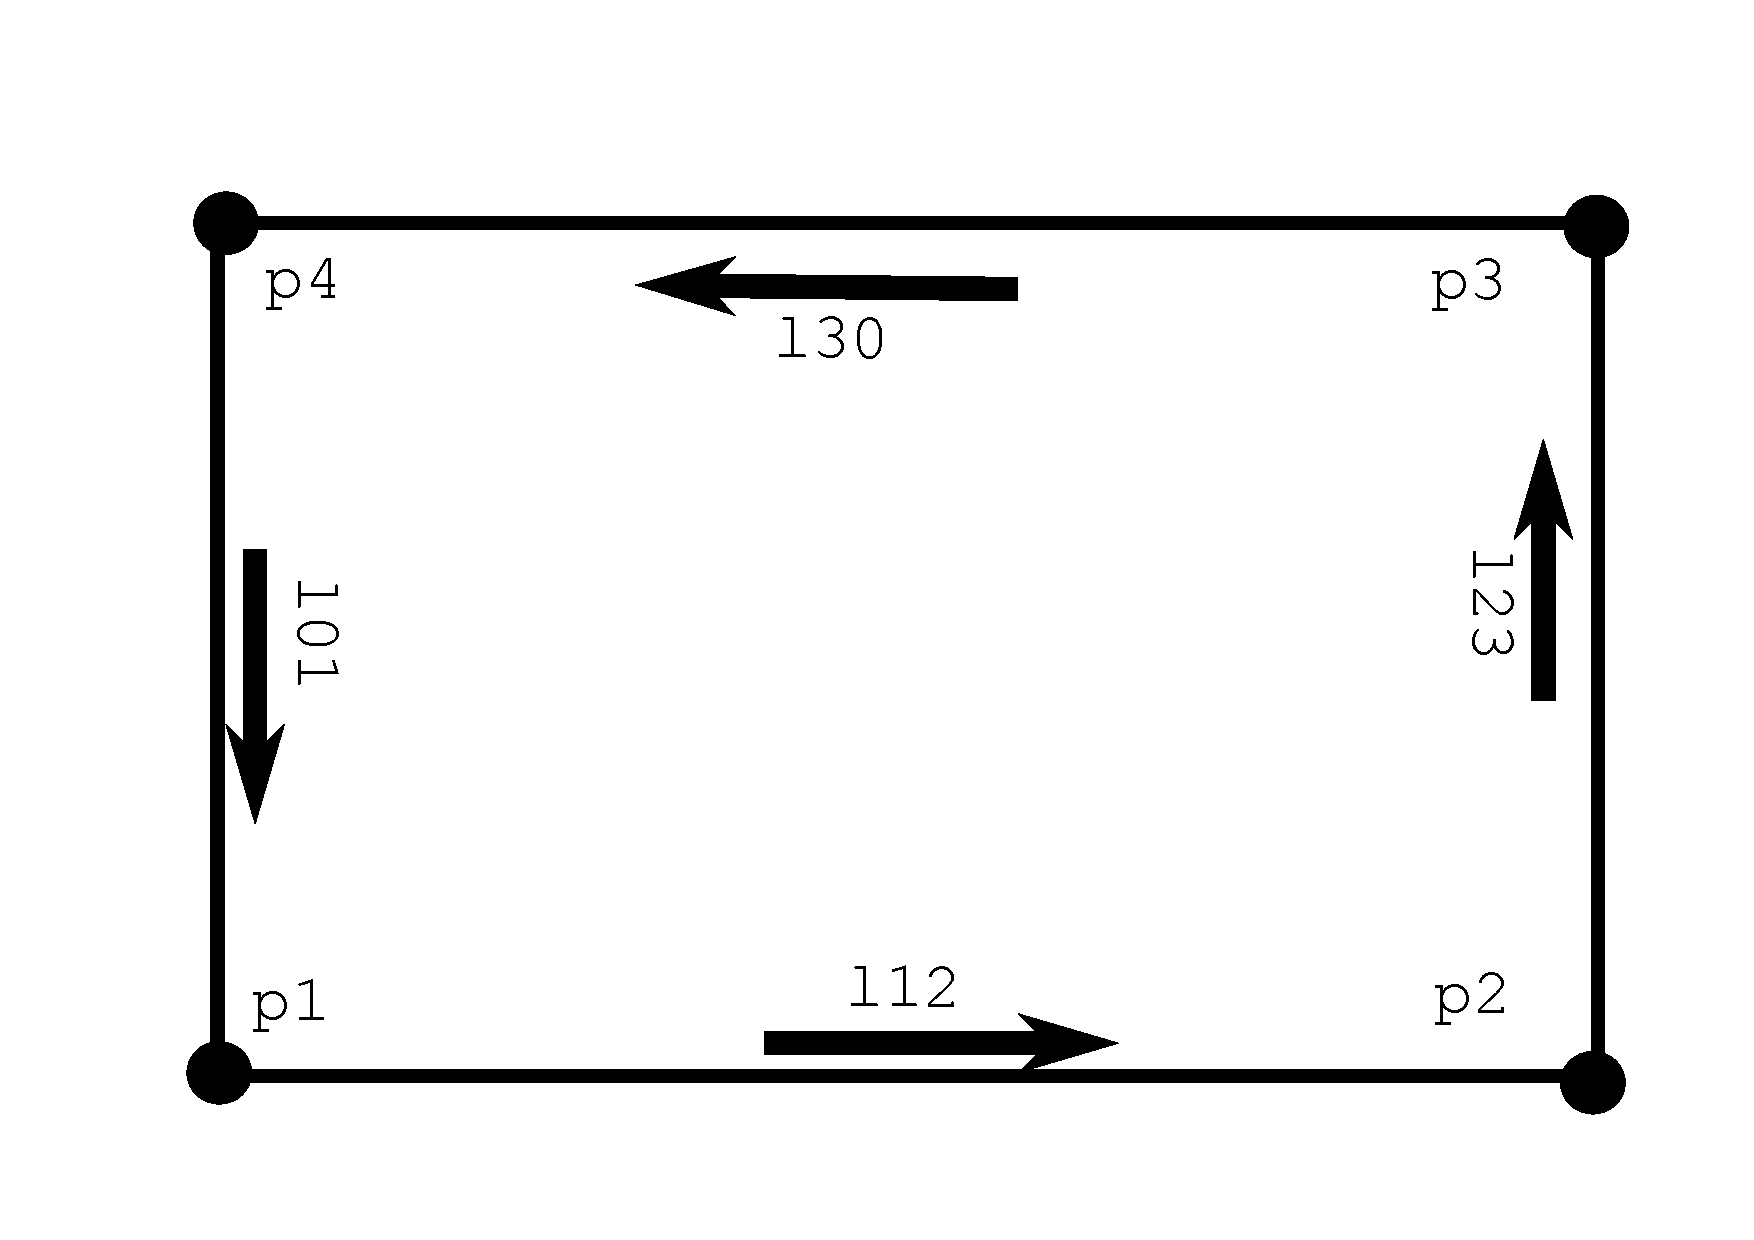
\includegraphics[width=4.in]{figures/pycadrec}}
\caption{Example 4: Rectangular Domain for \pycad}
\label{fig:pycad rec}
\end{figure}

The variables are then used to construct the four corners of our domain, which
from the origin has the dimensions of $5000$ meters width and $-6000$ meters
depth. This is done with the \verb|Point()| function which accepts x, y and z
coordinates. Our domain is in two dimensions so z should always be zero.
\begin{python}
# Overall Domain
p0=Point(0.0,      0.0, 0.0)
p1=Point(0.0,    depth, 0.0)
p2=Point(width, depth, 0.0)
p3=Point(width,   0.0, 0.0)
\end{python}
Now lines are defined using our points. This forms a rectangle around our
domain:
\begin{python}
l01=Line(p0, p1)
l12=Line(p1, p2)
l23=Line(p2, p3)
l30=Line(p3, p0)
\end{python}
Note that lines have a direction. These lines form the basis for our domain
boundary, which is a closed loop.
\begin{python}
c=CurveLoop(l01, l12, l23, l30)
\end{python}
Be careful to define the curved loop in an \textbf{anti-clockwise} manner
otherwise the meshing algorithm may fail.
Finally we can define the domain as
\begin{python}
rec = PlaneSurface(c)
\end{python}
At this point the introduction of the curved loop seems to be unnecessary but
this concept plays an important role if holes are introduced. 

Now we are ready to hand over the domain \verb|rec| to a mesher which
subdivides the domain into triangles (or tetrahedra in 3D). In our case we use
\gmsh. We create an instance of the \verb|Design| class which will handle the
interface to \gmsh: 
\begin{python}
from esys.pycad.gmsh import Design 
d=Design(dim=2, element_size=200*m)
\end{python}
The argument \verb|dim| defines the spatial dimension of the domain\footnote{If
\texttt{dim}=3 the rectangle would be interpreted as a surface in the three
dimensional space.}. The second argument \verb|element_size| defines the element
size which is the maximum length of a triangle edge in the mesh. The element
size needs to be chosen with care in order to avoid very dense meshes. If the
mesh is too dense, the computational time will be long but if the mesh is too
sparse, the modelled result will be poor. In our case with an element size of
$200$m and a domain length of $6000$m we will end up with about $\frac{6000m}{200m}=30$
triangles in each spatial direction. So we end up with about $30 \times 30 =
900$ triangles which is a size that can be handled easily.
The domain \verb|rec| can simply be added to the \verb|Design|;
\begin{python}
d.addItem(rec)
\end{python}
We have the plan to set a heat flux on the bottom of the domain. One can use
the masking technique to do this but \pycad offers a more convenient technique
called tagging. With this technique items in the domain are named using the
\verb|PropertySet| class. We can then later use this name to set values
specifically for those sample points located on the named items. Here we name
the bottom face of the domain where we will set the heat influx
\footnote{In some applications, eg.
when dealing with influxes,
it is required to have the surface beeing meshed without the need of explicitly
name the surface. In this case the line forming the surface of the domain need to be
added to the \texttt{Design} 
using \texttt{d.addItem(rec, l01, l12, l23, l30)}}:
\begin{python}
ps=PropertySet("linebottom",l12))
d.addItem(ps)
\end{python}
Now we are ready to hand over the \verb|Design| to \FINLEY:
\begin{python}
from esys.finley import MakeDomain
domain=MakeDomain(d)
\end{python}
The \verb|domain| object can now be used in the same way like the return object
of the \verb|Rectangle| object we have used previously to generate a mesh. It
is common practice to separate the mesh generation from the PDE solution.
The main reason for this is that mesh generation can be computationally very
expensive in particular in 3D. So it is more efficient to generate the mesh
once and write it to a file. The mesh can then be read in every time a new
simulation is run. \FINLEY supports this in the following 
way\footnote{An alternative is using the \texttt{dump} and \texttt{load}
functions. They work with a binary format and tend to be much smaller.}:
\begin{python}
# write domain to a text file
domain.write("example04.fly")
\end{python}
and then for reading in another script:
\begin{python}
# read domain from text file
from esys.finley import ReadMesh
domain =ReadMesh("example04.fly")
\end{python}

Before we discuss how to solve the PDE for this problem, it is useful to
present two additional options of the \verb|Design| class. 
These allow the user to access the script which is used by \gmsh to generate
the mesh as well as the generated mesh itself. This is done by setting specific
names for these files: 
\begin{python}
d.setScriptFileName("example04.geo")
d.setMeshFileName("example04.msh")
\end{python}
Conventionally the extension \texttt{geo} is used for the script file of the
\gmsh geometry and the extension \texttt{msh} for the mesh file. Normally these
files are deleted after usage.
Accessing these files can be helpful to debug the generation of more complex
geometries. The geometry and the mesh can be visualised from the command line
using
\begin{verbatim}
gmsh example04.geo  # show geometry
gmsh example04.msh  # show mesh
\end{verbatim}
The mesh is shown in \reffig{fig:pycad rec mesh}.

\begin{figure}[ht]
\centerline{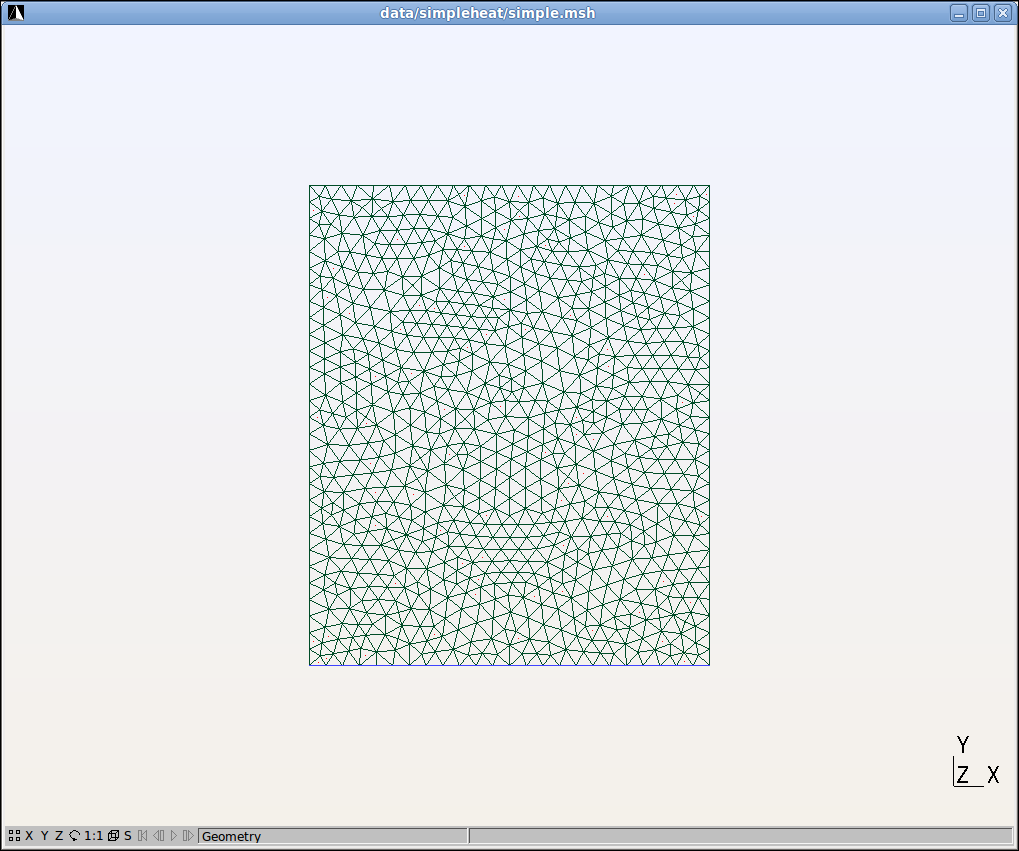
\includegraphics[width=4.in]{figures/simplemesh}}
\caption{Example 4a: Mesh over rectangular domain, see \reffig{fig:pycad rec}}
\label{fig:pycad rec mesh}
\end{figure}
\clearpage

\section{The Steady-state Heat Equation}
\sslist{example04b.py, cblib}
A temperature equilibrium or steady state is reached when the temperature
distribution in the model does not change with time. To calculate the steady
state solution the time derivative term in \refEq{eqn:Tform nabla} needs to be
set to zero;
\begin{equation}\label{eqn:Tform nabla steady}
-\nabla \cdot \kappa \nabla T = q_H
\end{equation}
This PDE is easier to solve than the PDE in \refEq{eqn:hdgenf2}, as no time
steps (iterations) are required. The \verb|D| term from \refEq{eqn:hdgenf2} is
simply dropped in this case.
\begin{python}
mypde=LinearPDE(domain)
mypde.setValue(A=kappa*kronecker(model), Y=qH)
\end{python}
The temperature at the top face of the domain is known as \verb|Ttop|~($=20 C$).
In \refSec{Sec:1DHDv0} we have already discussed how this constraint is added
to the PDE:
\begin{python}
x=Solution(domain).getX()
mypde.setValue(q=whereZero(x[1]-sup(x[1])),r=Ttop)
\end{python}
Notice that we use the \verb|sup| function to calculate the maximum of $y$
coordinates of the relevant sample points.

In all cases so far we have assumed that the domain is insulated which
translates into a zero normal flux $-n \cdot \kappa \nabla T$, see
\refEq{eq:hom flux}. In the modelling set-up of this chapter we want to set
the normal heat flux at the bottom to \verb|qin| while still maintaining
insulation at the left and right face. Mathematically we can express this as
\begin{equation}
-n \cdot \kappa \nabla T = q_{S}
\label{eq:inhom flux}
\end{equation}
where $q_{S}$ is a function of its location on the boundary. Its value
becomes zero for locations on the left or right face of the domain while it has
the value \verb|qin| at the bottom face.
Notice that the value of $q_{S}$ at the top face is not relevant as we
prescribe the temperature here.
We could define $q_{S}$ by using the masking techniques demonstrated
earlier. The tagging mechanism provides an alternative and in many cases more
convenient way of defining piecewise constant functions such as
$q_{S}$. Recall now that the bottom face was denoted with the name
\verb|linebottom| when we defined the domain.
We can use this now to create $q_{S}$;
\begin{python}
qS=Scalar(0,FunctionOnBoundary(domain))
qS.setTaggedValue("linebottom",qin)
\end{python}
In the first line \verb|qS| is defined as a scalar value over the sample points
on the boundary of the domain. It is initialised to zero for all sample points.
In the second statement the values for those sample points which are located on
the line marked by \verb|linebottom| are set to \verb|qin|. 

The Neumann boundary condition assumed by \esc has the form
\begin{equation}\label{NEUMAN 2b}
n\cdot A \cdot\nabla u = y 
\end{equation}
In comparison to the version in \refEq{NEUMAN 2} we have used so far the right
hand side is now the new PDE coefficient $y$. As we have not specified $y$ in
our previous examples, \esc has assumed the value zero for $y$. A comparison of
\refEq{NEUMAN 2b} and \refEq{eq:inhom flux} reveals that one needs to choose
$y=-q_{S}$;
\begin{python}
qS=Scalar(0,FunctionOnBoundary(domain))
qS.setTaggedValue("linebottom",qin)
mypde.setValue(y=-qS)
\end{python}
To plot the results we use the \modmpl library as shown in
\refSec{Sec:2DHD plot}. For convenience the interpolation of the temperature to
a rectangular grid for contour plotting is made available via the
\verb|toRegGrid| function in the \verb|cblib| module. Your result should look
similar to \reffig{fig:steady state heat}.

\begin{figure}[ht]
\centerline{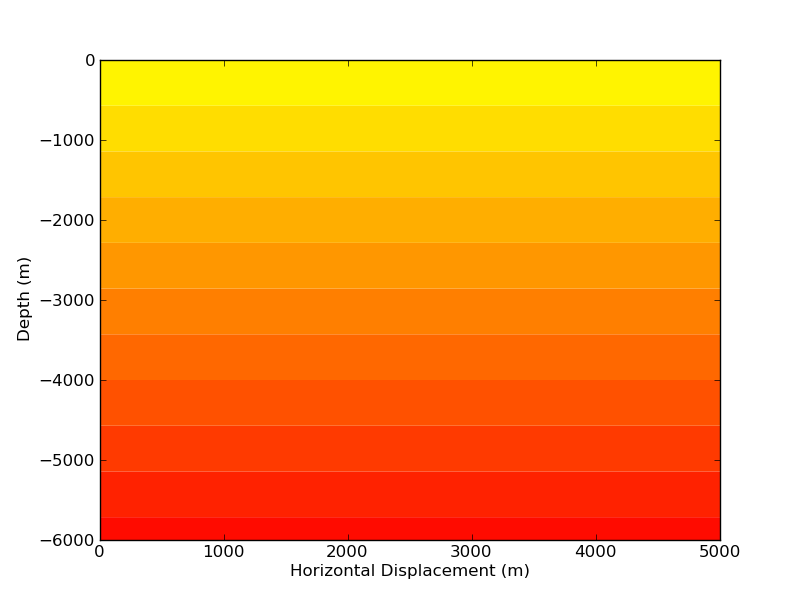
\includegraphics[width=4.in]{figures/simpleheat}}
\caption{Example 4b: Result of simple steady state heat problem}
\label{fig:steady state heat}
\end{figure}
\clearpage


 
%%%%%%%%%%%%%%%%%%%%%%%%%%%%%%%%%%%%%%%%%%%%%%%%%%%%%%%%%%%%%%%%%%%%%%%%%%%%%%
% Copyright (c) 2003-2015 by University of Queensland
% http://www.uq.edu.au
%
% Primary Business: Queensland, Australia
% Licensed under the Open Software License version 3.0
% http://www.opensource.org/licenses/osl-3.0.php
%
% Development until 2012 by Earth Systems Science Computational Center (ESSCC)
% Development 2012-2013 by School of Earth Sciences
% Development from 2014 by Centre for Geoscience Computing (GeoComp)
%
%%%%%%%%%%%%%%%%%%%%%%%%%%%%%%%%%%%%%%%%%%%%%%%%%%%%%%%%%%%%%%%%%%%%%%%%%%%%%%

\section{Example 5: A Heat Refraction Model}
\label{example5}
\sslist{example05a.py and cblib.py}
Our heat refraction model will be a large anticlinal structure that is subject
to a constant temperature at the surface and experiencing a steady heat flux at
its base. Our aim is to show that the temperature flux across the surface is
not linear from bottom to top, but is in fact warped by the structure of the
model. The heat flow pattern demonstrates the dependence upon the material
properties and the shape of the interface.

The script of \refSec{example4} is modified by subdividing the block into two
parts. The curve separating the two blocks is given as a spline, see
\reffig{fig:anticlinehrmodel}. The data points
used to define the curve may be imported from a database of measurements
(\textit{e.g.} borehole depth data), but for simplicity it is assumed here that
the coordinates are known in an analytic form.

\begin{figure}[ht]
\centerline{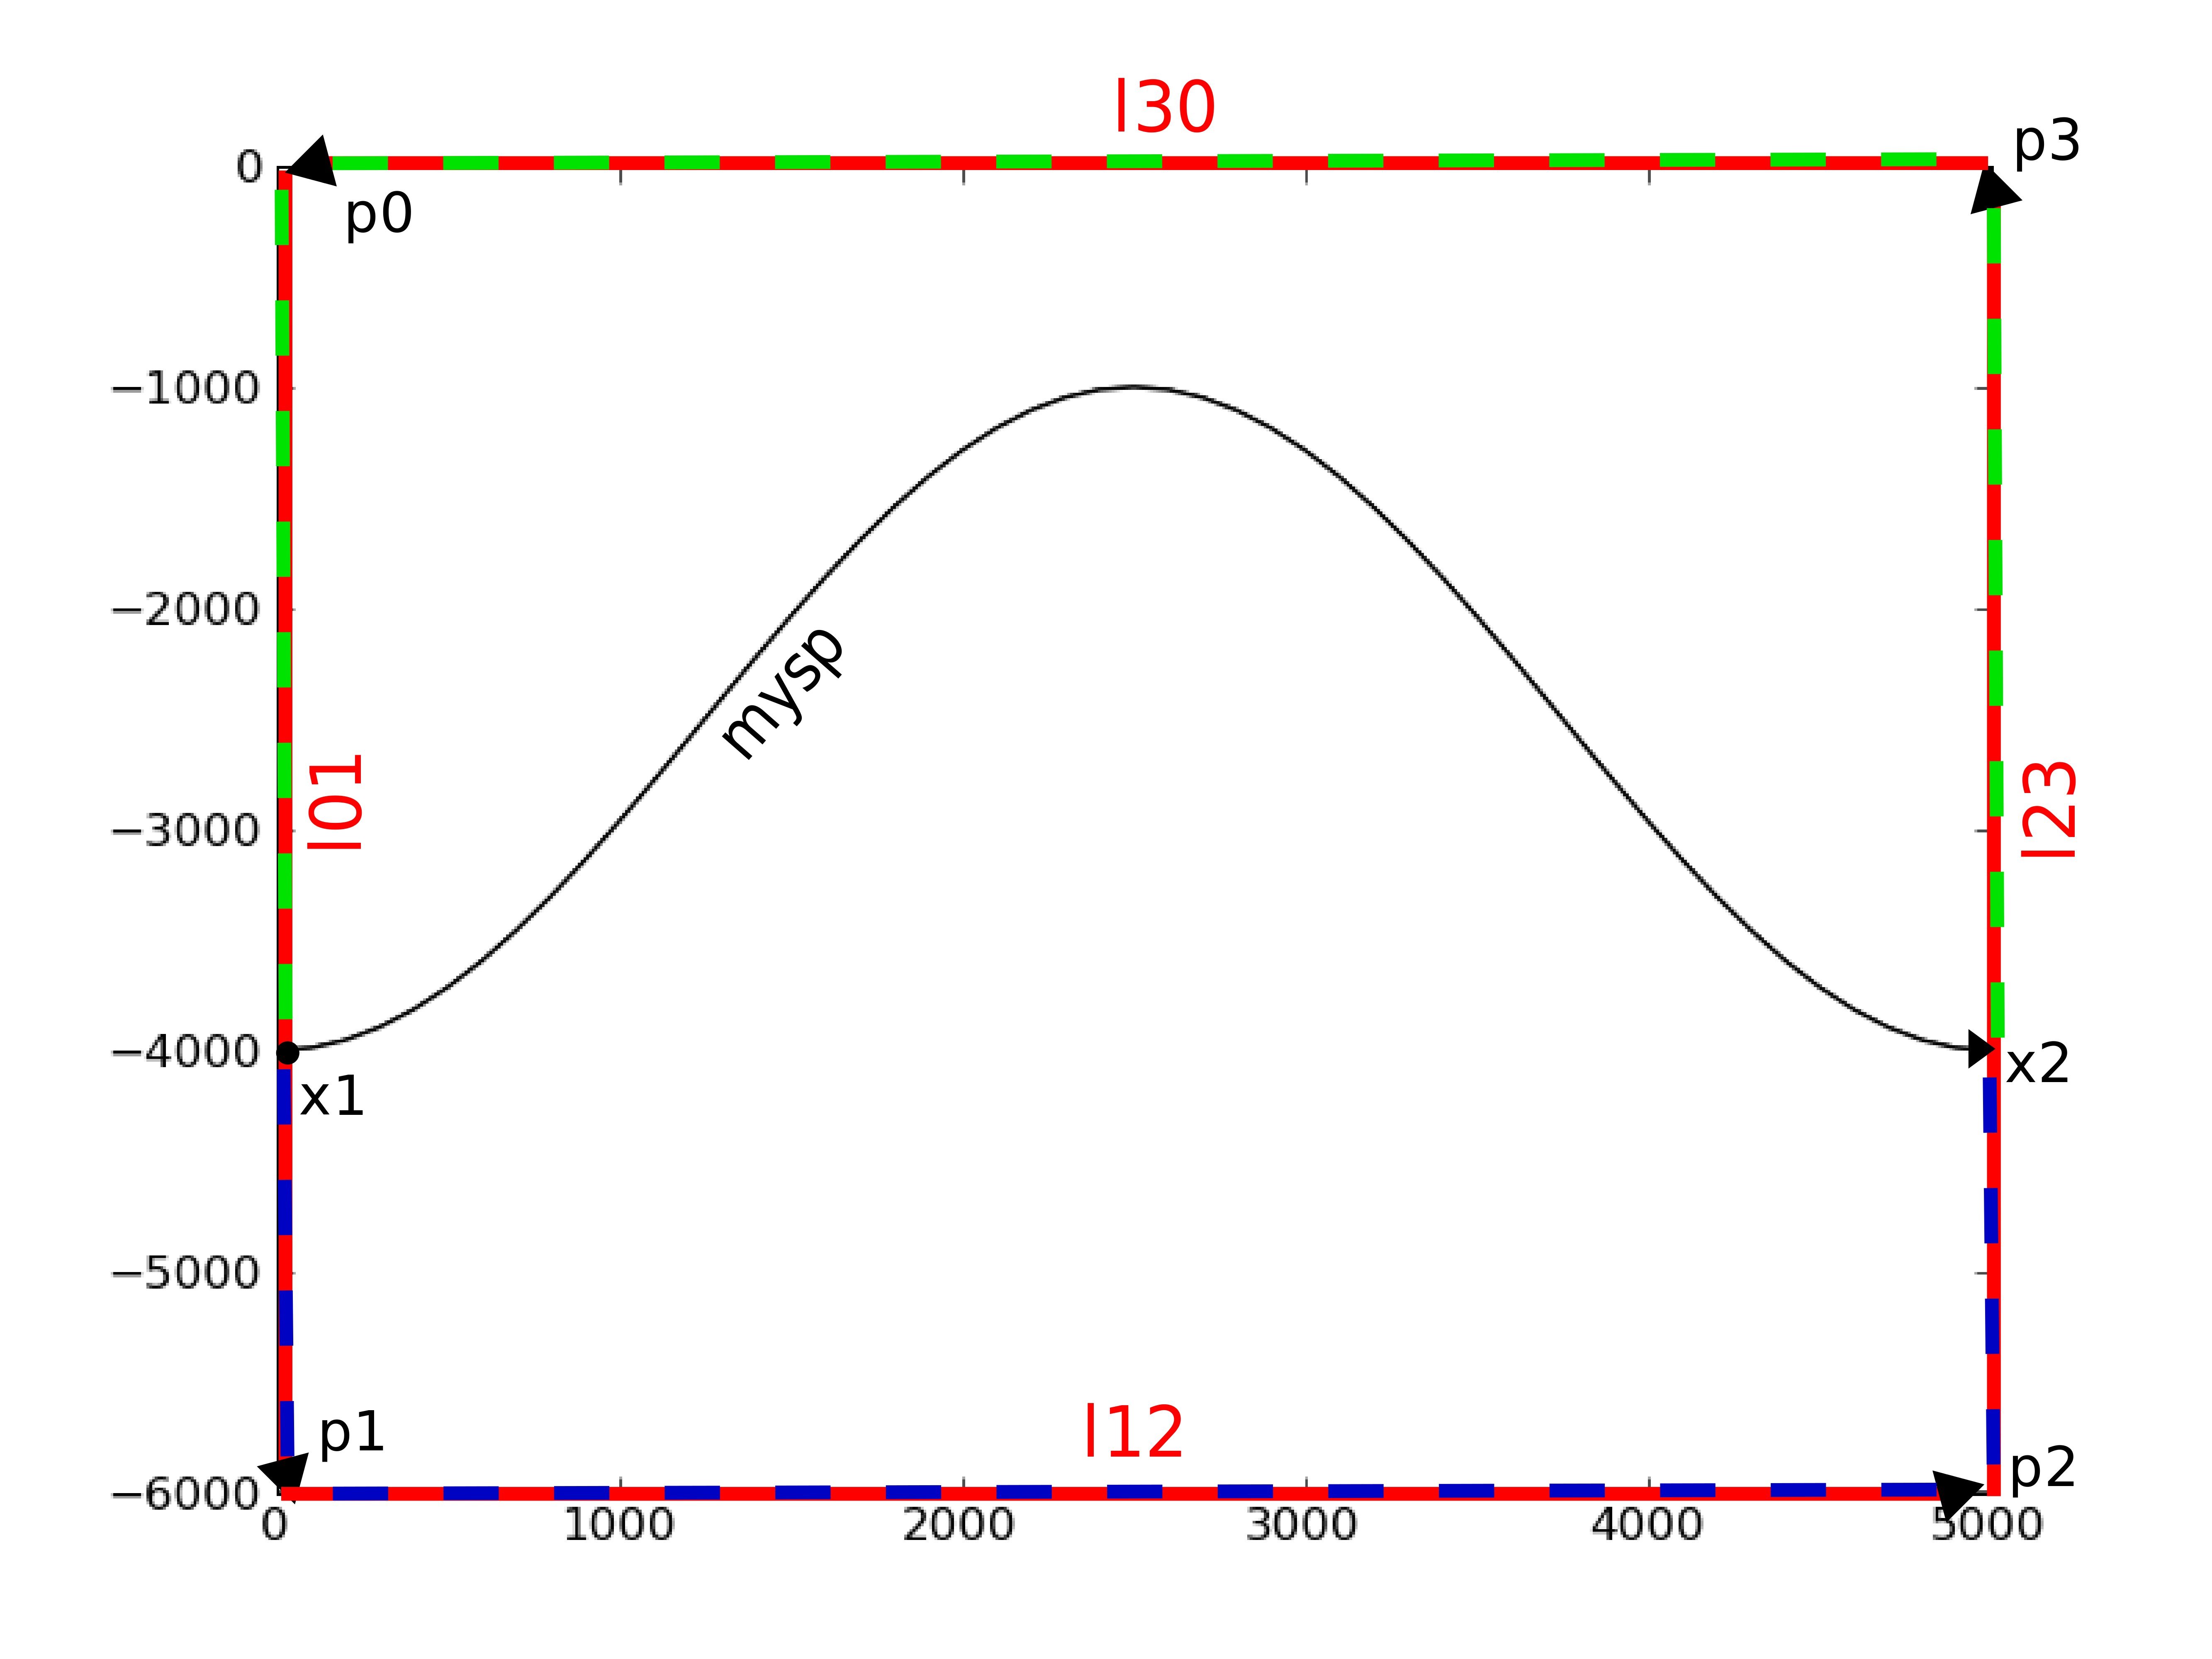
\includegraphics[width=4.in]{figures/anticlineheatrefraction.png}}
\caption{Example 5a: Heat refraction model with point and line labels}
\label{fig:anticlinehrmodel}
\end{figure}

There are two modes available in this example. When \verb|modal=1|, this
indicates to the script that the model should be an anticline. Otherwise, when
\verb|modal=-1|, the model is a syncline. The modal operator simply changes the
orientation of the boundary function so that it is either upwards or downwards
curving. A \verb|save_path| has also been defined so that we can easily separate
our data from other examples and our scripts. 

It is now possible to start defining our domain and boundaries. 

The curve defining our clinal structure is located approximately in the middle
of the domain and has a sinusoidal shape. We define the curve by generating
points at discrete intervals; $51$ in this case, and then create a smooth curve
through the points using the \verb|Spline()| function.
\begin{python}
# Material Boundary
x=[ Point(i*dsp\
    ,-dep_sp+modal*orit*h_sp*cos(pi*i*dsp/dep_sp+pi))\
     for i in range(0,sspl)\
    ]
mysp = Spline(*tuple(x)) #*tuple() forces x to become a tuple
\end{python}
The start and end points of the spline can be returned to help define the
material boundaries.
\begin{python}
x1=mysp.getStartPoint()
x2=mysp.getEndPoint()
\end{python}
The top block or material above the clinal/spline boundary is defined in an
\textbf{anti-clockwise} manner by creating lines and then a closed loop. By
meshing the sub-domain we also need to assign it a planar surface. 
\begin{python}
# TOP BLOCK
tbl1=Line(p0,x1)
tbl2=mysp
tbl3=Line(x2,p3)
l30=Line(p3, p0)
tblockloop = CurveLoop(tbl1,tbl2,tbl3,l30)
tblock = PlaneSurface(tblockloop)
\end{python}
This process is repeated for every other sub-domain. In this example there is
only one other, the bottom block. The process is similar to the top block but
with a few differences. The spline points must be reversed by setting the spline
as negative.
\begin{python}
bbl4=-mysp
\end{python}
This reverse spline option unfortunately does not work for the
\verb|getLoopCoords| command, however, the \modmpl polygon tool will accept
clock-wise oriented points so we can define a new curve.
\begin{python}
#clockwise check
bblockloop=CurveLoop(mysp,Line(x2,p2),Line(p2,p1),Line(p1,x1))
\end{python}
The last few steps in creating the domain require that the previously defined
domain and sub-domain points are submitted to generate a mesh that can be
imported into \esc.
To initialise the mesh it first needs some design parameters. In this case we
have 2 dimensions \verb|dim| and a specified number of finite elements that need
to be applied to the domain \verb|element_size|. It then becomes a simple task
of adding the sub-domains and flux boundaries to the design. Each element of our
model can be given an identifier which makes it easier to define the sub-domain
properties in the solution script. This is done using the 
\verb|PropertySet()| function. The geometry and mesh are then saved so the
\esc domain can be created.
\begin{python}
# Create a Design which can make the mesh
d=Design(dim=2, element_size=200)
# Add the sub-domains and flux boundaries.
d.addItems(PropertySet("top",tblock),PropertySet("bottom",bblock),\
                   PropertySet("linebottom",l12))
# Create the geometry, mesh and escript domain
d.setScriptFileName(os.path.join(save_path,"example05.geo"))
d.setMeshFileName(os.path.join(save_path,"example05.msh"))
domain=MakeDomain(d,optimizeLabeling=True)
\end{python}
The creation of our domain and its mesh is now complete.

With the mesh imported it is now possible to use our tagging property to set up
our PDE coefficients. In this case $\kappa$ is set via the
\verb|setTaggedValue()| function which takes two arguments, the name of the
tagged points and the value to assign to them. 
\begin{python}
# set up kappa (thermal conductivity across domain) using tags
kappa=Scalar(0,Function(domain))
kappa.setTaggedValue("top",2.0*W/m/K)
kappa.setTaggedValue("bottom",4.0*W/m/K)
\end{python}
No further changes are required to the PDE solution step, see
\reffig{fig:anticlinetemp} for the result. 

\begin{figure}[ht]
\centerline{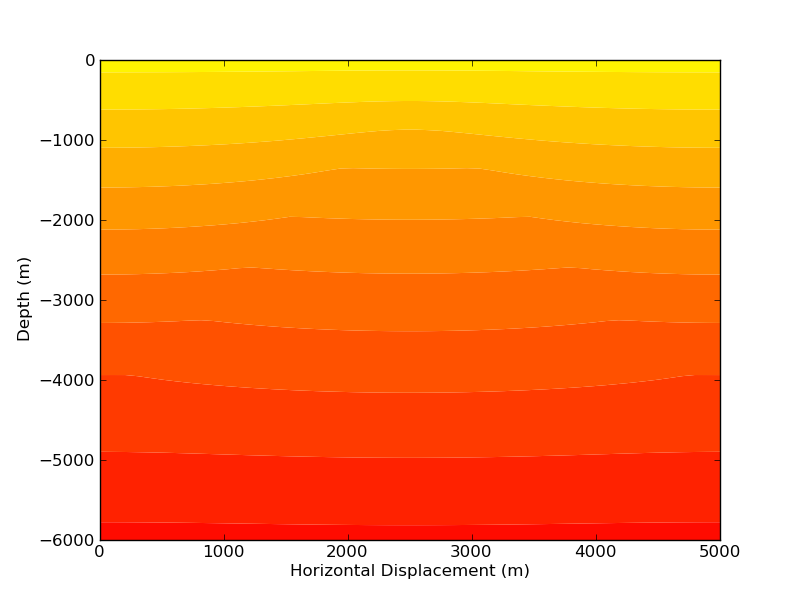
\includegraphics[width=4.in]{figures/heatrefraction}}
\caption{Example 5a: Temperature Distribution in the Heat Refraction Model}
\label{fig:anticlinetemp}
\end{figure}
\clearpage

\section{Line Profiles of 2D Data}
\sslist{example05b.py and cblib.py}
We want to investigate the profile of the data of the last example. 
Of particular interest is the depth profile of the heat flux which is the
second component of $-\kappa \nabla T$. The script from the previous section
is extended to show how a vertical profile can be plotted.

The first important piece of information, is that \esc assumes that $-\kappa
\nabla T$ is not smooth and that the point values of this solution are defined
at numerical interpolation points. This assumption is reasonable as
the flux is the product of the piecewise constant function $\kappa$ and 
the gradient of the temperature $T$ which has a discontinuity at the rock
interface.
Before plotting this function we need to smooth the solution using the
\verb|Projector()| class;
\begin{python}
from esys.escript.pdetools import Projector
proj=Projector(domain)
qu=proj(-kappa*grad(T))
\end{python}
The \verb|proj| object provides a mechanism to distribute values given at the
numerical interpolation points to the nodes of the FEM mesh - the heat flux in
this example. \verb|qu| has the same function space as the temperature
\verb|T|. The smoothed flux is interpolated to a regular $200\times 200$ grid
via;
\begin{python}
xiq,yiq,ziq = toRegGrid(qu[1],200,200)
\end{python}
using the \verb|toRegGrid| function from the cookbook library which we are
using for the contour plot.
At return \verb|ziq[j,i]| is the value of vertical heat flux at point
(\verb|xiq[i]|,\verb|yiq[j]|). We can easily create deep profiles now by
plotting slices \verb|ziq[:,i]| over \verb|yiq|. The following script
creates a deep profile at $x_{0}=\frac{width}{2}$;
\begin{python}
cut=int(len(xiq)/2)
pl.plot(ziq[:,cut]*1000.,yiq)
pl.title("Vertical Heat Flow Depth Profile")
pl.xlabel("Heat Flow (mW/m^2)")
pl.ylabel("Depth (m)")
pl.savefig(os.path.join(save_path,"hf.png"))
\end{python}
This process can be repeated for various variations of the solution.
\reffig{figs:dps} shows temperature, temperature gradient, thermal conductivity
and heat flow.

\begin{figure}[htp]
\centering
    \subfigure[Temperature Depth
Profile]{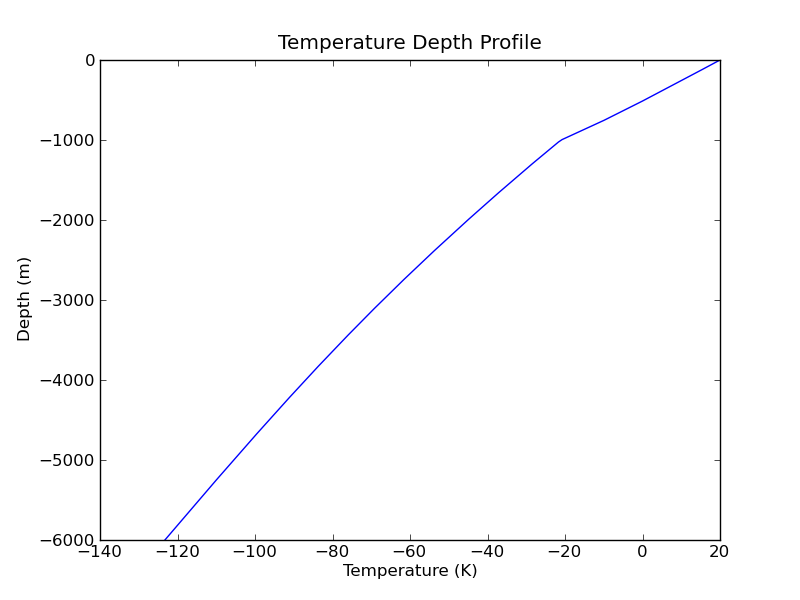
\includegraphics[width=3in]{figures/heatrefractiontdp.png}\label{
fig:tdp}}
    \subfigure[Temperature Gradient Depth
Profile]{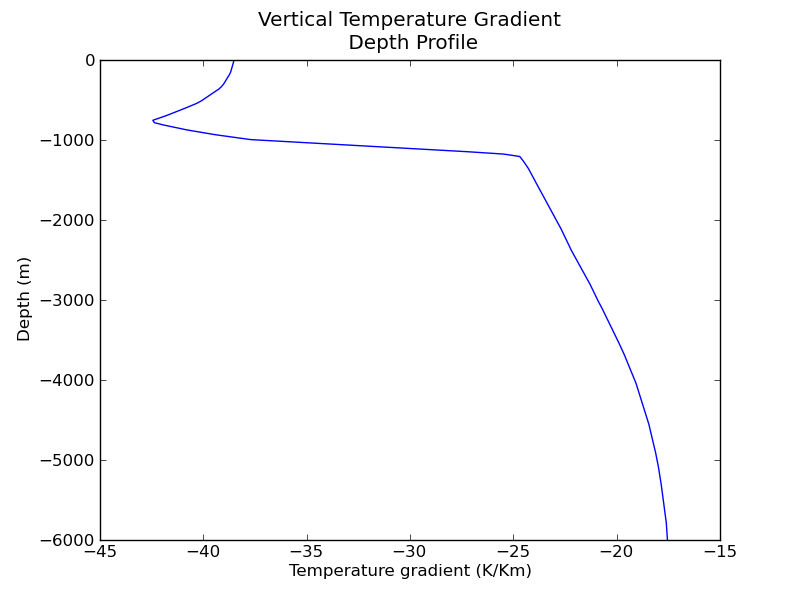
\includegraphics[width=3in]{figures/heatrefractiontgdp.png}\label{
fig:tgdp}}
    \subfigure[Thermal Conductivity
Profile]{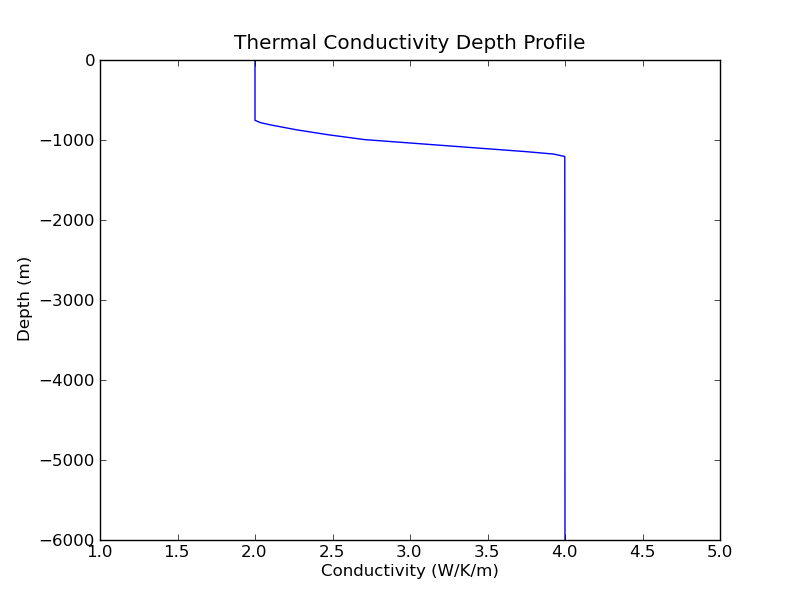
\includegraphics[width=3in]{figures/heatrefractiontcdp.png}\label{
fig:tcdp}}
    \subfigure[Heat Flow Depth
Profile]{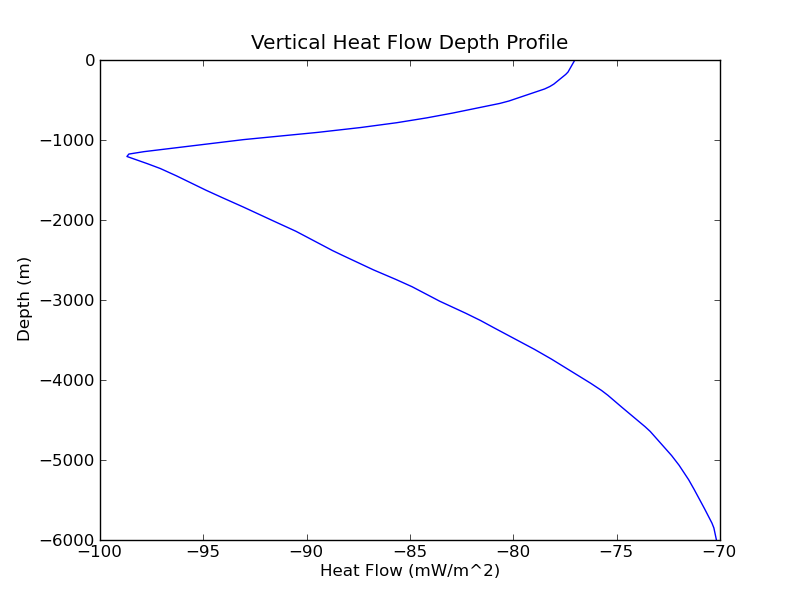
\includegraphics[width=3in]{figures/heatrefractionhf.png}\label{fig:hf}
}
  \caption{Example 5b: Depth profiles down centre of model}
  \label{figs:dps}
\end{figure}
\clearpage

\section{Arrow Plots in \mpl}
\sslist{example05c.py and cblib.py}
The distribution of the flux $-\kappa \nabla T$ is now visualised over the
domain and the results are plotted in \reffig{fig:hr001qumodel}. 
The plot puts together three components. A contour plot of the temperature,
a coloured representation of the two sub-domains where colour represents the
thermal conductivity in the particular region, and finally the arrows
representing the local direction of the steepest gradient of the flux.

Contours have already been discussed in \refSec{Sec:2DHD plot}. To show
sub-domains, we need to go back to \pycad data to get the points used to
describe the boundary of the sub-domains. We have created the \verb|CurveLoop|
class object \verb|tblockloop| to define the boundary of the upper sub-domain.
We use the \verb|getPolygon()| method of \verb|CurveLoop| to get
access to the \verb|Point|s used to define the boundary. The statement
\begin{python}
[ p.getCoordinates() for p in tblockloop.getPolygon() ]
\end{python}
creates a list of the node coordinates of all the points in question. In order 
to simplify the selection of the $x$ and $y$ coordinates the list is converted 
into \modnumpy array. To add the area coloured in brown to the plot we use; 
\begin{python}
import pylab as pl
import numarray as np
tpg=np.array([p.getCoordinates() for p in tblockloop.getPolygon() ])
pl.fill(tpg[:,0],tpg[:,1],'brown',label='2 W/m/k',zorder=-1000)
\end{python}
The same code is applied to \verb|bblockloop| to create the red area for this
sub-domain.

To plot vectors representing the flux orientation we use the 
\verb|quiver| function in \pylab. The function places vectors at locations in
the domain.
For instance one can plot vectors at the locations of the sample points used by
\esc to represent the flux \verb|-kappa*grad(T)|. As a vector is plotted at
each sample point one typically ends up with too many vectors. So one needs to
select a subset of points as follows:

First we create a coarse grid of points on a rectangular mesh, e.g. $20 \times
20$ points. Here we choose a grid of points which are located at the centre of
a \verb|nx| $\times$ \verb|ny| grid;
\begin{python}
dx = width/nx # x spacing
dy = depth/ny # y spacing
grid = [ ] # the grid points
for j in range(0,ny-1):
    for i in range(0,nx-1):
           grid.append([dx/2+dx*i,dy/2+dy*j])
\end{python}
With the \verb|Locator| function \esc provides a mechanism to identify sample
points that are closest to the grid points we have selected and to retrieve the
data at these points; 
\begin{python}
from esys.escript.pdetools import Locator
flux=-kappa*grad(T)
fluxLoc = Locator(flux.getFunctionSpace(),grid)
subflux= fluxLoc(flux) 
\end{python}
\verb|subflux| now contains a list of flux components at certain sample points.
To get the list of the sample point coordinates one can use the \verb|getX()|
method of the \verb|Locator|;
\begin{python}
subfluxloc = fluxLoc.getX()
\end{python}
To simplify the selection of $x$ and $y$ components it is convenient to
transform \verb|subflux| and \verb|subfluxloc| to \numpy arrays
\verb|xflux|, \verb|flux|.
This function is implemented in the \verb|subsample| function within the
\file{clib.py} file so we can use it in other examples. One can easily use this
function to create a vector plot of the flux;
\begin{python}
from cblib import subsample
xflux, flux=subsample(-kappa*grad(T), nx=20, ny=20)
pl.quiver(xflux[:,0],xflux[:,1],flux[:,0],flux[:,1], angles='xy',color="white")
\end{python}
Finally, we add a title and labels;
\begin{python}
pl.title("Heat Refraction across a clinal structure.")
pl.xlabel("Horizontal Displacement (m)")
pl.ylabel("Depth (m)")
pl.title("Heat Refraction across a clinal structure \n with gradient quivers.")
pl.savefig(os.path.join(saved_path,"flux.png"))
\end{python} 
to get the desired result, see \reffig{fig:hr001qumodel}.

\begin{figure}[ht]
\centerline{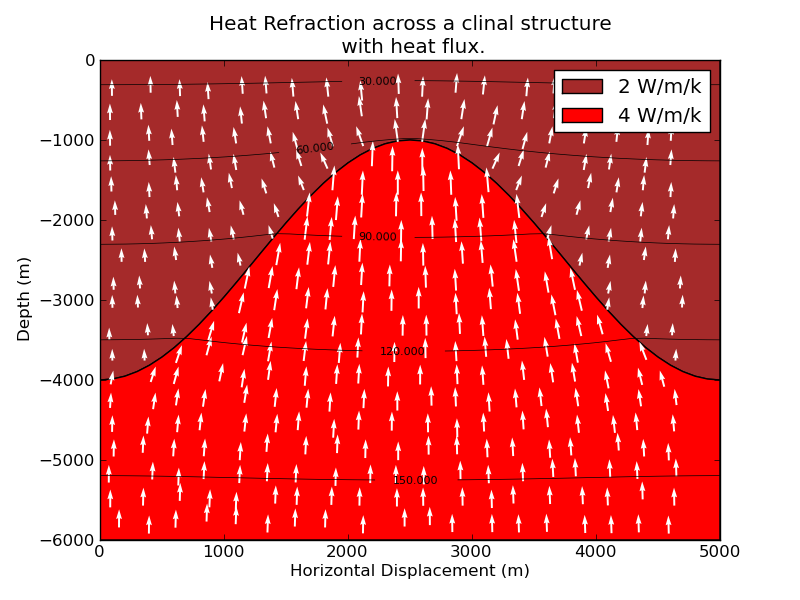
\includegraphics[width=5.in]{figures/heatrefractionflux}}
\caption{Example 5c: Heat refraction model with gradient indicated by vectors}
\label{fig:hr001qumodel}
\end{figure}
\clearpage

\section{Example 6:Fault and Overburden Model}
\sslist{example06.py and cblib.py}
A slightly more complicated model can be found in the example file
\textit{heatrefraction2_solver.py} where three blocks are used within the
model, see~\reffig{fig:hr002qumodel}. It is left to the reader to work through
this example.

\begin{figure}[ht]
\centerline{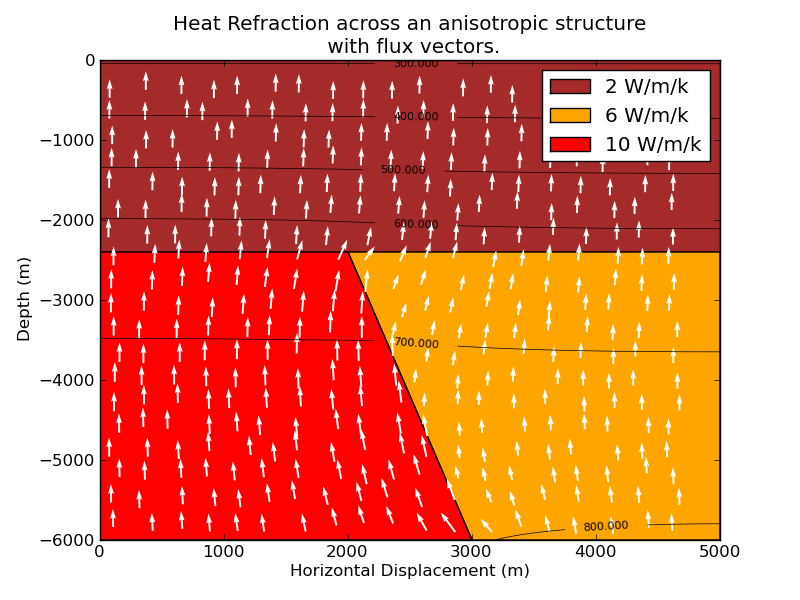
\includegraphics[width=4.in]{figures/heatrefraction2flux}}
\caption{Example 6: Heat refraction model with three blocks and heat flux}
\label{fig:hr002qumodel}
\end{figure}
\clearpage

% % % % 
% Moving into 2D and 3D wave propagations in next chapters.
% not part of release 3.1
\chapter{Acoustic Wave Propagation}

%%%%%%%%%%%%%%%%%%%%%%%%%%%%%%%%%%%%%%%%%%%%%%%%%%%%%%%%
%
% Copyright (c) 2003-2010 by University of Queensland
% Earth Systems Science Computational Center (ESSCC)
% http://www.uq.edu.au/esscc
%
% Primary Business: Queensland, Australia
% Licensed under the Open Software License version 3.0
% http://www.opensource.org/licenses/osl-3.0.php
%
%%%%%%%%%%%%%%%%%%%%%%%%%%%%%%%%%%%%%%%%%%%%%%%%%%%%%%%%



The acoustic wave equation governs the propagation of pressure waves. Wave
types that obey this law tend to travel in liquids or gases where shear waves
or longitudinal style wave motion is not possible. An obvious example is sound
waves.

The acoustic wave equation is defined as;
\begin{equation}
 \nabla ^2 p - \frac{1}{c^2} \frac{\partial ^2 p}{\partial t^2} = 0
\label{eqn:acswave}
\end{equation}
where $p$ is the pressure, $t$ is the time and $c$ is the wave velocity. In this
chapter the acoustic wave equation is demonstrated. Important steps include the
translation of the Laplacian $\nabla^2$ to the \esc general form, the stiff
equation stability criterion and solving for the displacement or acceleration solution.

\section{The Laplacian in \esc}
The Laplacian operator which can be written as $\Delta$ or $\nabla^2$,  is
calculated via the divergence of the gradient of the object, which in this
example is the scalar $p$. Thus we can write;
\begin{equation}
 \nabla^2 p = \nabla \cdot \nabla p = 
	\sum_{i}^n
	\frac{\partial^2 p}{\partial x^2_{i}}
 \label{eqn:laplacian}
\end{equation}
For the two dimensional case in Cartesian coordinates \autoref{eqn:laplacian}
becomes;
\begin{equation}
 \nabla^2 p = \frac{\partial^2 p}{\partial x^2} 
		   + \frac{\partial^2 p}{\partial y^2}
\end{equation}

In \esc the Laplacian is calculated using the divergence representation and the
intrinsic functions \textit{grad()} and \textit{trace()}. The function
\textit{grad{}} will return the spatial gradients of an object.  
For a rank 0 solution, this is of the form;
\begin{equation}
 \nabla p = \left[
	   \frac{\partial p}{\partial x _{0}},  
	   \frac{\partial p}{\partial x _{1}}
                  \right]
\label{eqn:grad}
\end{equation}
Larger ranked solution objects will return gradient tensors. For example, a
pressure field which acts in the directions $p _{0}$ and $p
_{1}$ would return;
\begin{equation}
  \nabla p = \begin{bmatrix}
	   \frac{\partial p _{0}}{\partial x _{0}} &
		\frac{\partial p _{1}}{\partial x _{0}} \\
	  \frac{\partial p _{0}}{\partial x _{1}} &
		\frac{\partial p _{1}}{\partial x _{1}} 
                  \end{bmatrix}
\label{eqn:gradrank1}
\end{equation}

\autoref{eqn:grad} corresponds to the Linear PDE general form value
$X$. Notice however, that the general form contains the term $X
_{i,j}$\footnote{This is the first derivative in the $j^{th}$
direction for the $i^{th}$ component of the solution.},
hence for a rank 0 object there is no need to do more then calculate the
gradient and submit it to the solver. In the case of the rank 1 or greater
object, it is also necessary to calculate the trace. This is the sum of the
diagonal in \autoref{eqn:gradrank1}. 

Thus when solving for equations containing the Laplacian one of two things must
be completed. If the object \verb!p! is less then rank 1 the gradient is
calculated via;
\begin{python}
gradient=grad(p)
\end{python}
and if the object is greater then or equal to a rank 1 tensor, the trace of
the gradient is calculated.
\begin{python}
 gradient=trace(grad(p))
\end{python}
These values can then be submitted to the PDE solver via the general form term
$X$. The Laplacian is then computed in the solution process by taking the
divergence of $X$.

Note, if you are unsure about the rank of your tensor, the \textit{getRank}
command will return the rank of the PDE object.
\begin{python}
 rank = p.getRank()
\end{python}


\section{Numerical Solution Stability} \label{sec:nsstab}
Unfortunately, the wave equation belongs to a class of equations called
\textbf{stiff} PDEs. These types of equations can be difficult to solve
numerically as they tend to oscillate about the exact solution, which can
eventually lead to a catastrophic failure. To counter this problem, explicitly
stable schemes like the backwards Euler method, and correct parameterisation of
the problem are required. 

There are two variables which must be considered for
stability when numerically trying to solve the wave equation. For linear media,
the two variables are related via;
\begin{equation} \label{eqn:freqvel}
f=\frac{v}{\lambda}
\end{equation}
The velocity $v$ that a wave travels in a medium is an important variable. For
stability the analytical wave must not propagate faster then the numerical wave
is able to, and in general, needs to be much slower then the numerical wave.
For example, a line 100m long is discretised into 1m intervals or 101 nodes. If
a wave enters with a propagation velocity of 100m/s then the travel time for
the wave between each node will be 0.01 seconds. The time step, must therefore
be significantly less then this. Of the order $10E-4$ would be appropriate. 
This stability criterion is known as the Courant–Friedrichs–Lewy
condition given by
\begin{equation}
dt=f\cdot \frac{dx}{v}
\end{equation}
where $dx$ is the mesh size and $f$ is a safety factor. To obtain a time step of
$10E-4$, a safety factor of $f=0.1$ was used.

The wave frequency content also plays a part in numerical stability. The
nyquist-sampling theorem states that a signals bandwidth content will be
accurately represented when an equispaced sampling rate $f _{n}$ is
equal to or greater then twice the maximum frequency of the signal
$f_{s}$, or;
\begin{equation} \label{eqn:samptheorem}
 f_{n} \geqslant f_{s}
\end{equation}
For example, a 50Hz signal will require a sampling rate greater then 100Hz or
one sample every 0.01 seconds. The wave equation relies on a spatial frequency,
thus the sampling theorem in this case applies to the solution mesh spacing.
This relationship confirms that the frequency content of the input signal
directly affects the time discretisation of the problem.

To accurately model the wave equation with high resolutions and velocities
means that very fine spatial and time discretisation is necessary for most
problems.  This requirement makes the wave equation arduous to
solve numerically due to the large number of time iterations required in each
solution. Models with very high velocities and frequencies will be the worst
affected by this problem.

\section{Displacement Solution}
\sslist{example07a.py}

We begin the solution to this PDE with the centred difference formula for the
second derivative;
\begin{equation}
 f''(x) \approx \frac{f(x+h - 2f(x) + f(x-h)}{h^2}
\label{eqn:centdiff}
\end{equation}
substituting \autoref{eqn:centdiff} for $\frac{\partial ^2 p }{\partial t ^2}$
in \autoref{eqn:acswave};
\begin{equation}
 \nabla ^2 p - \frac{1}{c^2h^2} \left[p_{(t+1)} - 2p_{(t)} +
p_{(t-1)} \right]
= 0
\label{eqn:waveu}
\end{equation}
Rearranging for $p_{(t+1)}$;
\begin{equation}
 p_{(t+1)} = c^2 h^2 \nabla ^2 p_{(t)} +2p_{(t)} -
p_{(t-1)}
\end{equation}
this can be compared with the general form of the \modLPDE module and it
becomes clear that $D=1$, $X_{i,j}=-c^2 h^2 \nabla ^2 p_{(t)}$ and
$Y=2p_{(t)} - p_{(t-1)}$.

The solution script is similar to others that we have created in previous
chapters. The general steps are;
\begin{enumerate}
 \item The necessary libraries must be imported.
 \item The domain needs to be defined.
 \item The time iteration and control parameters need to be defined.
 \item The PDE is initialised with source and boundary conditions.
 \item The time loop is started and the PDE is solved at consecutive time steps.
 \item All or select solutions are saved to file for visualisation later on.
\end{enumerate}

Parts of the script which warrant more attention are the definition of the
source, visualising the source, the solution time loop and the VTK data export.

\subsection{Pressure Sources}
As the pressure is a scalar, one need only define the pressure for two 
time steps prior to the start of the solution loop. Two known solutions are
required because the wave equation contains a double partial derivative with
respect to time. This is often a good opportunity to introduce a source to the
solution. This model has the source located at it's centre. The source should
be smooth and cover a number of samples to satisfy the frequency stability
criterion. Small sources will generate high frequency signals. Here, when using
a rectangular domain, the source is defined by a cosine function.
\begin{python}
U0=0.01 # amplitude of point source
xc=[500,500] #location of point source
# define small radius around point xc
src_radius = 30
# for first two time steps
u=U0*(cos(length(x-xc)*3.1415/src_radius)+1)*\
	whereNegative(length(x-xc)-src_radius)
u_m1=u
\end{python}

\subsection{Visualising the Source}
There are two options for visualising the source. The first is to export the
initial conditions of the model to VTK, which can be interpreted as a scalar
surface in Mayavi2. The second is to take a cross section of the model which
will require the \textit{Locator} function. 
First \verb!Locator! must be imported;
\begin{python}
 from esys.escript.pdetools import Locator
\end{python}
The function can then be used on the domain to locate the nearest domain node
to the point or points of interest.

It is now necessary to build a list of $(x,y)$ locations that specify where are
model slice will go. This is easily implemented with a loop;
\begin{python}
cut_loc=[]
src_cut=[]
for i in range(ndx/2-ndx/10,ndx/2+ndx/10):
    cut_loc.append(xstep*i)
    src_cut.append([xstep*i,xc[1]])
\end{python}
We then submit the output to \verb!Locator! and finally return the appropriate
values using the \verb!getValue! function.
\begin{python}
src=Locator(mydomain,src_cut)
src_cut=src.getValue(u)
\end{python}
It is then a trivial task to plot and save the output using \mpl
(\autoref{fig:cxsource}).
\begin{python}
pl.plot(cut_loc,src_cut)
pl.axis([xc[0]-src_radius*3,xc[0]+src_radius*3,0.,2*U0])
pl.savefig(os.path.join(savepath,"source_line.png"))
\end{python}
\begin{figure}[h]
 \centering
	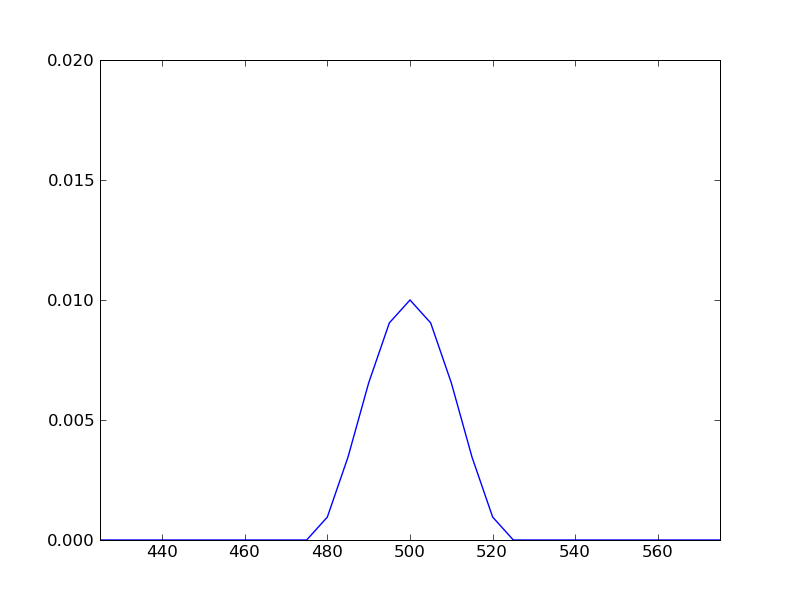
\includegraphics[width=6in]{figures/sourceline.png}
 \caption{Cross section of the source function.}
 \label{fig:cxsource}
\end{figure}


\subsection{Point Monitoring}
In the more general case where the solution mesh is irregular or specific
locations need to be monitored, it is simple enough to use the \textit{Locator}
function. 
\begin{python}
 rec=Locator(mydomain,[250.,250.])
\end{python}
 When the solution \verb u  is updated we can extract the value at that point
via;
\begin{python}
 u_rec=rec.getValue(u)
\end{python}
For consecutive time steps one can record the values from \verb!u_rec! in an
array initialised as \verb!u_rec0=[]! with;
\begin{python}
  u_rec0.append(rec.getValue(u))
\end{python}

It can be useful to monitor the value at a single or multiple individual points
in the model during the modelling process. This is done using 
the \verb!Locator! function.


\section{Acceleration Solution}
\sslist{example07b.py}

An alternative method to the displacement solution, is to solve for the
acceleration $\frac{\partial ^2 p}{\partial t^2}$ directly. The displacement can
then be derived from the acceleration after a solution has been calculated
The acceleration is given by a modified form of \autoref{eqn:waveu};
\begin{equation}
  \nabla ^2 p - \frac{1}{c^2} a = 0
\label{eqn:wavea}
\end{equation}
and can be solved directly with $Y=0$ and $X=-c^2 \nabla ^2 p_{(t)}$.
After each iteration the displacement is re-evaluated via;
\begin{equation}
 p_{(t+1)}=2p_{(t)} - p_{(t-1)} + h^2a
\end{equation}

\subsection{Lumping}
For \esc, the acceleration solution is prefered as it allows the use of matrix
lumping. Lumping or mass lumping as it is sometimes known, is the process of
aggressively approximating the density elements of a mass matrix into the main
diagonal. The use of Lumping is motivaed by the simplicity of diagonal matrix
 inversion. As a result, Lumping can significantly reduce the computational
requirements of a problem. Care should be taken however, as this
function can only be used when the $A$, $B$ and $C$ coefficients of the
general form are zero. 

More information about the lumping implementation used in \esc and its accuracy
can be found in the user guide.

To turn lumping on in \esc one can use the command;
\begin{python}
 mypde.getSolverOptions().setSolverMethod(mypde.getSolverOptions().HRZ_LUMPING)
\end{python}
It is also possible to check if lumping is set using;
\begin{python}
  print mypde.isUsingLumping()
\end{python}

\section{Stability Investigation}
It is now prudent to investigate the stability limitations of this problem.
First, we let the frequency content of the source be very small. If we define
the source as a cosine input, then the wavlength of the input is equal to the
radius of the source. Let this value be 5 meters. Now, if the maximum velocity
of the model is $c=380.0ms^{-1}$, then the source
frequency is $f_{r} = \frac{380.0}{5} = 76.0 Hz$. This is a worst case
scenario with a small source and the models maximum velocity. 

Furthermore, we know from \autoref{sec:nsstab}, that the spatial sampling
frequency must be at least twice this value to ensure stability. If we assume
the model mesh is a square equispaced grid,
then the sampling interval is the side length divided by the number of samples,
given by $\Delta x = \frac{1000.0m}{400} = 2.5m$ and the maximum sampling
frequency capable at this interval is
$f_{s}=\frac{380.0ms^{-1}}{2.5m}=152Hz$ this is just equal to the
required rate satisfying \autoref{eqn:samptheorem}. 

\autoref{fig:ex07sampth} depicts three examples where the grid has been
undersampled, sampled correctly, and over sampled. The grids used had
200, 400 and 800 nodes per side respectively. Obviously, the oversampled grid
retains the best resolution of the modelled wave.

The time step required for each of these examples is simply calculated from
the propagation requirement. For a maximum velocity of $380.0ms^{-1}$,
\begin{subequations}
 \begin{equation}
  \Delta t \leq \frac{1000.0m}{200} \frac{1}{380.0} = 0.013s
 \end{equation}
 \begin{equation}
  \Delta t \leq \frac{1000.0m}{400} \frac{1}{380.0} = 0.0065s
 \end{equation}
 \begin{equation}
  \Delta t \leq \frac{1000.0m}{800} \frac{1}{380.0} = 0.0032s
 \end{equation}
\end{subequations}
Observe that for each doubling of the number of nodes in the mesh, we halve
the time step. To illustrate the impact this has, consider our model. If the
source is placed at the center, it is $500m$ from the nearest boundary. With a
velocity of $380.0ms^{-1}$ it will take $\approx1.3s$ for the wavefront to
reach that boundary. In each case, this equates to $100$,  $200$ and $400$ time
steps. This is again, only a best case scenario, for true stability these time
values may need to be halved and possibly halved again.

\begin{figure}[ht]
\centering
\subfigure[Undersampled Example]{
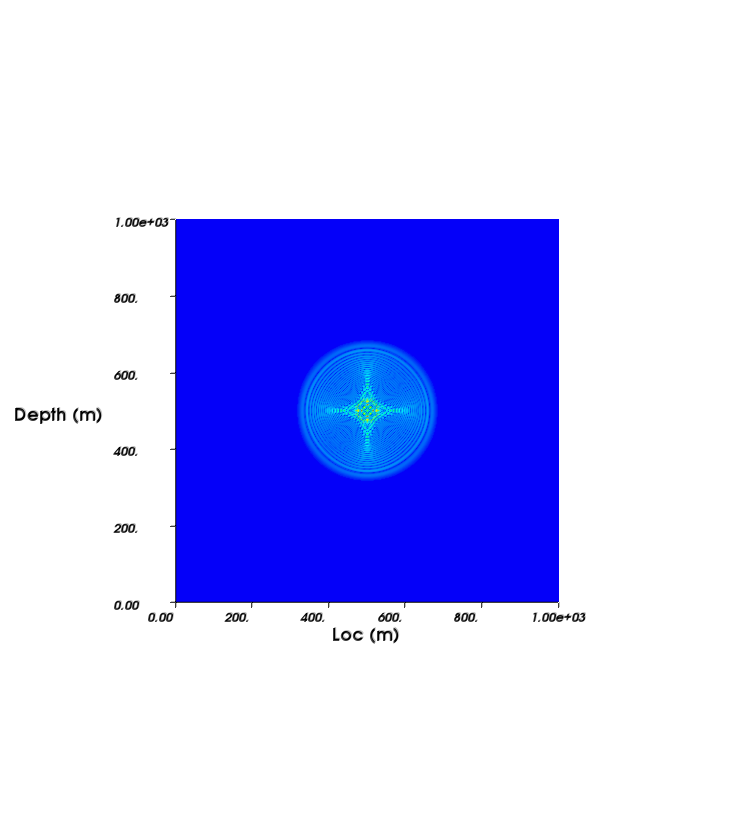
\includegraphics[width=0.45\textwidth,trim=0cm 6cm 5cm 6cm
,clip]{figures/ex07usamp.png}
\label{fig:ex07usamp}
}
\subfigure[Just sampled Example]{
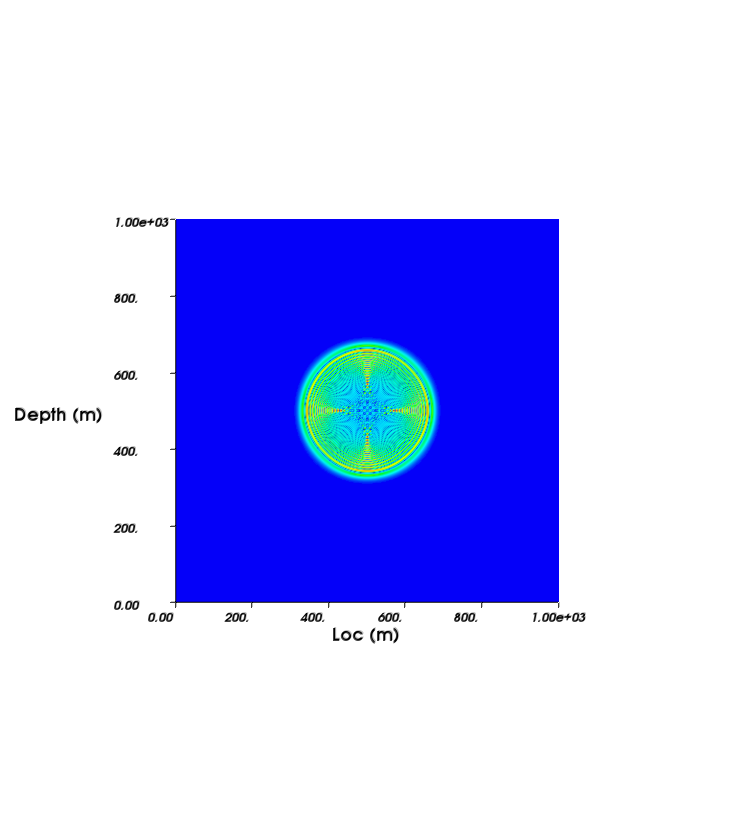
\includegraphics[width=0.45\textwidth,trim=0cm 6cm 5cm 6cm
,clip]{figures/ex07jsamp.png}
\label{fig:ex07jsamp}
}
\subfigure[Over sampled Example]{
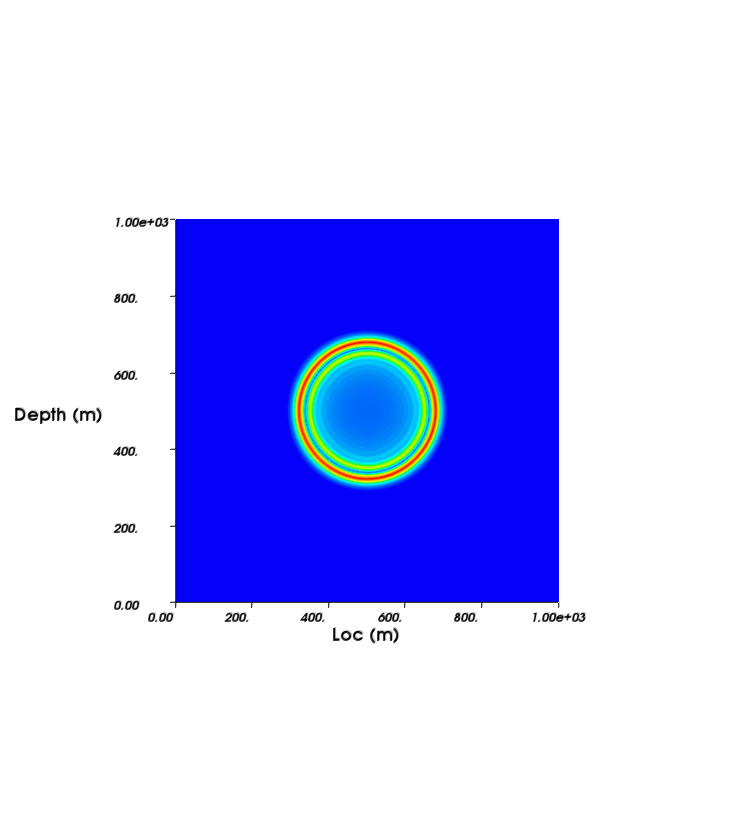
\includegraphics[width=0.45\textwidth,trim=0cm 6cm 5cm 6cm
,clip]{figures/ex07nsamp.png}
\label{fig:ex07nsamp}
}
\caption{Sampling Theorem example for stability
investigation.}
\label{fig:ex07sampth}
\end{figure}



 

 %acoustic wave equation
% 
\chapter{Seismic Wave Propagation}
 
%%%%%%%%%%%%%%%%%%%%%%%%%%%%%%%%%%%%%%%%%%%%%%%%%%%%%%%%%%%%%%%%%%%%%%%%%%%%%%
% Copyright (c) 2003-2016 by The University of Queensland
% http://www.uq.edu.au
%
% Primary Business: Queensland, Australia
% Licensed under the Open Software License version 3.0
% http://www.opensource.org/licenses/osl-3.0.php
%
% Development until 2012 by Earth Systems Science Computational Center (ESSCC)
% Development 2012-2013 by School of Earth Sciences
% Development from 2014 by Centre for Geoscience Computing (GeoComp)
%
%%%%%%%%%%%%%%%%%%%%%%%%%%%%%%%%%%%%%%%%%%%%%%%%%%%%%%%%%%%%%%%%%%%%%%%%%%%%%%

\section{Seismic Wave Propagation in Two Dimensions}

\sslist{example08a.py}
We will now expand upon the previous chapter by introducing a vector form of
the wave equation. This means that the waves will have not only a scalar
magnitude as for the pressure wave solution, but also a direction. This type of
scenario is apparent in wave types that exhibit compressional and transverse
particle motion. An example of this would be seismic waves.

Wave propagation in the earth can be described by the elastic wave equation
\begin{equation} \label{eqn:wav} \index{wave equation}
\rho \frac{\partial^{2}u_{i}}{\partial t^2} - \frac{\partial
\sigma_{ij}}{\partial x_{j}} = 0
\end{equation}
where $\sigma$ is the stress given by
\begin{equation} \label{eqn:sigw}
 \sigma _{ij} = \lambda u_{k,k} \delta_{ij} + \mu (
u_{i,j} + u_{j,i})
\end{equation}
and $\lambda$ and $\mu$ represent Lame's parameters. Specifically for seismic
waves, $\mu$ is the propagation materials shear modulus. 
In a similar process to the previous chapter, we will use the acceleration
solution to solve this PDE. By substituting $a$ directly for
$\frac{\partial^{2}u_{i}}{\partial t^2}$ we can derive the
acceleration solution. Using $a$ we can see that \autoref{eqn:wav} becomes
\begin{equation} \label{eqn:wava} 
\rho a_{i} - \frac{\partial
\sigma_{ij}}{\partial x_{j}} = 0
\end{equation}
Thus the problem will be solved for acceleration and then converted to 
displacement using the backwards difference approximation as for the acoustic
example in the previous chapter.

Consider now the stress $\sigma$. One can see that the stress consists of two
distinct terms:
\begin{subequations}
\begin{equation} \label{eqn:sigtrace}
\lambda u_{k,k} \delta_{ij}
\end{equation}
\begin{equation} \label{eqn:sigtrans}
\mu (u_{i,j} + u_{j,i})
\end{equation}
\end{subequations}
One simply recognizes in \autoref{eqn:sigtrace} that $u_{k,k}$ is the
trace of the displacement solution and that $\delta_{ij}$ is the
kronecker delta function with dimensions equivalent to $u$. The second term
\autoref{eqn:sigtrans} is the sum of $u$ with its own transpose. Putting these
facts together we see that the spatial differential of the stress is given by the
gradient of $u$ and the aforementioned operations. This value is then submitted
to the \esc PDE as $X$.
\begin{python}
g=grad(u); stress=lam*trace(g)*kmat+mu*(g+transpose(g))
mypde.setValue(X=-stress) # set PDE values
\end{python}
The solution is then obtained via the usual method and the displacement is
calculated so that the memory variables can be updated for the next time
iteration.
\begin{python}
accel = mypde.getSolution() #get PDE solution for acceleration
u_p1=(2.*u-u_m1)+h*h*accel #calculate displacement
u_m1=u; u=u_p1 # shift values by 1
\end{python}

Saving the data has been handled slightly differently in this example. The VTK
files generated can be quite large and take a significant amount of time to save
to the hard disk. To avoid doing this at every iteration a test is devised which
saves only at specific time intervals.

To do this there are two new parameters in our script.
\begin{python}
# data recording times
rtime=0.0 # first time to record
rtime_inc=tend/20.0 # time increment to record
\end{python}
Currently the PDE solution will be saved to file $20$ times between the start of
the modelling and the final time step. With these parameters set, an if
statement is introduced to the time loop
\begin{python}
if (t >= rtime):
	saveVTK(os.path.join(savepath,"ex08a.%05d.vtu"%n),displacement=length(u),\
    	acceleration=length(accel),tensor=stress)
    	rtime=rtime+rtime_inc #increment data save time
\end{python}
\verb!t! is the time counter. Whenever the recording time \verb!rtime! is less
then \verb!t! the solution is saved and \verb!rtime! is incremented. This
limits the number of outputs and increases the speed of the solver.

\section{Multi-threading}
The wave equation solution can be quite demanding on CPU time. Enhancements can
be made by accessing multiple threads or cores on your computer. This does not
require any modification to the solution script and only comes into play when
\esc is called from the shell. To use multiple threads \esc is called using
the \verb!-t! option with an integer argument for the number of threads
required. For example
\begin{verbatim}
$escript -t 4 example08a.py
\end{verbatim}
would call the script in this section and solve it using 4 threads.

The computation times on an increasing number of cores is outlined in
\autoref{tab:wpcores}.

\begin{table}[ht]
\begin{center}
\caption{Computation times for an increasing number of cores.}
\label{tab:wpcores}
\begin{tabular}{| c | c |}
\hline
Number of Cores & Time (s) \\
\hline
1 & 691.0 \\
2 & 400.0 \\
3 & 305.0 \\
4 & 328.0 \\
5 & 323.0 \\
6 & 292.0 \\
7 & 282.0 \\
8 & 445.0 \\ \hline
\end{tabular}
\end{center}
\end{table}

\section{Vector source on the boundary}
\sslist{example08b.py}
For this particular example, we will introduce the source by applying a
displacement to the boundary during the initial time steps. The source will
again be
a radially propagating wave but due to the vector nature of the PDE used, a
direction will need to be applied to the source.

The first step is to choose an amplitude and create the source as in the
previous chapter. 
\begin{python}
U0=0.01 # amplitude of point source
# will introduce a spherical source at middle left of bottom face
xc=[ndx/2,0]

############################################FIRST TIME STEPS AND SOURCE
# define small radius around point xc
src_length = 40; print("src_length = ",src_length)
# set initial values for first two time steps with source terms
xb=FunctionOnBoundary(domain).getX()
y=source[0]*(cos(length(x-xc)*3.1415/src_length)+1)*\
                whereNegative(length(xb-src_length))
src_dir=numpy.array([0.,1.]) # defines direction of point source as down
y=y*src_dir
\end{python}
where \verb xc  is the source point on the boundary of the model. Note that
because the source is specifically located on the boundary, we have used the
\verb!FunctionOnBoundary! call to ensure the nodes used to define the source
are also located upon the boundary. These boundary nodes are passed to
source as \verb!xb!. The source direction is then defined as an $(x,y)$ array and multiplied by the 
source function. The directional array must have a magnitude of $\left| 1
\right| $ otherwise the amplitude of the source will become modified. For this
example, the source is directed in the $-y$ direction.
\begin{python}
src_dir=numpy.array([0.,-1.]) # defines direction of point source as down
y=y*src_dir
\end{python}
The function can then be applied as a boundary condition by setting it equal to
$y$ in the general form.
\begin{python}
mypde.setValue(y=y) #set the source as a function on the boundary
\end{python}
The final step is to qualify the initial conditions. Due to the fact that we are
no longer using the source to define our initial condition to the model, we
must set the model state to zero for the first two time steps.
\begin{python}
# initial value of displacement at point source is constant (U0=0.01)
# for first two time steps
u=[0.0,0.0]*wherePositive(x)
u_m1=u
\end{python}

If the source is time progressive, $y$ can be updated during the
iteration stage. This is covered in the following section.

\begin{figure}[htp]
\centering
\subfigure[Example 08a at 0.025s ]{
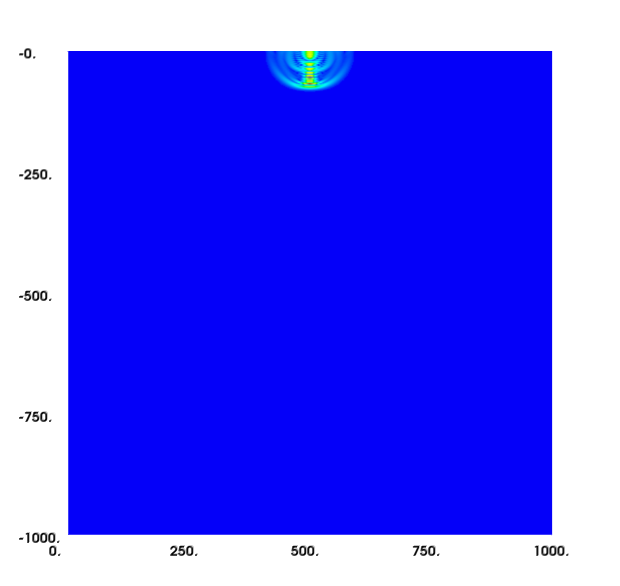
\includegraphics[width=3in]{figures/ex08pw50.png}
\label{fig:ex08pw50}
}
\subfigure[Example 08a at 0.175s ]{
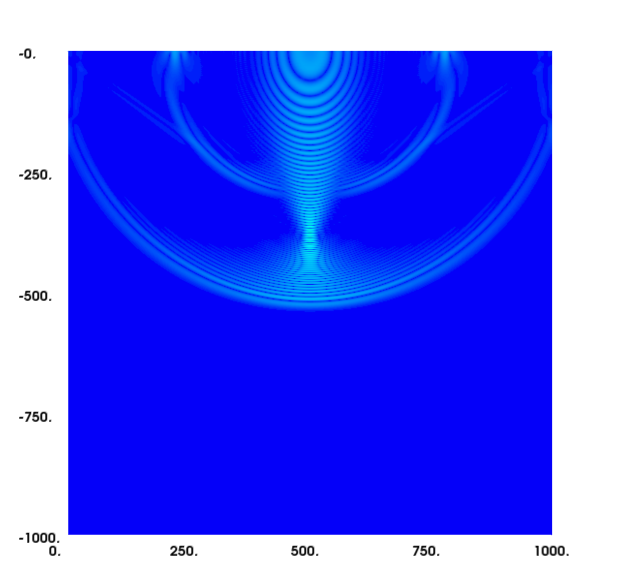
\includegraphics[width=3in]{figures/ex08pw350.png}
\label{fig:ex08pw350}
} \\
\subfigure[Example 08a at 0.325s ]{
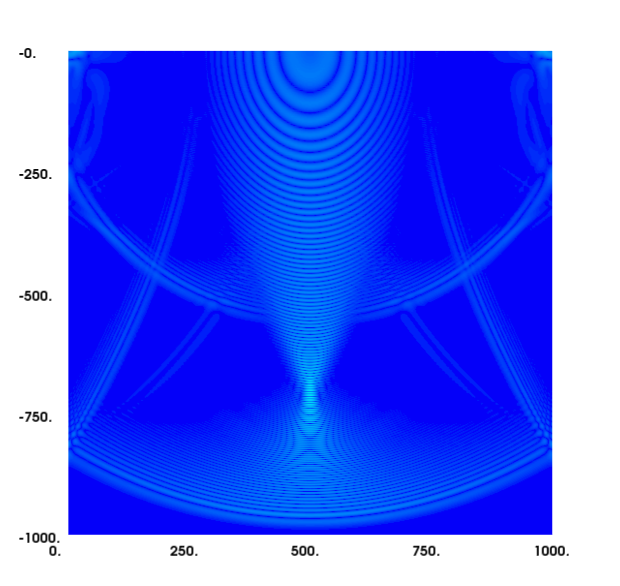
\includegraphics[width=3in]{figures/ex08pw650.png}
\label{fig:ex08pw650}
}
\subfigure[Example 08a at 0.475s ]{
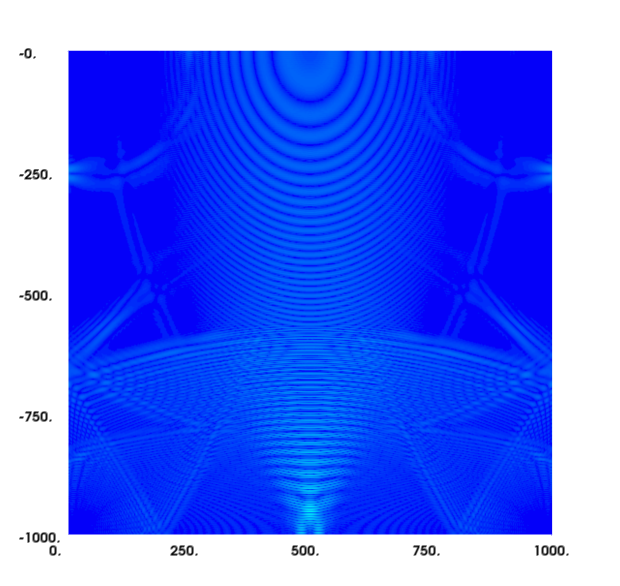
\includegraphics[width=3in]{figures/ex08pw950.png}
\label{fig:ex08pw950}
}
\label{fig:ex08pw}
\caption{Results of Example 08 at various times.}
\end{figure}
\clearpage

\section{Time variant source}

\sslist{example08b.py}
Until this point, all of the wave propagation examples in this cookbook have
used impulsive sources which are smooth in space but not time. It is however,
advantageous to have a time smoothed source as it can reduce the temporal
frequency range and thus mitigate aliasing in the solution. 

It is quite 
simple to implement a source which is smooth in time. In addition to the
original source function the only extra requirement is a time function. For
this example the time variant source will be the derivative of a Gaussian curve
defined by the required dominant frequency (\autoref{fig:tvsource}).
\begin{python}
#Creating the time function of the source.
dfeq=50 #Dominant Frequency
a = 2.0 * (np.pi * dfeq)**2.0
t0 = 5.0 / (2.0 * np.pi * dfeq)
srclength = 5. * t0
ls = int(srclength/h)
print('source length',ls)
source=np.zeros(ls,'float') # source array
ampmax=0
for it in range(0,ls):
    t = it*h
    tt = t-t0
    dum1 = np.exp(-a * tt * tt)
    source[it] = -2. * a * tt * dum1
    if (abs(source[it]) > ampmax):
        ampmax = abs(source[it])
    time[t]=t*h
\end{python}
\begin{figure}[ht]
\centering
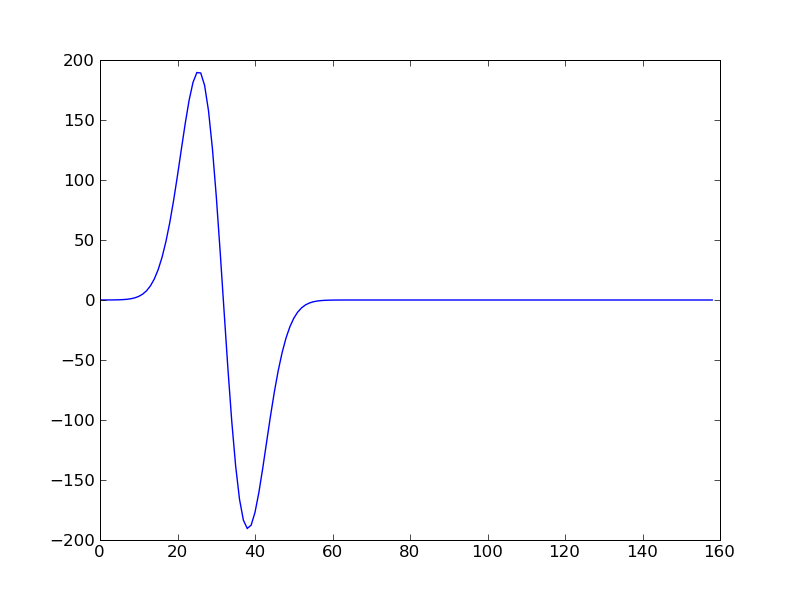
\includegraphics[width=3in]{figures/source.png}
\caption{Time variant source with a dominant frequency of 50Hz.}
\label{fig:tvsource}
\end{figure}

We then build the source and the first two time steps via;
\begin{python}
# set initial values for first two time steps with source terms
y=source[0]
*(cos(length(x-xc)*3.1415/src_length)+1)*whereNegative(length(x-xc)-src_length)
src_dir=numpy.array([0.,-1.]) # defines direction of point source as down
y=y*src_dir
mypde.setValue(y=y) #set the source as a function on the boundary
# initial value of displacement at point source is constant (U0=0.01)
# for first two time steps
u=[0.0,0.0]*whereNegative(x)
u_m1=u
\end{python}

Finally, for the length of the source, we are required to update each new
solution in the iterative section of the solver. This is done via;
\begin{python}
# increment loop values
t=t+h; n=n+1
if (n < ls):
	y=source[n]**(cos(length(x-xc)*3.1415/src_length)+1)*\
                   whereNegative(length(x-xc)-src_length)
        y=y*src_dir; mypde.setValue(y=y) #set the source as a function on the
boundary
\end{python}

\section{Absorbing Boundary Conditions}
To mitigate the effect of the boundary on the model, absorbing boundary
conditions can be introduced. These conditions effectively dampen the wave energy
as they approach the boundary and thus prevent that energy from being reflected.
This type of approach is typically used when a model is shrunk to decrease
computational requirements. In practise this applies to almost all models,
especially in earth sciences where the entire planet or a large enough
portional of it cannot be modelled efficiently when considering small scale
problems. It is impractical to calculate the solution for an infinite model and thus ABCs allow
us the create an approximate solution with small to zero boundary effects on a
model with a solvable size.

To dampen the waves, the method of \citet{Cerjan1985}
where the solution and the stress are multiplied by a damping function defined
on $n$ nodes of the domain adjacent to the boundary, given by;
\begin{equation}
\gamma =\sqrt{\frac{| -log( \gamma _{b} ) |}{n^2}}
\end{equation}
\begin{equation}
y=e^{-(\gamma x)^2}
\end{equation}
This is applied to the bounding 20-50 pts of the model using the location
specifiers of \esc;
\begin{python}
# Define where the boundary decay will be applied.
bn=30.
bleft=xstep*bn; bright=mx-(xstep*bn); bbot=my-(ystep*bn)
# btop=ystep*bn # don't apply to force boundary!!!

# locate these points in the domain
left=x[0]-bleft; right=x[0]-bright; bottom=x[1]-bbot

tgamma=0.98   # decay value for exponential function
def calc_gamma(G,npts):
    func=np.sqrt(abs(-1.*np.log(G)/(npts**2.)))
    return func

gleft  = calc_gamma(tgamma,bleft)
gright = calc_gamma(tgamma,bleft)
gbottom= calc_gamma(tgamma,ystep*bn)

print('gamma', gleft,gright,gbottom)

# calculate decay functions
def abc_bfunc(gamma,loc,x,G):
    func=exp(-1.*(gamma*abs(loc-x))**2.)
    return func

fleft=abc_bfunc(gleft,bleft,x[0],tgamma)
fright=abc_bfunc(gright,bright,x[0],tgamma)
fbottom=abc_bfunc(gbottom,bbot,x[1],tgamma)
# apply these functions only where relevant
abcleft=fleft*whereNegative(left)
abcright=fright*wherePositive(right)
abcbottom=fbottom*wherePositive(bottom)
# make sure the inside of the abc is value 1
abcleft=abcleft+whereZero(abcleft)
abcright=abcright+whereZero(abcright)
abcbottom=abcbottom+whereZero(abcbottom)
# multiply the conditions together to get a smooth result
abc=abcleft*abcright*abcbottom
\end{python}
Note that the boundary conditions are not applied to the surface, as this is
effectively a free surface where normal reflections would be experienced.
Special conditions can be introduced at this surface if they are known. The
resulting boundary damping function can be viewed in
\autoref{fig:abconds}.

\section{Second order Meshing}
For stiff problems like the wave equation it is often prudent to implement
second order meshing. This creates a more accurate mesh approximation with some
increased processing cost. To turn second order meshing on, the \verb!rectangle!
function accepts an \verb!order! keyword argument.
\begin{python}
domain=Rectangle(l0=mx,l1=my,n0=ndx, n1=ndy,order=2) # create the domain
\end{python}
Other pycad functions and objects have similar keyword arguments for higher
order meshing.

Note that when implementing second order meshing, a smaller timestep is required
then for first order meshes as the second order essentially reduces the size of
the mesh by half.

\begin{figure}[ht]
 \centering
 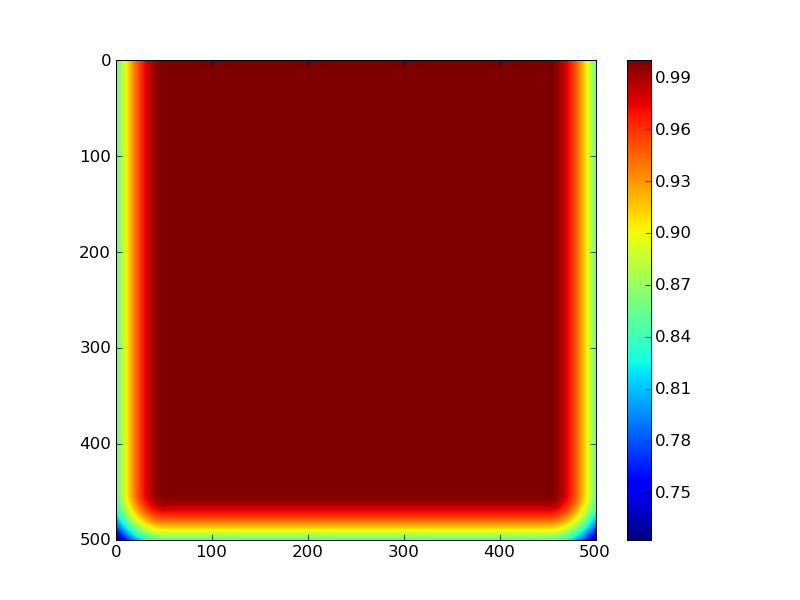
\includegraphics[width=5in]{figures/ex08babc.png}
 \label{fig:abconds}
 \caption{Absorbing boundary conditions for example08b.py}
\end{figure}

\begin{figure}[htp]
\centering
\subfigure[Example 08b at 0.03s ]{
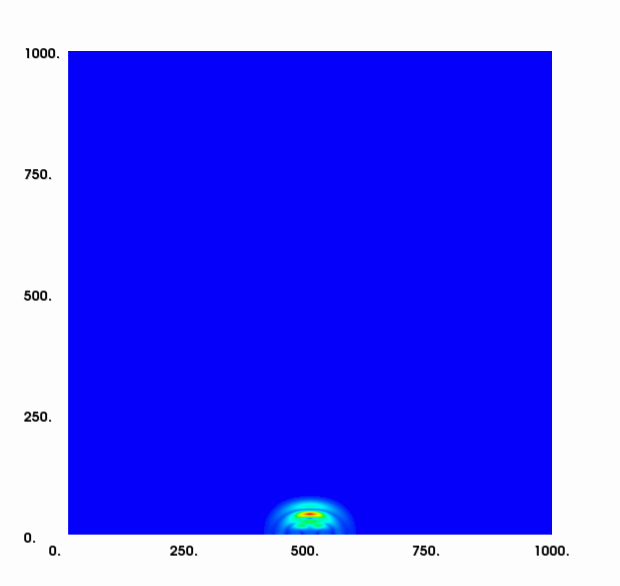
\includegraphics[width=3in]{figures/ex08sw060.png}
\label{fig:ex08pw060}
}
\subfigure[Example 08b at 0.16s ]{
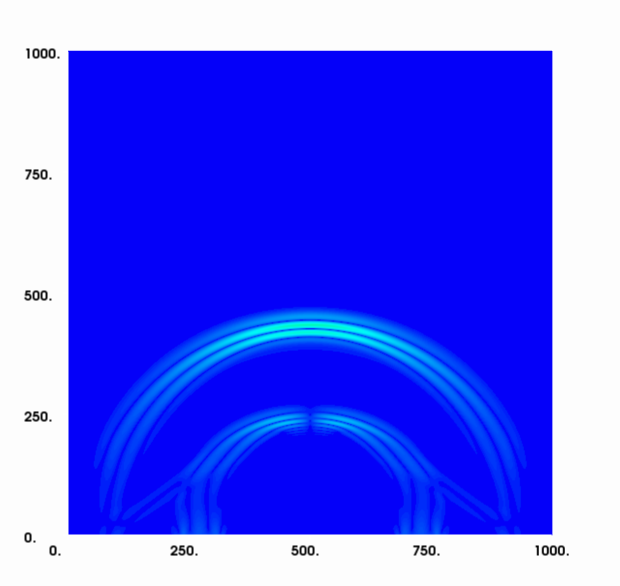
\includegraphics[width=3in]{figures/ex08sw320.png}
\label{fig:ex08pw320}
} \\
\subfigure[Example 08b at 0.33s ]{
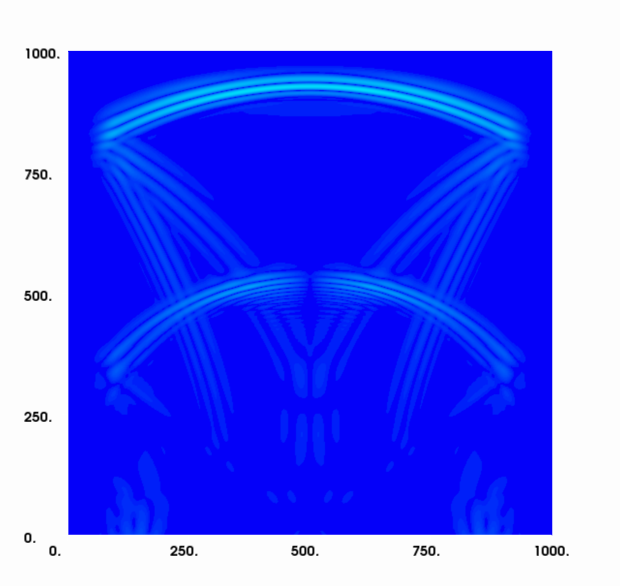
\includegraphics[width=3in]{figures/ex08sw660.png}
\label{fig:ex08pw660}
}
\subfigure[Example 08b at 0.44s ]{
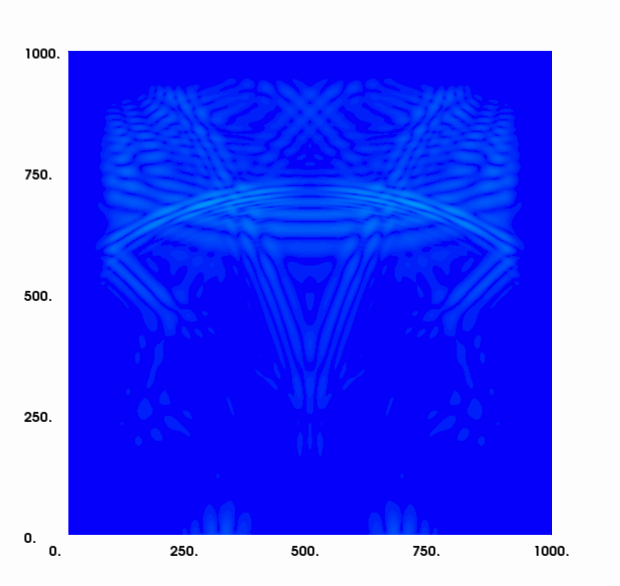
\includegraphics[width=3in]{figures/ex08sw880.png}
\label{fig:ex08pw880}
}
\label{fig:ex08pw}
\caption{Results of Example 08b at various times.}
\end{figure}
\clearpage

\section{Pycad example}
\sslist{example08c.py}
To make the problem more interesting we will now introduce an interface to the
middle of the domain. In fact we will use the same domain as we did fora
different set of material properties on either side of the interface.

\begin{figure}[ht]
\begin{center}
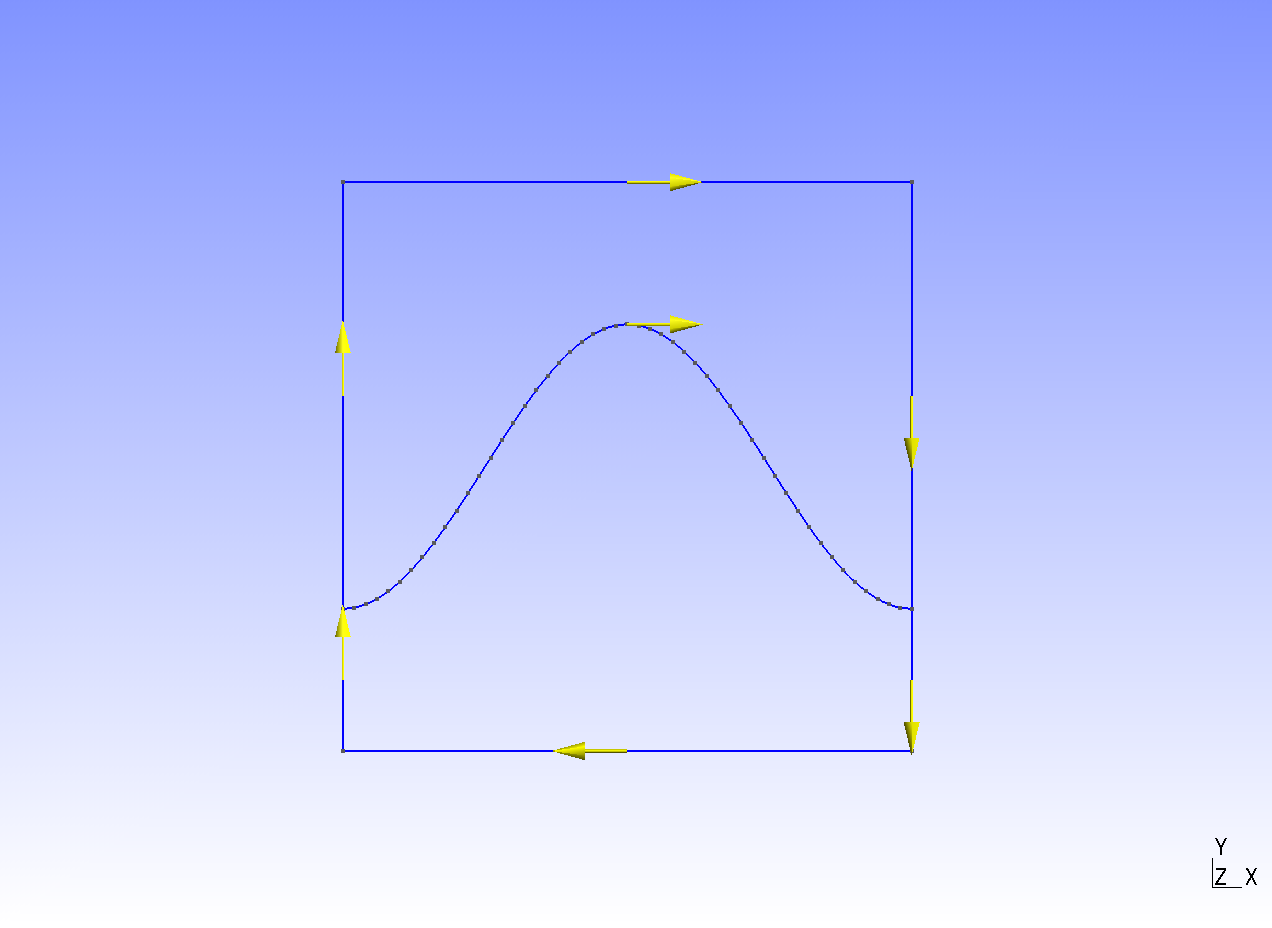
\includegraphics[width=5in]{figures/gmsh-example08c.png}
\caption{Domain geometry for example08c.py showing line tangents.}
\label{fig:ex08cgeo}
\end{center}
\end{figure}

It is simple enough to slightly modify the scripts of the previous sections to
accept this domain. Multiple material parameters must now be defined and assigned
to specific tagged areas. Again this is done via
\begin{python}
lam=Scalar(0,Function(domain))
lam.setTaggedValue("top",lam1)
lam.setTaggedValue("bottom",lam2)
mu=Scalar(0,Function(domain))
mu.setTaggedValue("top",mu1)
mu.setTaggedValue("bottom",mu2)
rho=Scalar(0,Function(domain))
rho.setTaggedValue("top",rho1)
rho.setTaggedValue("bottom",rho2)
\end{python}
Don't forget that the source boundary must also be tagged and added so it can
be referenced 
\begin{python}
# Add the subdomains and flux boundaries.
d.addItems(PropertySet("top",tblock),PropertySet("bottom",bblock),\
                                     PropertySet("linetop",l30))
\end{python}
It is now possible to solve the script as in the previous examples
(\autoref{fig:ex08cres}).

\begin{figure}[ht]
\centering
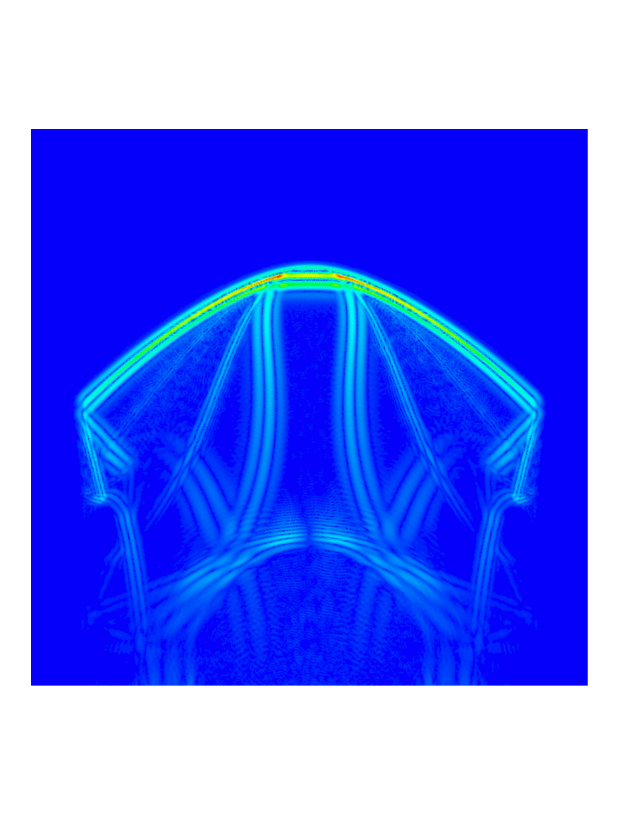
\includegraphics[width=4in]{figures/ex08c2601.png}
\caption{Modelling results of example08c.py at 0.2601 seconds. Notice the
refraction of the wave front about the boundary between the two layers.}
\label{fig:ex08cres}
\end{figure}




\chapter{3D Seismic Wave Propagation}
 
%%%%%%%%%%%%%%%%%%%%%%%%%%%%%%%%%%%%%%%%%%%%%%%%%%%%%%%%%%%%%%%%%%%%%%%%%%%%%%
% Copyright (c) 2003-2013 by University of Queensland
% http://www.uq.edu.au
%
% Primary Business: Queensland, Australia
% Licensed under the Open Software License version 3.0
% http://www.opensource.org/licenses/osl-3.0.php
%
% Development until 2012 by Earth Systems Science Computational Center (ESSCC)
% Development since 2012 by School of Earth Sciences
%
%%%%%%%%%%%%%%%%%%%%%%%%%%%%%%%%%%%%%%%%%%%%%%%%%%%%%%%%%%%%%%%%%%%%%%%%%%%%%%

\section{3D pycad}
\sslist{example09m.py}
This example explains how to build a 3D layered domain using pycad. As
simple as this example sounds, there are a few import concepts that one must
remember  so that the model will function correctly.
\begin{itemize}
  \item There must be no duplication of any geometric features whether they are
  points, lines, loops, surfaces or volumes.
  \item All objects with dimensions greater then a line have a normal defined by
  the right hand rule (RHR). It is important to consider which direction a
  normal is oriented when combining primitives to form higher order shapes.
\end{itemize}

The first step as always is to import the external modules. To build a 3D model
and mesh we will need pycad, some GMesh interfaces, the Finley domain builder
and some additional tools.
\begin{python}
#######################################################EXTERNAL MODULES
from esys.pycad import * #domain constructor
from esys.pycad.gmsh import Design #Finite Element meshing package
from esys.finley import MakeDomain #Converter for escript
from esys.escript import mkDir, getMPISizeWorld
import os
\end{python}
After carrying out some routine checks and setting the \verb!save_path! we then
specify the parameters of the model. This model will be 2000 by 2000 meters on
the surface and extend to a depth of 500 meters. An interface or boundary
between two layers will be created at half the total depth or 250 meters. This
type of model is known as a horizontally layered model or a layer cake model. 
\begin{python}
################################################ESTABLISHING PARAMETERS
#Model Parameters
xwidth=2000.0*m   #x width of model
ywidth=2000.0*m   #y width of model
depth=500.0*m   #depth of model
intf=depth/2.   #Depth of the interface.
\end{python}
We now start to specify the components of our model starting with the vertexes
using the \verb!Point! primitive. These are then joined by lines in a regular
manner taking note of the right hand rule. Finally, the lines are turned into
loops and then planar surfaces.
\footnote{Some code has been emmitted here for
simlpicity. For the full script please refer to the script referenced at the beginning of
this section.}
\begin{python}
####################################################DOMAIN CONSTRUCTION
# Domain Corners
p0=Point(0.0,    0.0,      0.0)
#..etc..
l45=Line(p4, p5)

# Join line segments to create domain boundaries and then surfaces
ctop=CurveLoop(l01, l12, l23, l30);     stop=PlaneSurface(ctop)
cbot=CurveLoop(-l67, -l56, -l45, -l74); sbot=PlaneSurface(cbot)
\end{python}
With the top and bottom of the domain taken care of, it is now time to focus on
the interface. Again the vertexes of the planar interface are created. With
these, vertical and horizontal lines (edges) are created joining the interface
with itself and the top and bottom surfaces. 
\begin{python}
# for each side
ip0=Point(0.0,    0.0,      intf)
#..etc..
linte_ar=[]; #lines for vertical edges
linhe_ar=[]; #lines for horizontal edges
linte_ar.append(Line(p0,ip0))
#..etc..
linhe_ar.append(Line(ip3,ip0))
\end{python}
Consider now the sides of the domain. One could specify the whole side using the
points first defined for the top and bottom layer. This would define the whole
domain as one volume. However, there is an interface and we wish to define each
layer individually. Therefore, there will be 8 surfaces on the sides of our
domain. We can do this operation quite simply using the points and lines that we
had defined previously. First loops are created and then surfaces making sure to
keep a normal for each layer which is consistent with upper and lower surfaces
of the layer. For example, all surface normals must face outwards from or
inwards towards the centre of the volume.
\begin{python}
cintfa_ar=[]; cintfb_ar=[] #curveloops for above and below interface on sides
cintfa_ar.append(CurveLoop(linte_ar[0],linhe_ar[0],-linte_ar[2],-l01))
#..etc..
cintfb_ar.append(CurveLoop(linte_ar[7],l45,-linte_ar[1],-linhe_ar[3]))

sintfa_ar=[PlaneSurface(cintfa_ar[i]) for i in range(0,4)]
sintfb_ar=[PlaneSurface(cintfb_ar[i]) for i in range(0,4)]

sintf=PlaneSurface(CurveLoop(*tuple(linhe_ar)))
\end{python}
Assuming all is well with the normals, the volumes can be created from our
surface arrays. Note the use here of the \verb!*tuple! function. This allows us
to pass an list array as an argument list to a function. It must be placed at
the end of the function arguments and there cannot be more than one per function
call.
\begin{python}
vintfa=Volume(SurfaceLoop(stop,-sintf,*tuple(sintfa_ar)))
vintfb=Volume(SurfaceLoop(sbot,sintf,*tuple(sintfb_ar)))

# Create the volume.
#sloop=SurfaceLoop(stop,sbot,*tuple(sintfa_ar+sintfb_ar))
#model=Volume(sloop)
\end{python}
The final steps are designing the mesh, tagging the volumes and the interface
and outputting the data to file so it can be imported by an \esc solution
script.
\begin{python}
#############################################EXPORTING MESH FOR ESCRIPT
# Create a Design which can make the mesh
d=Design(dim=3, element_size=5.0*m)
d.addItems(PropertySet('vintfa',vintfa))
d.addItems(PropertySet('vintfb',vintfb))
d.addItems(sintf)

d.setScriptFileName(os.path.join(save_path,"example09m.geo"))

d.setMeshFileName(os.path.join(save_path,"example09m.msh"))
#
#  make the finley domain:
#
domain=MakeDomain(d)
# Create a file that can be read back in to python with
# mesh=ReadMesh(fileName)
domain.write(os.path.join(save_path,"example09m.fly"))
\end{python}

\begin{figure}[htp]
\begin{center}
\begin{subfigure}[Gmesh view of geometry only.]
{\label{fig:gmsh3dgeo}
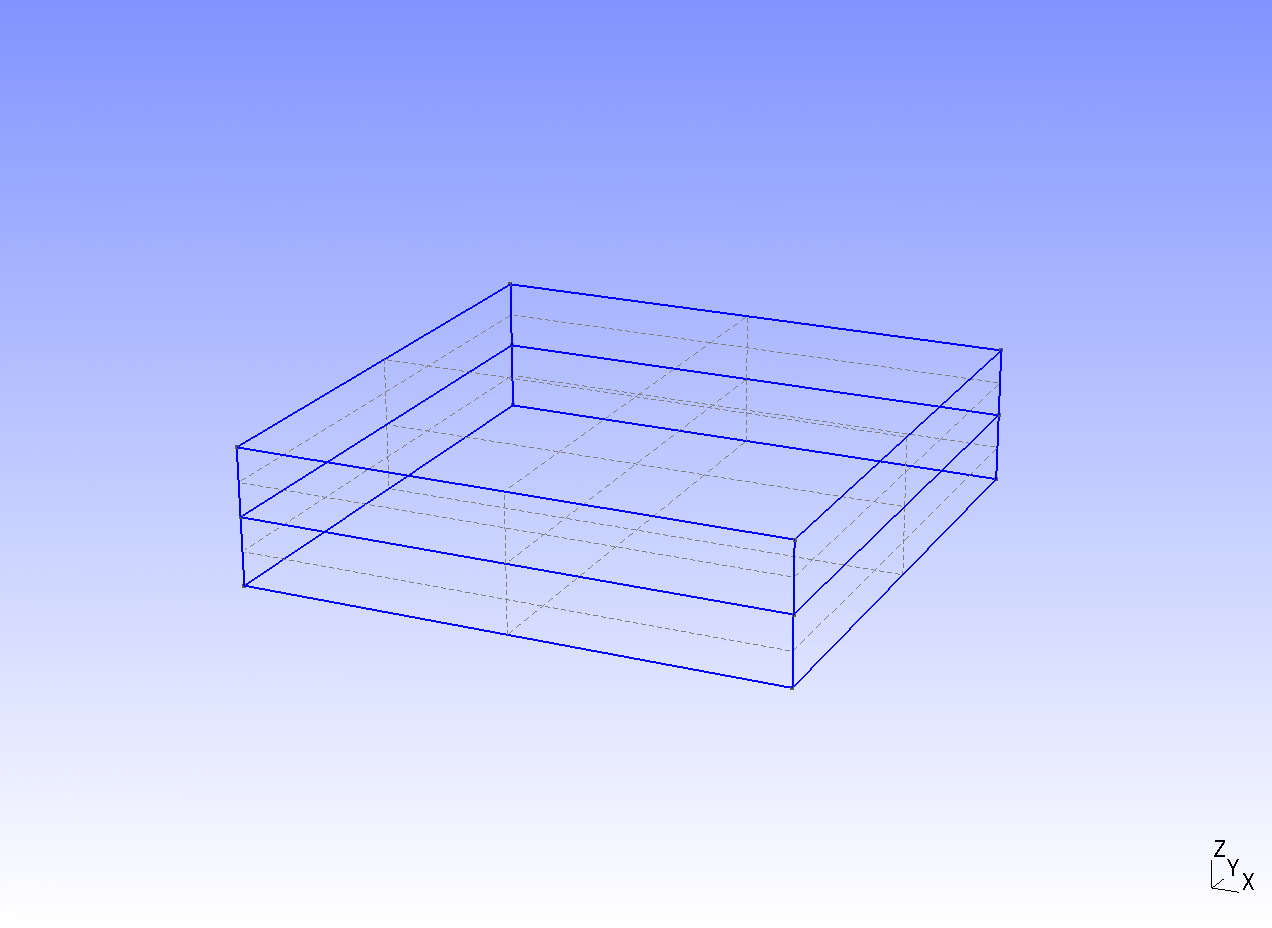
\includegraphics[width=3.5in]{figures/gmsh-example09m.png}}
\end{subfigure}
\begin{subfigure}[Gmesh view of a 200m 2D mesh on the domain surfaces.]
{\label{fig:gmsh3dmsh}
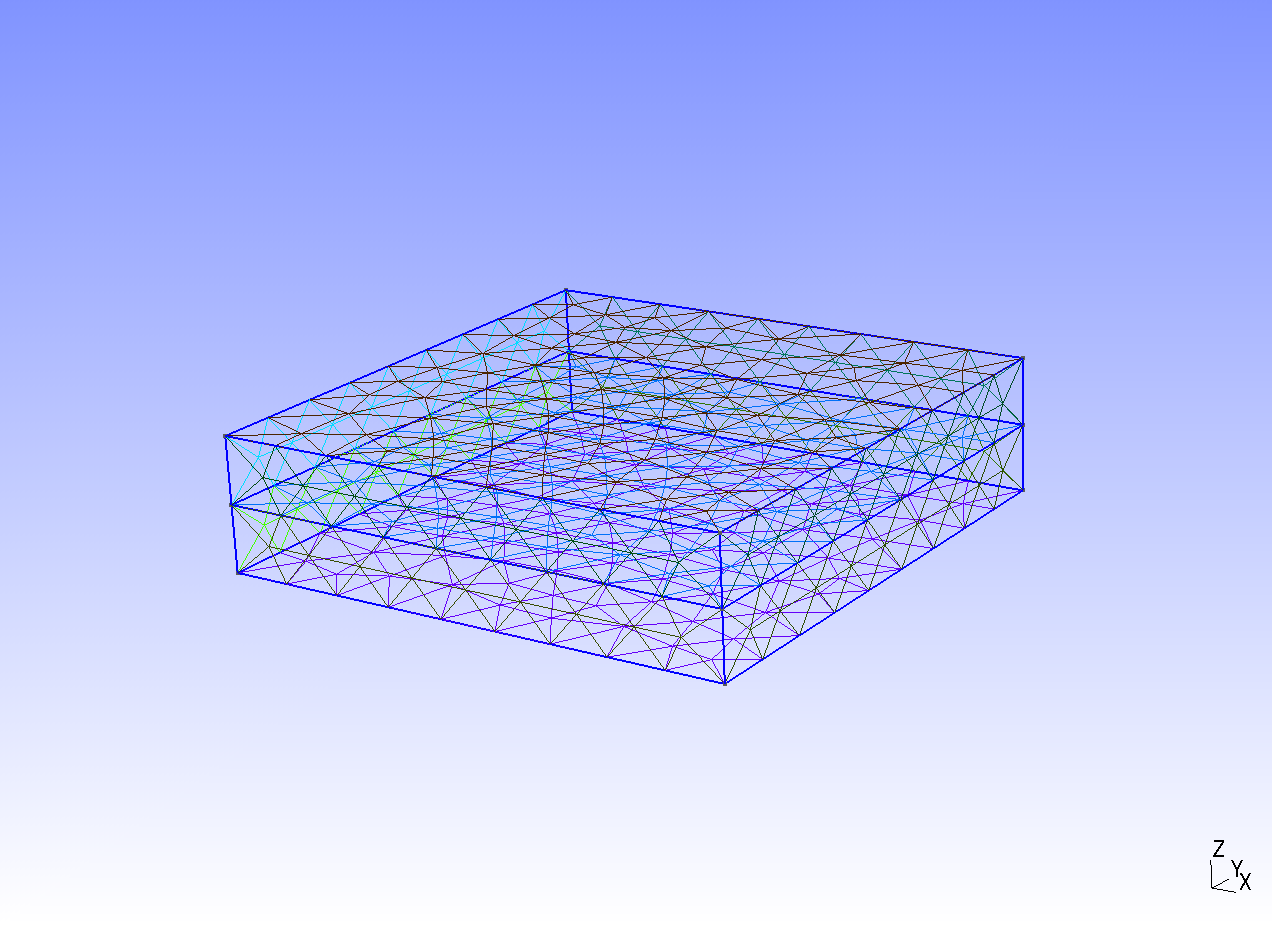
\includegraphics[width=3.5in]{figures/gmsh-example09msh2d.png}}
\end{subfigure}
\begin{subfigure}[Gmesh view of a 200m 3D mesh on the domain volumes.]
{\label{fig:gmsh3dmsh}
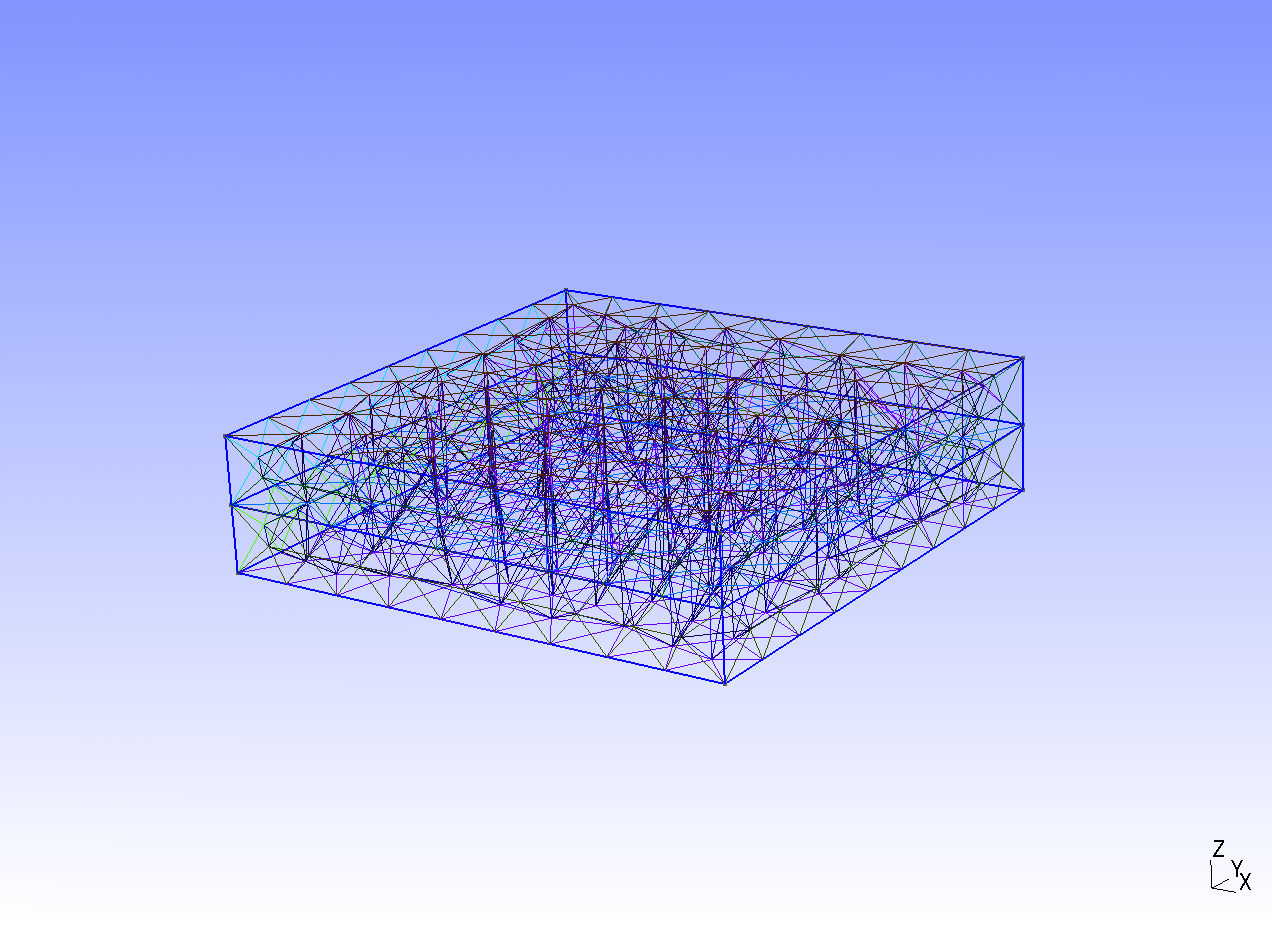
\includegraphics[width=3.5in]{figures/gmsh-example09msh3d.png}}
\end{subfigure}
\end{center}
\end{figure}
\clearpage

\section{Layer Cake Models}
Whilst this type of model seems simple enough to construct for two layers,
specifying multiple layers can become cumbersome. A function exists to generate
layer cake models called \verb!layer_cake!. A detailed description of its
arguments and returns is available in the API and the function can be imported
from the pycad.extras module.
\begin{python}
from esys.pycad.extras import layer_cake
intfaces=[10,30,50,55,80,100,200,250,400,500]

domaindes=Design(dim=3,element_size=element_size,order=2)
cmplx_domain=layer_cake(domaindes,xwidth,ywidth,intfaces)
cmplx_domain.setScriptFileName(os.path.join(save_path,"example09lc.geo"))
cmplx_domain.setMeshFileName(os.path.join(save_path,"example09lc.msh"))
dcmplx=MakeDomain(cmplx_domain)
dcmplx.write(os.path.join(save_path,"example09lc.fly"))
\end{python}

\begin{figure}[ht]
\begin{center}
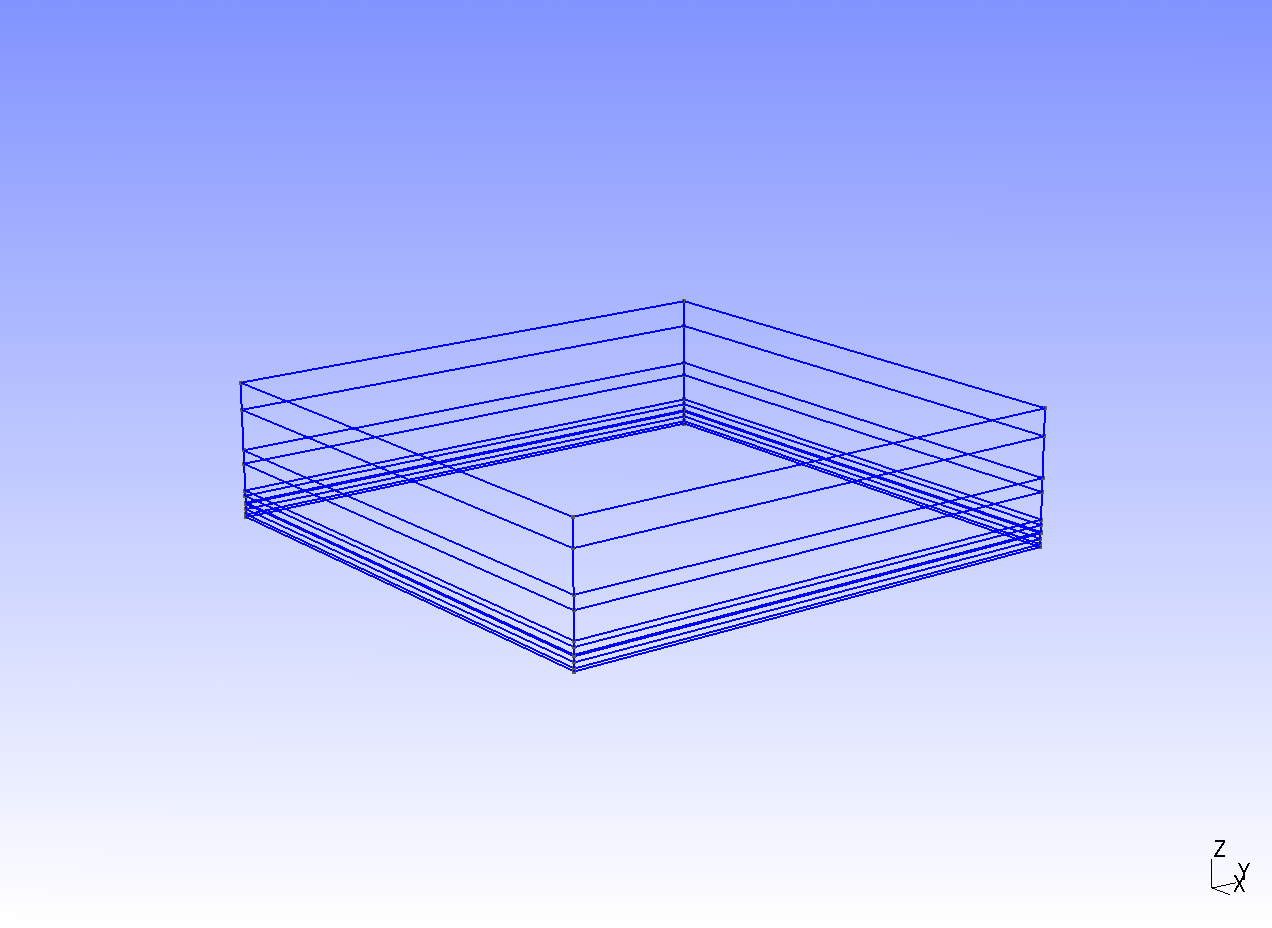
\includegraphics[width=5in]{figures/gmsh-example09lc.png}
\caption{Example geometry using layer cake function.}
\label{fig:gmsh3dlc}
\end{center}
\end{figure}
\clearpage
\section{Troubleshooting Pycad}
There are some techniques which can be useful when trying to troubleshoot
problems with pycad. As mentioned earlier it is important to ensure the correct
directionality of your primitives when constructing more complicated domains. If
it remains too difficult to establish the tangent of a line or curveloop, or
the normal of a surface, these values can be checked by importing the geometry
to gmesh and applying the appropriate visualisation options.

\section{3D Seismic Wave Propagation}
Adding an extra dimension to our wave equation solution script should be
relatively simple. Apart from the changes to the domain and therefore the
parameters of the model, there are only a few minor things which must be
modified to make the solution appropriate for 3d modelling.

\section{Applying a function to a domain tag}
\sslist{example09a.py}
To apply a function or data object to a domain requires a two step process. The
first step is to create a data object with an on/off mask based upon the tagged
value. This is quite simple and can be achieved by using a scalar data object
based upon the domain. In this case we are using the \verb!FunctionOnBoundary!
function space because the tagged value \verb!'stop'! is effectively a specific
subsurface of the boundary of the whole domain. 
\begin{python}
stop=Scalar(0.0,FunctionOnBoundary(domain))
stop.setTaggedValue("stop",1.0)
\end{python}
Now the data object \verb|stop| has the value 1.0 on the surface
\verb!'stop'! and zero everywhere else.
% 
 To apply our function to the boundary only on \verb|stop| we now
 mulitply it by \verb|stop|
\begin{python}
xb=FunctionOnBoundary(domain).getX()
yx=(cos(length(xb-xc)*3.1415/src_length)+1)*whereNegative(length(xb-xc)-src_length)
src_dir=numpy.array([0.,0.,1.0]) # defines direction of point source as down
mypde.setValue(y=source[0]*yx*src_dir*stop) #set the source as a function on the boundary
\end{python}

\section{Mayavi2 with 3D data.}
There are a variety of visualisation options available when using VTK data. The
types of visualisation are often data and interpretation specific and thus
consideration must be given to the type of output saved to file. Whether that is
scalar, vector or tensor data.

\begin{figure}[htp]
\centering
\begin{subfigure}[Example 9 at time step 201.]
 	{\label{fig:ex9b 201}
 	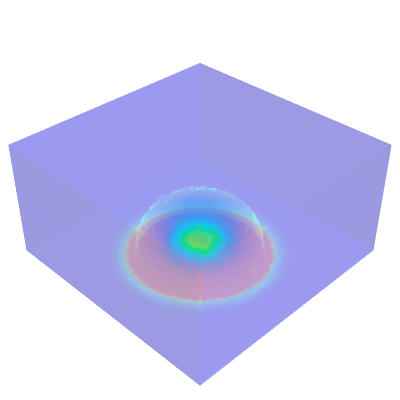
\includegraphics[width=0.45\textwidth]{figures/ex09b00201.png}}
 \end{subfigure}
 \begin{subfigure}[Example 9 at time step 341.]
 	{\label{fig:ex9b 201}
 	\includegraphics[width=0.45\textwidth]{figures/ex09b00341.png}}
 \end{subfigure}\\
 \begin{subfigure}[Example 9 at time step 440.]
 	{\label{fig:ex9b 201}
 	\includegraphics[width=0.45\textwidth]{figures/ex09b00440.png}}
 \end{subfigure}
\end{figure}

 
\chapter{Potential Fields - Newtonian Gravitation}
 
%%%%%%%%%%%%%%%%%%%%%%%%%%%%%%%%%%%%%%%%%%%%%%%%%%%%%%%%
%
% Copyright (c) 2003-2010 by University of Queensland
% Earth Systems Science Computational Center (ESSCC)
% http://www.uq.edu.au/esscc
%
% Primary Business: Queensland, Australia
% Licensed under the Open Software License version 3.0
% http://www.opensource.org/licenses/osl-3.0.php
%
%%%%%%%%%%%%%%%%%%%%%%%%%%%%%%%%%%%%%%%%%%%%%%%%%%%%%%%%

\section{Newtonian Potential}

In this chapter the gravitational potential field is developed for \esc.
Gravitational fields are present in many modelling scenarios, including
geophysical investigations, planetary motion and attraction and micro-particle
interactions. Gravitational fields also present an opportunity to demonstrate
the saving and visualisation of vector data for Mayavi, and the construction of
variable sized meshes.

The gravitational potential $U$ at a point $P$ due to a region with a mass
distribution of density $\rho(P)$, is given by Poisson's equation
\citep{Blakely1995}
\begin{equation} \label{eqn:poisson}
\nabla^2 U(P) = -4\pi\gamma\rho(P)
\end{equation}
where $\gamma$ is the gravitational constant.
Consider now the \esc general form, 
\autoref{eqn:poisson} requires only two coefficients,
$A$ and $Y$, thus the relevant terms of the general form are reduced to;
\begin{equation}
-\left(A_{jl} u_{,l} \right)_{,j} = Y
\end{equation}
One recognises that the LHS side is equivalent to 
\begin{equation} \label{eqn:ex10a}
-\nabla A \nabla u
\end{equation}
and when $A=\delta_{jl}$, \autoref{eqn:ex10a} is equivalent to
\begin{equation*}
-\nabla^2 u
\end{equation*}
Thus Poisson's \autoref{eqn:poisson} satisfies the general form when
\begin{equation}
A=\delta_{jl} \text{ and } Y= 4\pi\gamma\rho
\end{equation}
The boundary condition is the last parameter that requires consideration. The
potential $U$ is related to the mass of a sphere by
\begin{equation}
U(P)=-\gamma \frac{m}{r^2}
\end{equation} where $m$ is the mass of the sphere and $r$ is the distance from
the center of the mass to the observation point $P$. Plainly, the magnitude
of the potential is governed by an inverse-square distance law. Thus, in the
limit as $r$ increases;
\begin{equation}
\lim_{r\to\infty} U(P) = 0
\end{equation}
Provided that the domain being solved is large enough, and the source mass is
contained within a central region of the domain, the potential will decay to
zero. This is a dirichlet boundary condition where $U=0$.

This boundary condition can be satisfied when there is some mass suspended in a
free-space. For geophysical models where the mass of interest may be an anomaly
inside a host rock, the anomaly can be isolated by subtracting the density of the
host rock from the model. This creates a fictitious free space model that will
satisfy the analytic boundary conditions. The result is that
$Y=4\pi\gamma\Delta\rho$, where $\Delta\rho=\rho-\rho_0$ and $\rho_0$ is the
baseline or host density. This of course means that the true gravity response is
not being modelled, but the response due to an anomalous mass with a
density contrast $\Delta\rho$.

For this example we have set all of the boundaries to zero but only one boundary
point needs to be set for the problem to be solvable. The normal flux condition
is also zero by default. Note, that for a more realistic and complicated models
it may be necessary to give careful consideration to the boundary conditions of the model,
which can have an influence upon the solution.

Setting the boundary condition is relatively simple using the \verb!q! and
\verb!r! variables of the general form. First \verb!q! is defined as a masking
function on the boundary using
\begin{python}
q=whereZero(x[1]-my)+whereZero(x[1])+whereZero(x[0])+whereZero(x[0]-mx)
mypde.setValue(q=q,r=0)
\end{python}
This identifies the points on the boundary and \verb!r! is simply
ser to \verb!r=0.0!. This is a Dirichlet boundary condition.

\clearpage
\section{Gravity Pole}
\sslist{example10a.py}
A gravity pole is used in this example to demonstrate the vector characteristics
of gravity, and also to demonstrate how this information can be exported for
visualisation to Mayavi or an equivalent using the VTK data format.

The solution script for this section is very simple. First the domain is
constructed, then the parameters of the model are set, and finally the steady
state solution is found. There are quite a few values that can now be derived
from the solution and saved to file for visualisation.

The potential $U$ is related to the gravitational response $\vec{g}$ via
\begin{equation}
\vec{g} = \nabla U
\end{equation}
$\vec{g}$ is a vector and thus, has a a vertical component $g_{z}$ where
\begin{equation}
g_{z}=\vec{g}\cdot\hat{z}
\end{equation}
Finally, there is the magnitude of the vertical component $g$ of
$g_{z}$
\begin{equation}
g=|g_{z}|
\end{equation}
These values are derived from the \esc solution \verb!sol! to the potential $U$
using the following commands
\begin{python}
g_field=grad(sol) #The gravitational acceleration g.
g_fieldz=g_field*[0,1] #The vertical component of the g field.
gz=length(g_fieldz) #The magnitude of the vertical component.
\end{python}
This data can now be simply exported to a VTK file via
\begin{python}
# Save the output to file.
saveVTK(os.path.join(save_path,"ex10a.vtu"),\
        grav_pot=sol,g_field=g_field,g_fieldz=g_fieldz,gz=gz)
\end{python}

It is quite simple to visualise the data from the gravity solution in Mayavi2.
With Mayavi2 open go to File, Load data, Open file \ldots as in
\autoref{fig:mayavi2openfile} and select the saved data file. The data will
have then been loaded and is ready for visualisation. Notice that under the data
object in the Mayavi2 navigation tree the 4 values saved to the VTK file are
available (\autoref{fig:mayavi2data}). There are two vector values,
\verb|gfield| and \verb|gfieldz|. Note that to plot both of these on the same
chart requires that the data object be imported twice.

The point scalar data \verb|grav_pot| is the gravitational potential and it is
easily plotted using a surface module. To visualise the cell data a filter is
required that converts to point data. This is done by right clicking on the data
object in the explorer tree and selecting the cell to point filter as in
\autoref{fig:mayavi2cell2point}.

The settings can then be modified to suit personal taste. An example of the
potential and gravitational field vectors is illustrated in
\autoref{fig:ex10pot}.

\begin{figure}[ht]
\centering
\includegraphics[width=0.75\textwidth]{figures/mayavi2_openfile.png}
\caption{Open a file in Mayavi2}
\label{fig:mayavi2openfile}
\end{figure}

\begin{figure}[ht]
\centering
\includegraphics[width=0.75\textwidth]{figures/mayavi2_data.png}
\caption{The 4 types of data in the imported VTK file.}
\label{fig:mayavi2data}
\end{figure}

\begin{figure}[ht]
\centering
\includegraphics[width=0.75\textwidth]{figures/mayavi2_cell2point.png}
\caption{Converting cell data to point data.}
\label{fig:mayavi2cell2point}
\end{figure}

\begin{figure}[ht]
\centering
\includegraphics[width=0.75\textwidth]{figures/ex10apot.png}
\caption{Newtonian potential with $\vec{g}$ field directionality. The magnitude
of the field is reflected in the size of the vector arrows.}
\label{fig:ex10pot}
\end{figure}
\clearpage

\section{Gravity Well}
\sslist{example10b.py}
Let us now investigate the effect of gravity in three dimensions. Consider a
volume which contains a spherical mass anomaly and a gravitational potential
which decays to zero at the base of the model.

The script used to solve this model is very similar to that used for the gravity
pole in the previous section, but with an extra spatial dimension. As for all
the 3D problems examined in this cookbook, the extra dimension is easily
integrated into the \esc solution script.

The domain is redefined from a rectangle to a Brick;
\begin{python}
domain = Brick(l0=mx,l1=my,n0=ndx, n1=ndy,l2=mz,n2=ndz)
\end{python}
the source is relocated along $z$;
\begin{python}
x=x-[mx/2,my/2,mz/2]
\end{python}
and, the boundary conditions are updated.
\begin{python}
q=whereZero(x[2]-inf(x[2]))
\end{python}
No modifications to the PDE solution section are required. Thus the migration
from a 2D to a 3D problem is almost trivial.

\autoref{fig:ex10bpot} illustrates the strength of a PDE solution. Three
different visualisation types help define and illuminate properties of the data.
The cut surfaces of the potential are similar to a 2D section for a given x or y
and z. The iso-surfaces illuminate the 3D shape of the gravity field, as well as
its strength which is illustrated by the colour. Finally, the streamlines
highlight the directional flow of the gravity field in this example.

The boundary conditions were discussed previously, but not thoroughly
investigated. It was stated, that in the limit as the boundary becomes more
remote from the source, the potential will reduce to zero.
\autoref{fig:ex10bpot2} is the solution to the same gravity problem
but with a slightly larger domain. It is obvious in this case that
the previous domain size was too small to accurately represent the
solution. The profiles in \autoref{fig:ex10p} further demonstrates the affect
the domain size has upon the solution. As the domain size increases, the
profiles begin to converge. This convergence is a good indicator of an
appropriately dimensioned model for the problem, and and sampling location. 

\begin{figure}[htp]
\centering
\includegraphics[width=0.75\textwidth]{figures/ex10bpot.png}
\caption{Gravity well with iso surfaces and streamlines of the vector
gravitational potential \textemdash small model.}
\label{fig:ex10bpot}
\end{figure}

\begin{figure}[htp]
\centering
\includegraphics[width=0.75\textwidth]{figures/ex10bpot2.png}
\caption{Gravity well with iso surfaces and streamlines of the vector
gravitational potential \textemdash large model.}
\label{fig:ex10bpot2}
\end{figure}

\begin{figure}[htp]
\centering
\includegraphics[width=0.85\textwidth]{figures/ex10p_boundeff.pdf}
\caption{Profile of the graviational provile along x where $y=0,z=250$ for
various sized domains.}
\label{fig:ex10p}
\end{figure}
\clearpage

\section{Gravity Surface over a fault model.}
\sslist{example10c.py,example10m.py}
This model demonstrates the gravity result for a more complicated domain which
contains a fault. Additional information will be added when geophysical boundary
conditions for a gravity scenario have been established.

\begin{figure}[htp]
\centering
\subfigure[The geometry of the fault model in example10c.py.]
	{\label{fig:ex10cgeo}
	 \includegraphics[width=0.8\textwidth]{figures/ex10potfaultgeo.png}} \\
\subfigure[The fault of interest from the fault model in
	example10c.py.] 
	{\label{fig:ex10cmsh}
	 \includegraphics[width=0.8\textwidth]{figures/ex10potfaultmsh.png}}
\end{figure}

\begin{figure}[htp]
\centering
	\includegraphics[width=0.8\textwidth]{figures/ex10cpot.png}
	\caption{Gravitational potential of the fault model with primary layers and
	faults identified as isosurfaces.}
	\label{fig:ex10cpot}
\end{figure}
\clearpage

\section{Variable mesh-element sizes}
\sslist{example10m.py}
We saw in a previous section that the domain needed to be sufficiently
large for the boundary conditions to be satisfied. This can be troublesome when
trying to solve problems that require a dense mesh, either for solution
resolution of stability reasons. The computational cost of solving a large
number of elements can be prohibitive.S

With the help of Gmsh, it is possible to create a mesh for \esc, which has a
variable element size. Such an approach can significantly reduce the number of
elements that need to be solved, and a large domain can be created that has
sufficient resolution close to the source and extends to distances large enough
that the infinity clause is satisfied.

To create a variable size mesh, multiple meshing domains are required. The
domains must share points, boundaries and surfaces so that they are joined; and
no sub-domains are allowed to overlap. Whilst this initially seems complicated,
it is quite simple to implement. 

This example creates a mesh which contains a high resolution sub-domain at its
center. We begin by defining two curve loops which describe the large or
big sub-domain and the smaller sub-domain which is to contain the high
resolution portion of the mesh. 
\begin{python}
################################################BIG DOMAIN
#ESTABLISHING PARAMETERS
width=10000.    #width of model
depth=10000.    #depth of model
bele_size=500.  #big element size
#DOMAIN CONSTRUCTION
p0=Point(0.0,    0.0)
p1=Point(width, 0.0)
p2=Point(width, depth)
p3=Point(0.0,   depth)
# Join corners in anti-clockwise manner.
l01=Line(p0, p1)
l12=Line(p1, p2)
l23=Line(p2, p3)
l30=Line(p3, p0)

cbig=CurveLoop(l01,l12,l23,l30)

################################################SMALL DOMAIN
#ESTABLISHING PARAMETERS
xwidth=2000.0   #x width of model
zdepth=2000.0   #y width of model
sele_size=10.   #small element size
#TRANSFORM
xshift=width/2-xwidth/2
zshift=depth/2-zdepth/2
#DOMAIN CONSTRUCTION
p4=Point(xshift, zshift)
p5=Point(xwidth+xshift, zshift)
p6=Point(xwidth+xshift, zdepth+zshift)
p7=Point(xshift,    zdepth+zshift)
# Join corners in anti-clockwise manner.
l45=Line(p4, p5)
l56=Line(p5, p6)
l67=Line(p6, p7)
l74=Line(p7, p4)

csmall=CurveLoop(l45,l56,l67,l74)
\end{python}
The small sub-domain curve can then be used to create a surface.
\begin{python}
ssmall=PlaneSurface(csmall)
\end{python}
However, so that the two domains do not overlap, when the big sub-domain
curveloop is used to create a surface it must contain a hole. The hole is
defined by the small sub-domain curveloop.
\begin{python}
sbig=PlaneSurface(cbig,holes=[csmall])
\end{python}
The two sub-domains now have a common geometry and no over-laping features as
per \autoref{fig:ex10mgeo}. Notice, that both domains have a normal in the
same direction.

The next step, is exporting each sub-domain individually, with an appropriate
element size. This is carried out using the \pycad Design command.
\begin{python}
# Design the geometry for the big mesh.
d1=Design(dim=2, element_size=bele_size, order=1)
d1.addItems(sbig)
d1.addItems(PropertySet(l01,l12,l23,l30))
d1.setScriptFileName(os.path.join(save_path,"example10m_big.geo"))
MakeDomain(d1)

# Design the geometry for the small mesh.
d2=Design(dim=2, element_size=sele_size, order=1)
d2.addItems(ssmall)
d2.setScriptFileName(os.path.join(save_path,"example10m_small.geo"))
MakeDomain(d2)
\end{python}
Finally, a system call to Gmsh is required to merge and then appropriately
mesh the two sub-domains together.
\begin{python}
# Join the two meshes using Gmsh and then apply a 2D meshing algorithm.
# The small mesh must come before the big mesh in the merging call!!@!!@!
sp.call("gmsh -2 "+
        os.path.join(save_path,"example10m_small.geo")+" "+
        os.path.join(save_path,"example10m_big.geo")+" -o "+
        os.path.join(save_path,"example10m.msh"),shell=True)
\end{python}
The ``-2'' option is responsible for the 2D meshing, and the ``-o'' option
provides the output path. The resulting mesh is depicted in
\autoref{fig:ex10mmsh}

To use the Gmsh ``*.msh'' file in the solution script, the mesh reading function
``ReadGmsh'' is required. It can be imported via;
\begin{python}
from esys.finley import ReadGmsh
\end{python}
To read in the file the function is called 
\begin{python}
domain=ReadGmsh(os.path.join(mesh_path,'example10m.msh'),2) # create the domain
\end{python}
where the integer argument is the number of domain dimensions.
% 
 \begin{figure}[ht]
\centering
\includegraphics[width=0.8\textwidth]{figures/ex10m_geo.png}
\caption{Geometry of two surfaces for a single domain.}
\label{fig:ex10mgeo}
\end{figure}

\begin{figure}[ht]
\centering
\includegraphics[width=0.8\textwidth]{figures/ex10m_msh.png}
\caption{Mesh of merged surfaces, showing variable element size. Elements
range from 10m in the centroid to 500m at the boundary.}
\label{fig:ex10mmsh}
\end{figure}
\clearpage

\section{Unbounded problems}
With a variable element-size, it is now possible to solve the potential problem
over a very large mesh. To test the accuracy of the solution, we will compare
the \esc result with the analytic solution for the vertical gravitational
acceleration $g_z$ of an infinite horizontal cylinder.

For a horizontal cylinder with a circular cross-section with infinite strike,
the analytic solution is give by
\begin{equation}
g_z = 2\gamma\pi R^2 \Delta\rho \frac{z}{(x^2+z^2)} 
\end{equation}
where $\gamma$ is the gravitational constant (as defined previously), $R$ is the
radius of the cylinder, $\Delta\rho$ is the density contrast and $x$ and $z$ are
geometric factors, relating the observation point to the center of the source
via the horizontal and vertical displacements respectively.

The accuracy of the solution was tested using a square domain. For each test the
dimensions of the domain were modified, being set to 5, 10, 20 and 40 Km. The
results are compared with the analytic solution and are depicted in
\autoref{fig:ex10q boundeff} and \autoref{fig:ex10q boundeff zoom}. Clearly, 
as the domain size increases, the results are valid at greater
distances from the source. The same is true at the anomaly peak, where the
variation around the source diminishes with an increasing domain size.

\begin{figure}[ht]
\centering
\includegraphics[width=0.8\textwidth]{figures/ex10q_boundeff.pdf}
\caption{Solution profile 1000.0 meters from the source as the domain size
increases.}
\label{fig:ex10q boundeff}
\end{figure}

\begin{figure}[ht]
\centering
\includegraphics[width=0.8\textwidth]{figures/ex10q_boundeff_zoom.pdf}
\caption{Magnification of \autoref{fig:ex10q boundeff}.}
\label{fig:ex10q boundeff zoom}
\end{figure}
\clearpage

\subsection{Inversion using scipy}
%  
\chapter{Potential Fields - Electrical Resistivity}
 
%%%%%%%%%%%%%%%%%%%%%%%%%%%%%%%%%%%%%%%%%%%%%%%%%%%%%%%%
%
% Copyright (c) 2003-2012 by University of Queensland
% Earth Systems Science Computational Center (ESSCC)
% http://www.uq.edu.au/esscc
%
% Primary Business: Queensland, Australia
% Licensed under the Open Software License version 3.0
% http://www.opensource.org/licenses/osl-3.0.php
%
%%%%%%%%%%%%%%%%%%%%%%%%%%%%%%%%%%%%%%%%%%%%%%%%%%%%%%%%

In this chapter we will investigate the effects of a current flow and
resistivity in a medium. This type of problem is related to the DC resistivity method of
geophysical prospecting. Currents are injected into the ground at the surface
and measurements of the potential are taken at various potential-dipole
locations along or adjacent to the survey line. From these measurements of the
potential it is possible to infer an approximate apparent resistivity model of
the subsurface.

The following theory comes from a tutorial by \citet{Loke2004}.
We know from Ohm's law that the current flow in the ground is given in vector
form by
\begin{equation}
\vec{J}=\sigma\vec{E}
\end{equation}
where $\vec{J}$ is current density, $\vec{E}$ is the electric field intensity
and $\sigma$ is the conductivity. We can relate the potential to the electric
field intensity by 
\begin{equation}
E=-\nabla\Phi
\end{equation}
where $\Phi$ is the potential. We now note that the current density is related
to the potential via
\begin{equation}
\vec{J}=-\sigma\nabla\Phi
\end{equation}
Geophysical surveys predominantly use current sources which individually act as
point poles. Considering our model will contain volumes, we can normalise the
input current and approximate the current density in a volume $\Delta V$ by
\begin{equation}
\nabla \vec{J} =
\left(\frac{I}{\Delta V} \right) \delta(x-x_{s})
								 \delta(y-y_{s})
								 \delta(z-z_{s})
\end{equation}

\begin{equation}
-\nabla \cdot \left[ \sigma(x,y,z) \nabla \phi (x,y,z) \right] =
\left(\frac{I}{\Delta V} \right) \delta(x-x_{s})
								 \delta(y-y_{s})
								 \delta(z-z_{s})			 
\end{equation}

This form is quite simple to solve in \esc.

\section{3D Current-Dipole Potential}
\sslist{example11m.py; example11c.py}

\begin{figure}[ht]
\centering
\includegraphics[width=0.95\textwidth]{figures/ex11cstreamline.png}
\caption{Current Density Model for layered medium.}
\label{fig:ex11cstream}
\end{figure}

\section{Frequency Dependent Resistivity - Induced Polarisation}
With a more complicated resistivity model it is possible to calculate the
chargeability or IP effect in the model. A recent development has been the
Fractal model for complex resistivity \citep{Farias2010,Honig2007}.


The model is calculated over many frequencyies and transformed to the time
domain using a discrete fourier transform.




\bibliography{cookbook}
\bibliographystyle{plainnat}

\appendix
%
%%%%%%%%%%%%%%%%%%%%%%%%%%%%%%%%%%%%%%%%%%%%%%%%%%%%%%%%%%%%%%%%%%%%%%%%%%%%%%
% Copyright (c) 2003-2012 by University of Queensland
% http://www.uq.edu.au
%
% Primary Business: Queensland, Australia
% Licensed under the Open Software License version 3.0
% http://www.opensource.org/licenses/osl-3.0.php
%
% Development until 2012 by Earth Systems Science Computational Center (ESSCC)
% Development since 2012 by School of Earth Sciences
%
%%%%%%%%%%%%%%%%%%%%%%%%%%%%%%%%%%%%%%%%%%%%%%%%%%%%%%%%%%%%%%%%%%%%%%%%%%%%%%

\chapter{The Einstein Summation Convention}

The Einstein Summation Convention (ESC) is a notational convention that is prefered by the \esc developers. It is a condensed and practical way to deal with multi-dimensional and convoluted PDEs. By suppressing the need to write out the many terms of each problem it is possible to increase efficiency and reduce the number of errors created through poor working. According to the convention, when an index variable appears twice in a single term, it implies that we are summing over all of its possible values.
So we have;
\begin{equation}
a_{1}\frac{\partial^2 f}{\partial x_{1}^2} + a_{2}\frac{\partial^2 f}{\partial x_{2}^2} = a_{i}\frac{\partial^2 f}{\partial x_{i}^2}
\end{equation}

For a scalar function $f(x_{1},x_{2},..x_{i})$ and a vector $\mathbf{u}(u_{1},u_{2},..u_{i})$ with $u_{i}(x_{1},x_{2},..x_{i})$, we have the following notation:
\begin{equation}
\mathbf{u}=\sum_{i}u_{i}e^i = u_{i}e^i
\end{equation}
\begin{equation}
\mathbf{grad}(f) = \mathbf{\nabla}(f) = \sum_{i}\frac{\partial f}{\partial x_{i}}e^i = (\partial_{i} f)e^i = f_{,i}e^i
\end{equation}
\begin{equation}
div(\mathbf{u}) = \mathbf{\nabla}.\mathbf{u} = \sum_{i}\frac{\partial u_{i}}{\partial x_{i}} = \partial_{i} u_{i} = u_{i,i}
\end{equation}
\begin{equation}
div(\mathbf{grad}(f)) = \nabla^2 f = \Delta f = \sum_{i}\frac{\partial^2 f}{\partial x_{i}^2} = f_{,ii}
\end{equation}

\printindex
\end{document}
